
\begin{appendices} 

\chapter{Millepede}
\label{annexe:Millepede}

   La m\'ethode d'alignement \texttt{Millepede} \cite{Blobel:2002ax} \cite{Blobel20065} fait partie des m\'ethodes dites globales. Bien que cette m\'ethode soit obtenue d'une façon diff\'erente de celle expos\'ee plus haut, le r\'esultat est \'equivalent.
   
   \medskip
   
   Le point cl\'e de la m\'ethode est l'ajustement simultan\'e des toutes les traces et de tous les param\`etres d'alignement. Les param\`etres des traces sont appel\'es param\`etres locaux alors que les param\`etres de l'alignement sont appel\'es param\`etres globaux.
   
   Les r\'esidus $r_{ij}$ peuvent \^etre \'ecrits en fonction de la mesure de l'impact $m_{ij}$ et du mod\`ele d'extrapolation de la trace $j$ : $f(\mathbf{q_j^{local}},\mathbf{p^{global}})$  :
   
   \begin{equation}
   r_{ij} = m_{ij} - f(\mathbf{q_j^{local}},\mathbf{p^{global}})
   \end{equation}
   
   Pour simplifier l'\'ecriture nous allons utiliser les nouvelles notations $\mathbf{q_j^{local}} = \mathbf{q_j}$ correspondant aux param\`etres de la trace $j$ et $\mathbf{p^{global}} = \mathbf{p}$ correspondant au vecteur des param\`etres d'alignement.
   
   \medskip
   
   En diff\'erentiant les r\'esidus, on obtient :
   
   \begin{equation}
   \Delta r_{ij} = -\left( \mathbf{\delta_{local}^T} \mathbf{\Delta q_j} + \mathbf{d_{global}^T} \mathbf{\Delta p} \right)
   \end{equation}
   
   Avec $\Delta r_{ij}$ la variation des r\'esidus correspondant \`a l'impact $i$ par rapport aux variations des param\`etres $q_j$ : $\mathbf{\delta_{local}^T}$ de la trace $j$ ; et aux variations $\mathbf{d_{global}^T}$ des param\`etres de l'alignement $p$ des capteurs/modules. On a alors :
   
   \begin{equation}
    \mathbf{\delta_{ij}^T} \equiv \mathbf{\delta_i^T} = \cfrac{\partial f(\mathbf{q_j},\mathbf{p})}{\partial \mathbf{q_j} }
   \end{equation}

   et, 
   
   \begin{equation}
     \mathbf{d_{ij}^T} \equiv \mathbf{d_i^T} = \cfrac{\partial f(\mathbf{q_j},\mathbf{p})}{\partial \mathbf{p} }
   \end{equation}
   
   et avec : $\mathbf{\Delta q_j} = \mathbf{q_j} - \mathbf{q_j(0)}$ et $ \mathbf{\Delta p} = \mathbf{p} - \mathbf{p(0)} $.
   
   \medskip
   
   Les r\'esidus peuvent alors \^etre exprim\'es en tenant compte de cette correction. On a alors la relation suivante :
   
   \begin{equation}
   r_{ij} = m_{ij} - \Delta r_{ij} = m_{ij} + \left( \mathbf{\delta_i^T} \mathbf{\Delta q_j} + \mathbf{d_i^T} \mathbf{\Delta p} \right)
   \end{equation}
   
   Une fois ce mod\`ele \'etabli, on peut proc\'eder \`a la minimisation du $\chi^2$ suivant :
   
   \begin{equation}
    \chi^2(\mathbf{Q_j}, \mathbf{P}) = \sum_{ij} \cfrac{ \left( m_{ij} + \mathbf{\delta_i^T} \mathbf{\Delta q_j} + \mathbf{d_i^T} \mathbf{\Delta p} \right)^2}{\sigma_{ij}^2}
   \end{equation}

   O\`u l'on somme sur toutes les traces $j$ et toutes les mesures $i$.
   Pour plus de clart\'e nous allons renommer certaines variables. On prendra par la suite : $\mathbf{\Delta p} = \mathbf{P}$ et $\mathbf{\Delta q_j} = \mathbf{Q_j}$. \`A partir d'ici, $P$ et $Q_j$ repr\'esentent les corrections aux param\`etres d'alignement et aux param\`etres des traces.
   
   \medskip
   
   L'objectif est de minimiser ce $\chi^2$ global en ajustant simultan\'ement les param\`etres de l'alignement et les param\`etres des traces. On se sert alors de la relation suivante :
   
   \begin{equation}
    \cfrac{\partial \left( \mathbf{Y^T Z} \right) }{\partial \mathbf{X}} = \mathbf{Z^T} \cfrac{\partial \mathbf{Y} }{\partial \mathbf{X}} + \mathbf{Y^T} \cfrac{\partial \mathbf{Z} }{\partial \mathbf{X}}
   \end{equation}

   O\`u $\mathbf{X}$, $\mathbf{Y}$ et $\mathbf{Z}$ sont des vecteurs.
   
   \medskip
   
   Ce qui nous donne pour toutes les traces et les mesures $i$ :
  
   \begin{equation}
   \begin{cases}
     \cfrac{\partial \chi^2 }{\partial \mathbf{P} } = 2 \sum_{ij} \omega_{ij} \left( \mathbf{P^T} \mathbf{d_i} \mathbf{d_i^T} - (m_{ij} - \mathbf{\delta_i^T} \mathbf{Q_j} ) \mathbf{d_i^T} \right) = \mathbf{0} \\
     \text{Et si les param\`etres des diff\'erentes traces sont ind\'ependants,} \\
     \text{pour chaque trace $j$ on a :} \\
     \cfrac{\partial \chi^2 }{\partial \mathbf{Q_j} } = 2 \sum_{ij} \omega_{ij} \left( \mathbf{Q_j^T} \mathbf{\delta_i} \mathbf{\delta_i^T} - ( m_{ij} - \mathbf{d_i^T} \mathbf{P} ) \mathbf{\delta_i^T} \right) = \mathbf{0}
   \end{cases}
   \label{eq:syst_millepde}
   \end{equation}

   Ces deux syst\`emes d'\'equations peuvent \^etre reformul\'es de la fa\c{c}on suivante :
   
   \begin{equation}
   \begin{cases}
   \sum_{ij} \omega_{ij} \left( \mathbf{d_i} \, \mathbf{d_i^T} \, \mathbf{P} + \mathbf{d_i} \, \mathbf{\delta_i^T} \, \mathbf{Q_j} \right) = \sum_{ij} \omega_{ij} \, \mathbf{d_i} \, m_{ij} \\
   \sum_j \omega_{ij} \left( \mathbf{\delta_i} \, \mathbf{\delta_i^T} \, \mathbf{Q_j} + \mathbf{\delta_i} \, \mathbf{d_i^T} \, \mathbf{P} \right) = \sum_j \omega_{ij} \, \mathbf{\delta_i} \, m_{ij}
   \end{cases}
   \end{equation}
   
   Pour simplifier l'\'ecriture on va renommer les matrices et vecteurs pr\'esents dans ces deux syst\`emes.
   
   \begin{equation}
    \begin{cases}
     C_j = \sum_i \omega_{ij} \, \mathbf{d_i} \, \mathbf{d_i^T} \\
     G_i = \sum_i \omega_{ij} \, \mathbf{d_i} \, \mathbf{\delta_i^T} \\
     b_i = \sum_i \omega_{ij} \, \mathbf{d_i} \, m_{ij} \\
     \Gamma_i = \sum_i \omega_{ij} \, \mathbf{\delta_i} \, \mathbf{\delta_i^T} \\
     \beta_i = \sum_i \omega{ij} \, \mathbf{\delta_i} \, m_{ij}
    \end{cases}
   \end{equation}

   S'il y a $N_c$ capteurs param\'etris\'es par $6$ degr\'es de libert\'es et $n$ traces dot\'ees de $m=5$ param\`etres, cela revient \`a r\'esoudre un syst\`eme de $N = 6 \, N_c + n \times m$ \'equations. Le temps de calcul pour un tel probl\`eme est proportionnel \`a $N^3$ et la m\'emoire consomm\'ee \`a $N^2$. Par exemple pour $n=10^5$ traces et $N_c = 10^3$ capteurs. Il faut r\'esoudre un syst\`eme de 506000 \'equations ! Le temps de calcul devient alors tr\`es \'elev\'e.
   
   \medskip
   
   Nous allons voir que gr\^ace aux propri\'et\'es de ce syst\`eme d'\'equations, on peut se ramener \`a l'inversion d'une matrice d\'ependant uniquement des param\`etres d'alignement. La taille de la matrice \`a inverser sera alors de $6N_c \times 6N_c$. Pour cela on va r\'esoudre le probl\`eme en partitionnant la matrice \'equivalente au syst\`eme d'\'equations \ref{eq:syst_millepde}. On exprime d'abord cette matrice \'equivalente :
   
   \begin{equation}
     \left(\begin{array}{c|cccccccccc}
     \sum\limits_{j} C_j & G_1 & \cdots & \cdots & G_l & \cdots & \cdots & G_k & \cdots & \cdots & G_n \\ \\ \hline \\
     G_1^T        & \Gamma_1 & 0 & \cdots & \cdots & \cdots & \cdots & \cdots & \cdots & \cdots & 0 \\
     \vdots & \vdots & \ddots & \vdots & \vdots & \vdots & \vdots & \vdots & \vdots & \vdots & \vdots \\
     \vdots & \vdots & \vdots & \ddots & \vdots & \vdots & \vdots & \vdots & \vdots & \vdots & \vdots \\
     G_l^T        & 0 & \cdots & 0 & \Gamma_l & 0 & \cdots & \cdots & \cdots & \cdots & 0 \\
     \vdots & \vdots & \vdots & \vdots & \vdots & \ddots & \vdots & \vdots & \vdots & \vdots & \vdots \\
     \vdots & \vdots & \vdots & \vdots & \vdots & \vdots & \ddots & \vdots & \vdots & \vdots & \vdots \\
     G_k^T        & 0 & \cdots & 0 & \cdots & \cdots & 0 & \Gamma_k & 0 & \cdots & 0 \\
     \vdots & \vdots & \vdots & \vdots & \vdots & \vdots & \vdots & \vdots & \ddots & \vdots & \vdots \\
     \vdots & \vdots & \vdots & \vdots & \vdots & \vdots & \vdots & \vdots & \vdots & \ddots & \vdots \\
     G_1^T        & 0 & \cdots & \cdots & \cdots & \cdots & \cdots & \cdots & \cdots & 0 & \Gamma_n
     \end{array}\right) \left(\begin{array}{c}
     \mathbf{P} \\ \\ \hline \\
     \mathbf{Q_1} \\
     \vdots \\
     \vdots \\
     \mathbf{Q_l} \\
     \vdots \\
     \vdots \\
     \mathbf{Q_k} \\
     \vdots \\
     \vdots \\
     \mathbf{Q_n}
     \end{array}\right) = \left(\begin{array}{c}
      \sum\limits_{j} b_j \\ \\ \hline \\
     \beta_1 \\
     \vdots \\
     \vdots \\
     \beta_l \\
     \vdots \\
     \vdots \\
     \beta_k \\
     \vdots \\
     \vdots \\
     \beta_n
     \end{array}\right)
     \label{eq:big_matrix}
   \end{equation}

   Identifions les termes. $\mathbf{P}$ est le vecteur des corrections pour les param\`etres d'alignement, $\mathbf{Q_j}$ est le vecteur des corrections pour les param\`etres de la trace $j$, $C_j$ est l'inverse de la matrice de covariance de la trace $j$ par rapport aux param\`etres d'alignement et $\Gamma_j$ est l'inverse de la matrice de covariance de la trace $j$ par rapport aux param\`etres de la trace. $G_j$ contient les covariances entre les param\`etres de la trace $j$ et les param\`etres d'alignement pour la trace $j$. Enfin, $b_i$ contient les d\'eriv\'ees selon les param\`etres d'alignement et $\beta_j$ contient les d\'eriv\'ees selon les param\`etres des traces.
   
   \medskip
   
   Comme nous sommes int\'eress\'es uniquement par les param\`etres de l'alignement, on peut remarquer la structure particuli\`ere de la relation \ref{eq:big_matrix}. On peut l'\'ecrire sous la forme compacte suivante :
   
   \begin{equation}
    \left(\begin{array}{c|c}
      M_{11} & M_{21}^T \\ \hline
      M_{21} & M_{22} \\
     \end{array}\right) \left(\begin{array}{c}
      \mathbf{P} \\ \hline
      \mathbf{Q} \\
     \end{array}\right) = \left(\begin{array}{c}
      \mathbf{b} \\ \hline
      \mathbf{\beta} \\
     \end{array}\right)
     \label{eq_big_matrix_compact}
   \end{equation}

   La solution \`a ce syst\`eme peut \^etre r\'e-\'ecrite en utilisant le \textit{compl\'ement de Schur} $S$ :
   
   \begin{equation}
     \left(\begin{array}{c}
      \mathbf{P} \\ \hline
      \mathbf{Q} \\
     \end{array}\right) = - \left(\begin{array}{c|c}
      S^{-1} & -S^{-1} \, M_{21}^T \, M_{22} \\ \hline
      -M_{22}^{-1} \, M_{21} \, S^{-1} & M_{22}^{-1} - M_{22}^{-1} \, M_{21} \, M_{21}^T \, S^{-1} \, M_{22}^{-1} \\
     \end{array}\right) \left(\begin{array}{c}
      \mathbf{b} \\ \hline
      \mathbf{\beta} \\
     \end{array}\right)
   \end{equation}
   
   \medskip
   
   Avec le compl\'ement de \textit{Schur} donn\'e par ,
   
   \begin{equation}
   S= M_{11} - M_{21}^{T} M_{22}^{-1} M_{21}
   \end{equation}
   
   \medskip
   
   Ainsi la solution pour le vecteur des corrections d'alignement $\mathbf{P}$ est la suivante :
   
   \begin{equation}
    \mathbf{P} = -S^{-1} \left( \mathbf{b} - M_{21}^T \, M_{22} \, \mathbf{\beta} \right)
   \end{equation}

%    On notera que la matrice $M_{22} = $ est bloc-diagonale puisque les les param\`etres des diff\'erentes traces ne sont pas corr\'el\'ees.
   On peut r\'e\'ecrire la relation pr\'ec\'edente en remplaçant les matrices $M$ et $S$ par leurs expressions. On a alors :
   
   \begin{equation}
    \mathbf{P} = \left[ \sum_j \left( C_j- G_j \, \Gamma_j^{-1} \, G_j^T \right) \right]^{-1} \, \sum_j \left( \mathbf{b_j} - G_j(\Gamma_j^{-1} \, \beta_j) \right)
   \end{equation}
   
   Ce qui donne sous une forme plus compact\'ee :
   
   \begin{equation}
    \mathbf{P} = A^{-1} \, \mathbf{b'}
   \end{equation}

   Avec : 
   
   \begin{equation}
    A = \sum_j \left( C_j- G_j \, \Gamma_j^{-1} \, G_j^T \right)
   \end{equation}
   
   et :
   
   \begin{equation}
    \mathbf{b'} = \sum_j \left( \mathbf{b_j} - G_j(\Gamma_j^{-1} \, \beta_j) \right) 
    \label{eq:b'}
   \end{equation}

   Les matrices $\Gamma_j$ contenues dans $A$ sont de petites tailles et sont donc tr\`es facilement inversables. La matrice $A$ \`a inverser a cette fois-ci une taille de $6N_c \times 6N_c$, lorsqu'il y a 6 degr\'es de libert\'e par capteur/module. La taille de cette matrice est alors fortement r\'eduite, et une inversion (beaucoup plus rapide) que celle du syst\`eme complet \ref{eq:syst_millepde} est alors possible. M\^eme si la m\'ethode est conçue pour aligner tous les capteurs en une seule it\'eration, la variation des r\'esidus en fonction des param\`etres des traces et des param\`etres d'alignement n'est pas toujours lin\'eaire. Cette non lin\'earit\'e implique de faire plusieurs it\'erations de la m\'ethode avant d'obtenir une convergence de l'alignement.
   
   \medskip
   
   Si l'on consid\`ere les param\`etres d'alignement constants dans la relation \ref{eq:big_matrix}, on peut remarquer que comme les corr\'elations des param\`etres entre deux traces sont nulles (Une trace ne d\'epend pas d'une autre) $M_{22}$ est bloc-diagonale. On peut alors r\'e-\'ecrire le syst\`eme pour chaque trace $j$ par :
   
   \begin{equation}
    \mathbf{Q_j} = \Gamma_j^{-1} \, \beta_j
    \label{eq:traces_locales_mille}
   \end{equation}

   Il s'agit l\`a d'un ajustement de la trace $j$ par la minimisation d'un $\chi^2$ local (pas de d\'ependance selon les variations des param\`etres d'alignement). On remarquera que les corrections associ\'ees aux traces $\mathbf{Q_j}$ sont directement accessibles \`a partir du calcul du vecteur $\mathbf{b'}$. (voir \'equation \ref{eq:b'} et \ref{eq:traces_locales_mille}).

   \medskip
   
   \texttt{Millepede} fournit en plus des m\'ethodes permettant d'ajouter de nombreuses contraintes : comme les \textit{linear equality constraint} ou les multiplicateurs de \textit{Lagrange} \cite{Blusk:2007zza}. Ces contraintes sont tr\`es souvent n\'ecessaires afin de faire converger l'alignement. \texttt{Millepede} offre de plus diff\'erents algorithmes math\'ematiques afin de r\'ealiser l'inversion de la matrice $A$. \texttt{Millepede II} va encore plus loin et fournit de nouvelles m\'ethodes math\'ematiques et informatiques pour r\'esoudre le syst\`eme exactement ou avec certaines approximations (gain de temps). Les exp\'eriences du LHC : \textit{CMS} \cite{Behr:2012gf} \cite{Chatrchyan:2014wfa}, \textit{LHCb} \cite{Gersabeck:2008sy} \cite{Blusk:2007zza} et \textit{ALICE} \cite{Rossi:2011gv} \cite{Aamodt:2010aa} \cite{Blusk:2007zza} utilisent \texttt{MILLEPEDE II}. Il faut toutefois remarquer que \texttt{MILLEPEDE} n'est qu'une des nombreuses m\'ethodes utilis\'ees pour l'alignement des d\'etecteurs par ces exp\'eriences.
   
   \medskip
   
   On notera aussi que \texttt{Millepede II} offre une m\'ethode d'ajustement des traces nomm\'ee \textit{General Broken Lines (GBL)} \cite{Kleinwort:2012np}. Celle-ci permet d'ajuster les traces en s'adaptant \`a la diffusion multiple et \`a la perte d'\'energie lors de la travers\'ee des capteurs/modules. Cette m\'ethode fonctionne pour des traces droites (sans champ magn\'etique) ou incurv\'ees (avec champ magn\'etique). \textit{CMS} \cite{Chatrchyan:2014wfa} \cite{Schleper:2008zz} a recours \`a cette m\'ethode associ\'ee \`a \texttt{Millepede II}. La m\'ethode \textit{GBL} a \'et\'e jug\'ee aussi efficace que le filtre de Kalman utilis\'e par d\'efaut pour ajuster les traces dans CMS. 
   
   
   \chapter{Filtre de Kalman}
   \label{annexe:kalman}
   
   R\'ecemment, une nouvelle m\'ethode d'alignement a \'et\'e propos\'ee. Cette m\'ethode se base sur la technique du \textit{filtre de Kalman}. Cette technique est une technique it\'erative. Historiquement, les \textit{filtres de Kalman} \'etaient utilis\'es pour l'ajustement des traces. L'id\'ee derri\`ere cette technique est d'exploiter l'efficience de l'alignement par la minimisation d'un $\chi^2$ global, sans avoir \`a r\'esoudre un syst\`eme d'\'equations gigantesque. La proc\'edure consiste \`a mettre \`a jour simultan\'ement les  param\`etres des traces et les param\`etres d'alignement. Un lot de param\`etres d'alignement correspondant aux modules/capteurs travers\'es par un lot de traces est ajust\'e. L'ajustement est r\'ealis\'e grâce \`a un proc\'ed\'e itératif. \`A chaque it\'eration, une trace appartenant au lot de traces que l'on veut utiliser est ajout\'ee. Les matrices de covariance relatives aux param\`etres des traces et aux param\`etres d'alignement sont alors mises \`a jour it\'erativement. \`A la fin du processus d'it\'eration quand toutes les traces ont \'et\'e ajout\'ees, les param\`etres finaux de l'alignement et des traces sont obtenus. Ainsi, \`a chaque it\'eration, c'est \`a dire ajout d'une trace dans la proc\'edure, les param\`etres des traces et les param\`etres d'alignement sont simultan\'ement mis \`a jour. Nous allons d\'ecrire math\'ematiquement le filtre de Kalman. Il s'agit ici d'une description basique. En pratique, des formulations plus compl\`exes sont utilis\'ees.
      
   \medskip
   
   Pour les param\`etres d'alignement $\mathbf{a}$ \`a chaque ajout d'une trace on a :
   
   \begin{equation}
    \mathbf{a_n} = \mathbf{a_{n-1}} + \mathbf{cov(a)_{n-1}} \, \left. \cfrac{ \partial \mathbf{R} }{ \partial \mathbf{a} } \right.^T \, G \, \mathbf{R}
   \end{equation}

   \begin{equation}
    \mathbf{cov(a)_{n}} = \mathbf{cov(a)_{n-1}} -  \mathbf{cov(a)_{n-1}} \left. \cfrac{ \partial \mathbf{R} }{ \partial \mathbf{a} } \right.^T \, G \, \cfrac{ \partial \mathbf{R} }{ \partial \mathbf{a} } \, \mathbf{cov(a)_{n-1}}
   \end{equation}

   Pour les param\`etres des traces $\mathbf{\pi}$, on a
   
   \begin{equation}
    \mathbf{\pi_n} = \mathbf{\pi_{n-1}} + \mathbf{cov(\pi)_{n-1}} \, \left. \cfrac{ \partial \mathbf{R} }{ \partial \mathbf{\pi} } \right.^T \, G \, \mathbf{R}
   \end{equation} 
   
   \begin{equation}
    \mathbf{cov(\pi)_{n}} = \mathbf{cov(\pi)_{n-1}} -  \mathbf{cov(\pi)_{n-1}} \left. \cfrac{ \partial \mathbf{R} }{ \partial \mathbf{\pi} } \right.^T \, G \, \cfrac{ \partial \mathbf{R} }{ \partial \mathbf{\pi} } \, \mathbf{cov(\pi)_{n-1}}
   \end{equation}
   
   Une matrice de gain $G$ est calcul\'ee \`a chaque ajout d'une trace de la façon suivante :
   
   \begin{equation}
    G \equiv \left( \mathbf{cov(R)} + \cfrac{ \partial \mathbf{R} }{ \partial \mathbf{\pi} } \, \mathbf{cov(\pi)_{n-1}} \,  \left. \cfrac{ \partial \mathbf{R} }{ \partial \mathbf{\pi} } \right.^T +  \cfrac{ \partial \mathbf{R} }{ \partial \mathbf{a} } \, \mathbf{cov(a)_{n-1}} \, \left. \cfrac{ \partial \mathbf{R} }{ \partial \mathbf{a} } \right.^T  \right)^{-1}
   \end{equation}

   Avec : $\mathbf{R}$ le vecteur des r\'esidus pour la trace consid\'er\'ee, $\mathbf{cov(a)_{n}}$ la matrice de covariance des param\`etres d'alignement \`a l'it\'eration $n$, $\mathbf{cov(\pi)_{n}}$ la matrice de covariance des param\`etres des traces \`a l'it\'eration $n$ et $\mathbf{cov(R)}$ la matrice de covariance des r\'esidus pour la trace consid\'er\'ee. L'indice $n$ varie entre $0$ et le nombre total de traces utilis\'ees. La matrice de gain $G_n$ est calcul\'ee \`a l'\'echelle d'une trace. Elle relie les param\`etres de la trace $n$ aux param\`etres d'alignement.
  
   \medskip
   
   Nous allons \`a pr\'esent expliciter la taille des matrices en jeu. Commençons par les matrices associ\'ees \`a la reconstruction des traces. Supposons un nombre $N_T$ de traces. Chaque trace $j$ passe \`a travers un nombre $n_j$ couches de d\'etection. Imaginons que chaque d\'etecteur travers\'e donne deux informations (capteur plan avec 2 axes). On aurait alors $m=2n_j$ points de mesure par trace $j$. Dans le cas d'une trace en forme d'h\'elice on a $t=5$ param\`etres par trace. Prenons un nombre maximal de couches travers\'ees $n_{max} = 15$. Cela nous conduit \`a 
   
   \begin{equation}
    \dim[\mathbf{\pi_n}] = (N_T t \times 1) = (5 N_T \times 1)
   \end{equation}

    \begin{equation}
    \dim[\mathbf{cov(\pi)_{n}}] = (t \times t) = (5 \times 5)
   \end{equation}
   
   La matrice jacobienne suivante n'est calcul\'ee qu'\`a l'\'echelle de la trace num\'ero $j$. Il s'agit l\`a du coeur de la m\'ethode du filtre de Kalman. On a alors : 
   
   \begin{equation}
    \dim\left[\cfrac{ \partial \mathbf{R} }{ \partial \mathbf{\pi} }\right] = (m \times t) = (m \times 5) \leq (30 \times 5)
   \end{equation}

   Nous verrons le cas de $G$ plus tard. Voyons \`a pr\'esent le cas des matrices associ\'ees aux param\`etres d'alignement. Imaginons que l'on veuille aligner $N$ d\'etecteurs. Prenons $p=6$ degr\'es de libert\'e pour chaque capteur. (Pour chaque trace on a toujours $m=2n_j$ points de mesure par trace $j$). On a alors :
   
   \begin{equation}
    \dim[\mathbf{a_n}] = (pN \times 1) = (6N \times 1)
   \end{equation}
   
   \begin{equation}
    \dim[\mathbf{cov(a)_{n}}] = (pN \times pN) = (6N \times 6N)
   \end{equation}
   
   Les matrices suivantes ne sont calcul\'ees qu'\`a l'\'echelle de la nouvelle trace prise en compte. Il s'agit l\`a aussi du coeur de cette m\'ethode d'alignement. Si cette trace num\'ero $j$ comporte $n_j$ capteurs, on a :
   
   \begin{equation}
    \dim\left[\cfrac{ \partial \mathbf{R} }{ \partial \mathbf{a} }\right] = (m \times pN) = (2n_j \times 6N)
   \end{equation}
   
   Cela correspond \`a une matrice compos\'ee de $N$ blocs $A_i$ ($i=0,..,N$) de dimension $(2n_j \times 6)$. On a alors pour une trace $j$ donn\'ee :
   
   \begin{equation}
    \cfrac{ \partial \mathbf{R} }{ \partial \mathbf{a} } = (0 \cdots 0 \, A_i{_1} \, 0 \cdots 0 \, A_i{_2} \, 0 \cdots \, 0 \, A_i{_n{_j}} \, 0 \cdots 0 )
   \end{equation}
   
   Pour une trace $j$ donn\'ee, seul $n_j$ blocs $A_i$ sur un total de $N$ blocs sont non nuls. Calculons \`a pr\'esent la taille de la matrice suivante \`a l'\'echelle de la trace $j$ :
   
%    En supposant des traces passant par d'autres capteurs que les $n$ capteurs de la premi\`ere trace : plus le nombre de traces prises en compte augmente, plus les blocs vides se remplissent. Au total, avec toutes les traces prises en compte on atteint $N$ capteurs \`a aligner et donc $N$ blocs non nuls. La taille des blocs changent \`a chaque ajout d'une nouvelle traces. Ainsi, avec un trace de traces $N_T$ prise en compte chaque bloc mesurera :
%    
%    \begin{equation}
%     \dim[A_i] = \left( \sum_{j=1}^{N_T} 2\, n_j \times 6  \right) = (K \times 6 )
%    \end{equation}
% 
%    Avec $K = \sum_{j=1}^{N_T} 2\, n_j $. Ce qui donne avec toutes les traces prises en compte :
%    
%    \begin{equation}
%     \dim\left[\cfrac{ \partial \mathbf{R} }{ \partial \mathbf{a} }\right] = (K \times 6N) = (K \times 6N)
%    \end{equation}
%    
%    La matrice jacobienne \'etudi\'ee ci-dessus poss\`ede alors la dimension $(K \times 6N)$. Si le nombre moyen de coups par trace est de 15, le nombre de trace $N_T = 1000$ et le nombre de param\`etre d'alignement 5, la matrice mesurera  alors $(15 000 \times 3 000)$.Il s'agit d'une matrice de taille importante.
   
   \begin{equation}
    \dim\left[\mathbf{cov(a)}\left.\cfrac{ \partial \mathbf{R} }{ \partial \mathbf{a} }\right.^T \right] = (6N \times 6N) \times (6N \times 2n_j) = (6N \times 2n_j)
   \end{equation}
   
   Et enfin, toujours pour la m\^eme trace, la matrice de gain $G$ \`a la dimension suivante : 
   
   \begin{equation}
    \dim[G] = (2n_j \times 2n_j) \leq (30 \times 30)
   \end{equation}
   
   Ainsi, la taille de G est faible et l'inversion est rapidement r\'ealisable ($\propto (2n_j)^{3}$). Comme la matrice relative aux d\'eriv\'ees partielles des r\'esidus par rapport aux param\`etres d'alignement n'est calcul\'ee qu'\`a l'\'echelle de chaque nouvelle trace, chaque it\'eration est rapide. Ainsi, \`a chaque it\'eration, on ajoute des corrélations entre capteurs dans la matrice de covariance, et ces corr\'elations am\'eliorent la d\'etermination des param\`etres d'alignement.   
   
   \medskip
   
   On ajoutera que comme l'ajustement des traces et des param\`etres d'alignement peuvent \^etre scind\'es en 2 processus, la technique du \textit{filtre de Kalman} permet d'inclure les effets de la diffusion multiple et de la perte d'énergie subies par chaque trace, grâce \`a un \textit{filtre de Kalman} sp\'ecifique pour l'ajustement des traces. La matrice de gain \'etablit le lien entre l'ajustement des traces et les param\`etres d'alignement.
   
   \medskip
   
   Les diff\'erentes matrices et les diff\'erents vecteurs doivent \^etre stock\'es en m\'emoire, ce qui peut demander de grandes quantit\'es de m\'emoire vive. De plus, comme ces m\^emes matrices et vecteurs sont mis \`a jour \`a chaque it\'eration, ils doivent \^etre enregistr\'es et lus \`a chaque it\'eration. Ce processus m\`ene \`a de lourdes entr\'ees/sorties, et entraîne une forte augmentation du temps de calcul. Afin de composer avec ces limitations, le nombre de capteurs/modules pris en compte dans la proc\'edure doit \^etre restreint. Ainsi, pour chaque capteur $i$ \`a aligner, on peut ignorer certaines corrélations avec certains autres capteurs si ces derni\`eres sont suffisamment faibles. Les calculs \`a effectuer sont alors moins lourds, et la bande passante demand\'ee est r\'eduite. Pour plus de d\'etails sur la proc\'edure de sélection on pourra se r\'ef\'erer \`a la r\'ef\'erence \cite{Widl:2006mz}.   
   
   \medskip
   
   On ajoutera que pour faire converger l'alignement des contraintes doivent souvent \^etre ajout\'ees. Il peut s'agir de contraintes sur la position des vertex, des contraintes sur le rapport $E/p$, et bien d'autres. Ces contraintes sont appliqu\'ees gr\^ace \`a la modification du \textit{filtre de Kalman} utilis\'e pour ajuster les traces. L'alignement grâce \`a la m\'ethode du filtre de Kalman a \'et\'e impl\'ement\'e dans les exp\'eriences \textit{CMS} \cite{Sprenger:2010ss} et \textit{LHCb} \cite{Amoraal:1346053}.
%  
%    \chapter{Tests de MIMOSA-34 et diffusion multiple}
% 
%    \section{Motivations}
%    
%    En ao\^ut 2013 a eu lieu les tests en faisceau de MIMOSA-34 \`a DESY (Hambourg, Allemagne). Ce capteur a \'et\'e d\'evelopp\'e pour explorer les pixels rectangulaires. Les pixels rectangulaires sont utilis\'es afin de r\'eduire le nombre de lignes et donc le temps de lecture du capteur. MIMOSA-34 comporte plusieurs blocs de pixels comportant plusieurs types de pixels pour les combinaisons de tailles de pixels (27, 30, 33, 44 et 66 $\mu m$) par (22 ou 33 $\mu m$). Lors de l'analyse des donn\'ees de ces tests en faisceau, la largeur de la distribution des r\'esidus mesur\'ee sur le \textit{DUT} (MIMOSA-34) est apparue comme \'etant plus grande que les pr\'evisions. En cause, la diffusion multiple importante \'etant donn\'e l'impulsion du faisceau d'\'electrons de $4.4 \, GeV/c$. La relation \ref{eq:resolution2} estime la largeur de la distribution des r\'esidus $\sigma_{Res}$ en fonction de la r\'esolution du t\'elescope $\sigma_{Tel}$, de la r\'esolution du \textit{DUT} $\sigma_{DUT}$ et de la diffusion multiple $\sigma_{ms}$ : 
%    
%   \begin{equation}
%    \sigma_{Res}^2 = \sigma_{Tel}^2 + \sigma_{DUT}^2 + \sigma_{ms}^2
%    \label{eq:resolution2}
%   \end{equation}
%    
%    Le but de l'analyse est d'estimer la r\'esolution du \textit{DUT} $\sigma_{DUT}$. Pour cela, la largeur de la distribution des résidus est \'etablie lors de l'analyse hors ligne et la r\'esolution du t\'elescope $\sigma_{Tel}$ pour des traces parfaitement droite est aussi connue. La seule inconnue \'etant l'influence de la diffusion multiple. Nous allons nous servir de notre simulation afin d'estimer celle-ci. Pour cela nous allons construire un t\'elescope \`a base de capteurs MIMOSA-28 selon la configuration utilis\'ee lors des tests en faisceau. Puis nous placerons un capteur \'equivalent \`a MIMOSA-34 en terme de budget de mati\`ere mais dot\'e d'une r\'esolution spatiale extr\^emement fine en lieu et place du capteur MIMOSA-34 r\'eel.
%    
%    \section{Configuration}
%    
%    \FloatBarrier
%    
%    Lors des tests en faisceau deux configurations ont \'et\'e utilis\'ees. Ces configurations sont nomm\'ees V3 et V4. Pour la configuration V3, six plans \'equipés de capteurs MIMOSA-26 de r\'esolution spatiale $4.0 \, \mu m$ et \'epais de $120 \, \mu m$ ont \'et\'e utilis\'es. Ils sont plac\'es selon l'axe du faisceau \`a $85 \, mm$, $80 \, mm$, $45 \, mm$, $-10 \, mm$, $-45 \, mm$ et $-50 \, mm$ en prenant comme origine le \textit{DUT}.
%    
%    \begin{figure}[!Htb]
%      \begin{center} 
%       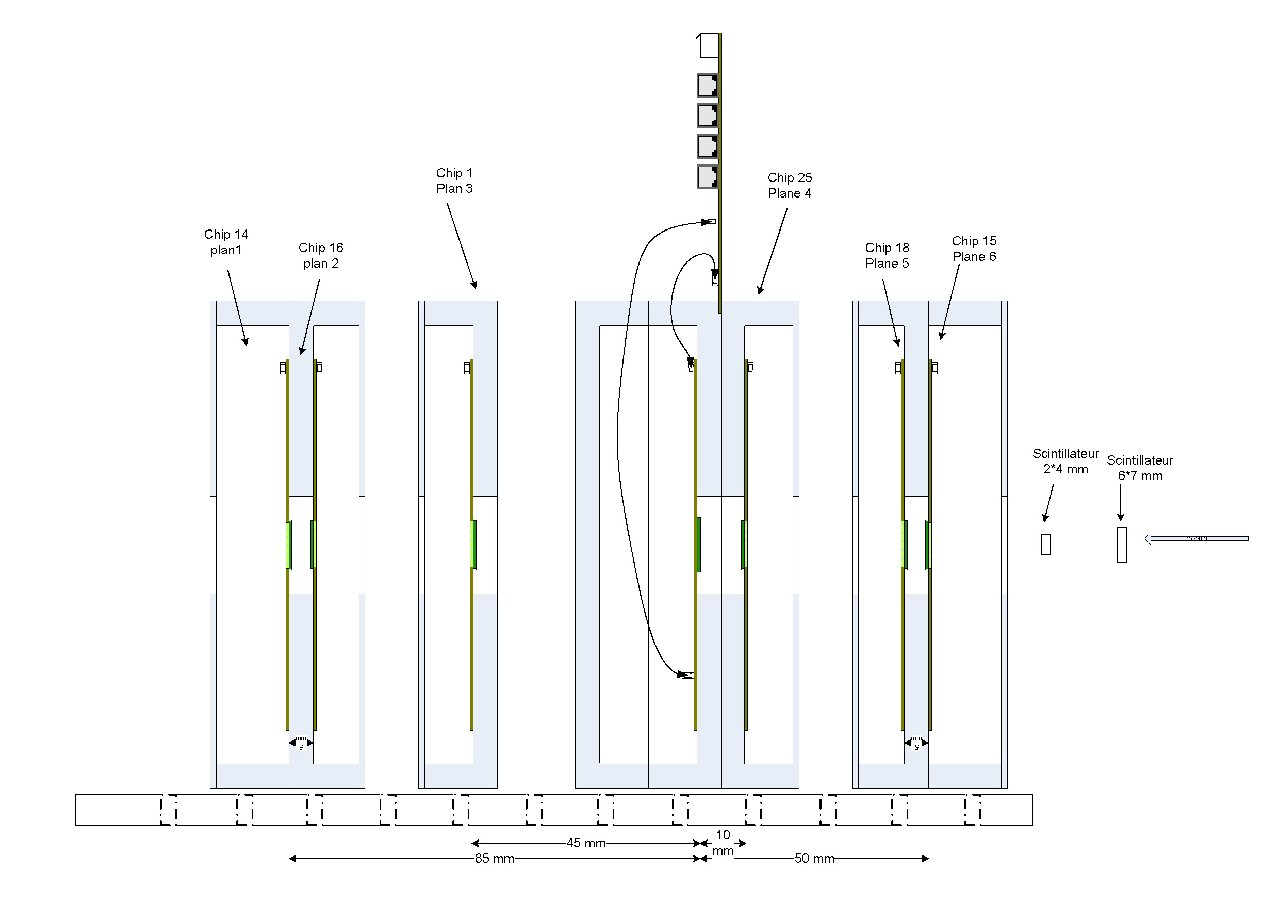
\includegraphics[scale=0.26]{./figures/MIMOSA34/beam_mi34_6plans_Mi26_V3.jpg}
%       \caption{Configuration du t\'elescope V3.}
%      \label{fig:V3}
%      \end{center}
%    \end{figure}
%    
%    \begin{figure}[!Htb]
%      \begin{center} 
%       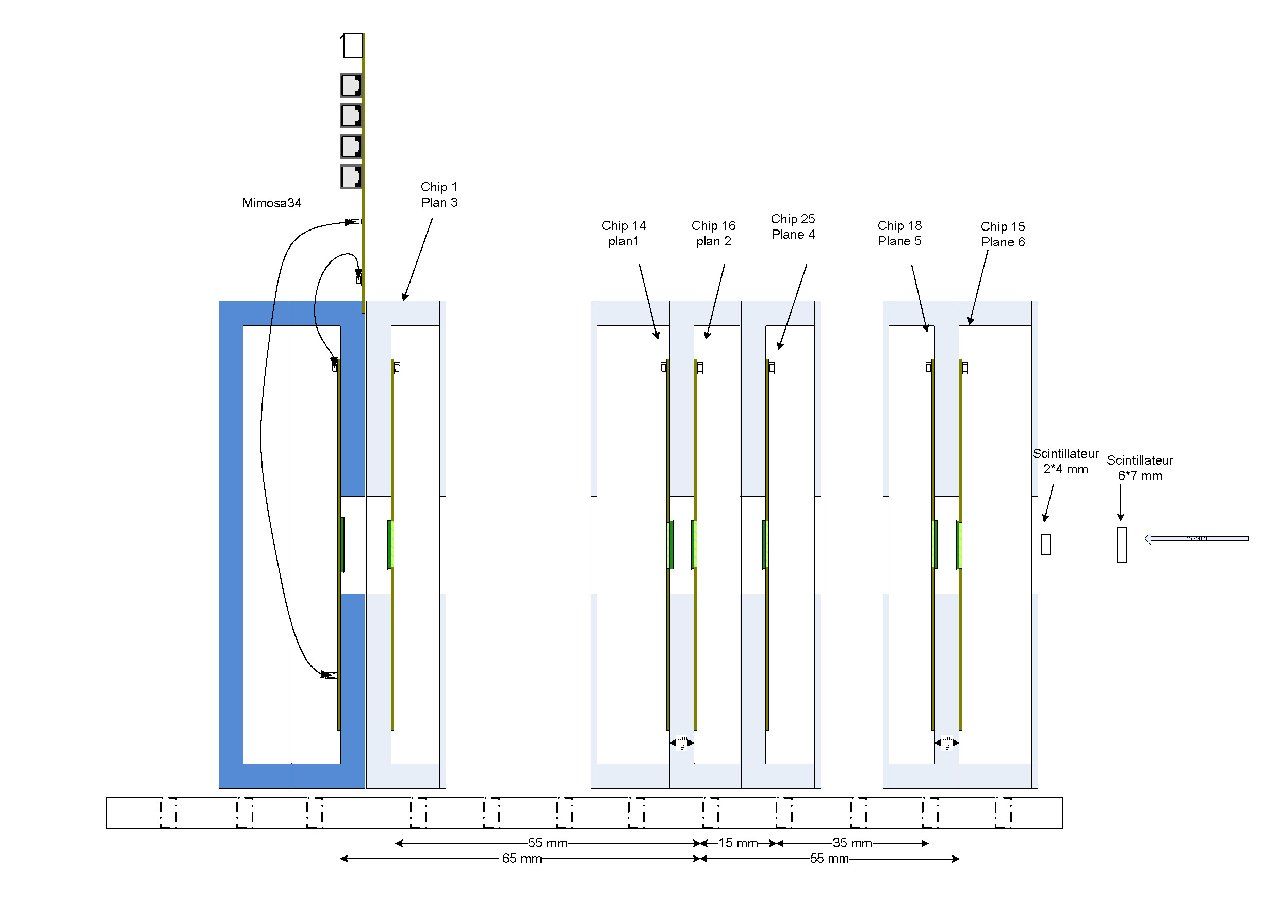
\includegraphics[scale=0.26]{./figures/MIMOSA34/beam_mi34_6plans_Mi26_V4bis.jpg}
%       \caption{Configuration du t\'elescope V4.}
%      \label{fig:V4}
%      \end{center}
%    \end{figure}
%    
%    \medskip
%    
%    Les m\^eme six capteurs ont \'et\'e utilis\'es pour la configuration V4. Ils sont plac\'es \`a $-10 \, mm$, $-60 \, mm$, $-65 \, mm$, $-80 \, mm$, $-115 \, mm$ et $-120 \, mm$ selon l'axe du faisceau avec comme origine le \textit{DUT}. Pour chaque configuration un scintillateur de $8 \times 7 \, mm^2$ est utilis\'e comme d\'eclencheur. Il est plac\'e \`a l'avant du t\'elescope. Les configurations V3 et V4 sont respectivement illustr\'ees en figure \ref{fig:V3} et \ref{fig:V4}.
%    
%    \medskip
%    
%    Pour la simulation des capteurs des t\'elescopes des configurations V3 et V4, des capteurs de type MIMOSA-28 HR15 fonctionnant \`a un seuil de 8 fois la valeur moyenne du bruit ont \'et\'e utilis\'es.  Ceux-ci poss\`edent une r\'esolution spatiale de $3.5 \, \mu m$ et non $4.0 \, \mu m$ comme les capteurs MIMOSA-26 utilis\'es lors des tests. Cela n'emp\^eche pas l'estimation de la diffusion multiple \'etant donn\'e que seul compte le budget de mati\`ere. Or celui-ci est consid\'er\'e identique pour les deux capteurs puisqu'ils ont la m\^eme épaisseur. Dans le but de négliger la r\'esolution du \textit{DUT} dans l'\'equation \ref{eq:resolution2}, le capteur MIMOSA-34 a \'et\'e remplac\'e par un capteur de pas inter-pixel valant $1 \, \mu m$ selon la direction horizontale $U$ et vertical $V$ du capteur. Cela donne une r\'esolution spatiale meilleure que $ \sigma_{DUT} < 1/\sqrt{12} \approx 0.3 \mu m$. La r\'esolution du \textit{DUT} \'elev\'ee au carr\'e est ainsi strictement inf\'erieure \`a $0.1 \, \mu m^2$. On la considérera \'egale \`a $\sigma_{DUT}^2 = 0.1 \mu m^2$. La r\'esolution du t\'elescope avec des traces droites, c'est-\`a-dire avec une impulsion infinie, pour V3 est estim\'ee \`a $1.8 \, \mu m$ et celle pour V4 \`a $3.5 \, \mu m$ gr\^ace \`a la relation \ref{eq:propag_erreurs}. Un faisceau d'\'electrons parall\`ele \`a l'axe du t\'elescope ($Oz$) et d'impulsion variable est utilis\'e. Chaque plan des configurations V3 et V4 est plac\'e perpendiculairement au faisceau (imagin\'e sans diffusion multiple.) selon les positions indiqu\'ees plus haut.
%    
%    \subsection{R\'esultats}
%    
%    Nous allons \`a pr\'esent exposer les r\'esultats obtenus avec ces deux configurations. Puis, nous en tirerons une estimation du terme $\sigma_{ms}$ de la relation \ref{eq:resolution2}. Pour la configuration V3, la figure \ref{fig:res_vs_energy_V3} indique la valeur de la largeur de la distribution des r\'esidus sur le \textit{DUT} en fonction de l'impulsion du faisceau d'\'electrons. En premi\`ere approximation, c'est \`a dire en n\'egligeant la r\'esolution spatiale du DUT, on a :
% 
%    \begin{equation}
%     \sigma_{Res} = \sqrt{\sigma_{Tel}^2 + \sigma_{ms}^2}
%     \label{eq:sigma_ms}
%    \end{equation}
%    
%    Comme la diffusion multiple est proportionnelle \`a $1/p$, on peut \'ecrire : 
%    
%    \begin{equation}
%     \sigma_{Res} = \sigma_{Tel} \sqrt{ 1 + \dfrac{C}{p^2 \sigma_{Tel}^2} }
%    \end{equation}
%    
%    Avec le terme $\sigma_{Tel}$ constant et valant 1.8 $\mu m$ pour V3 ($3.5 \, \mu m$ pour V4) et $C$ une constante. On s'attend donc \`a observer une courbe tendant vers l'infinie en 0 et d\'ecroissant vers une asymptote horizontale \'egale \`a la valeur de $\sigma_{Tel}$. C'est ce qu'on observe sur la figure \ref{fig:res_vs_energy_V3}.
%    
%    \begin{figure}[!Htb]
%      \begin{center} 
%       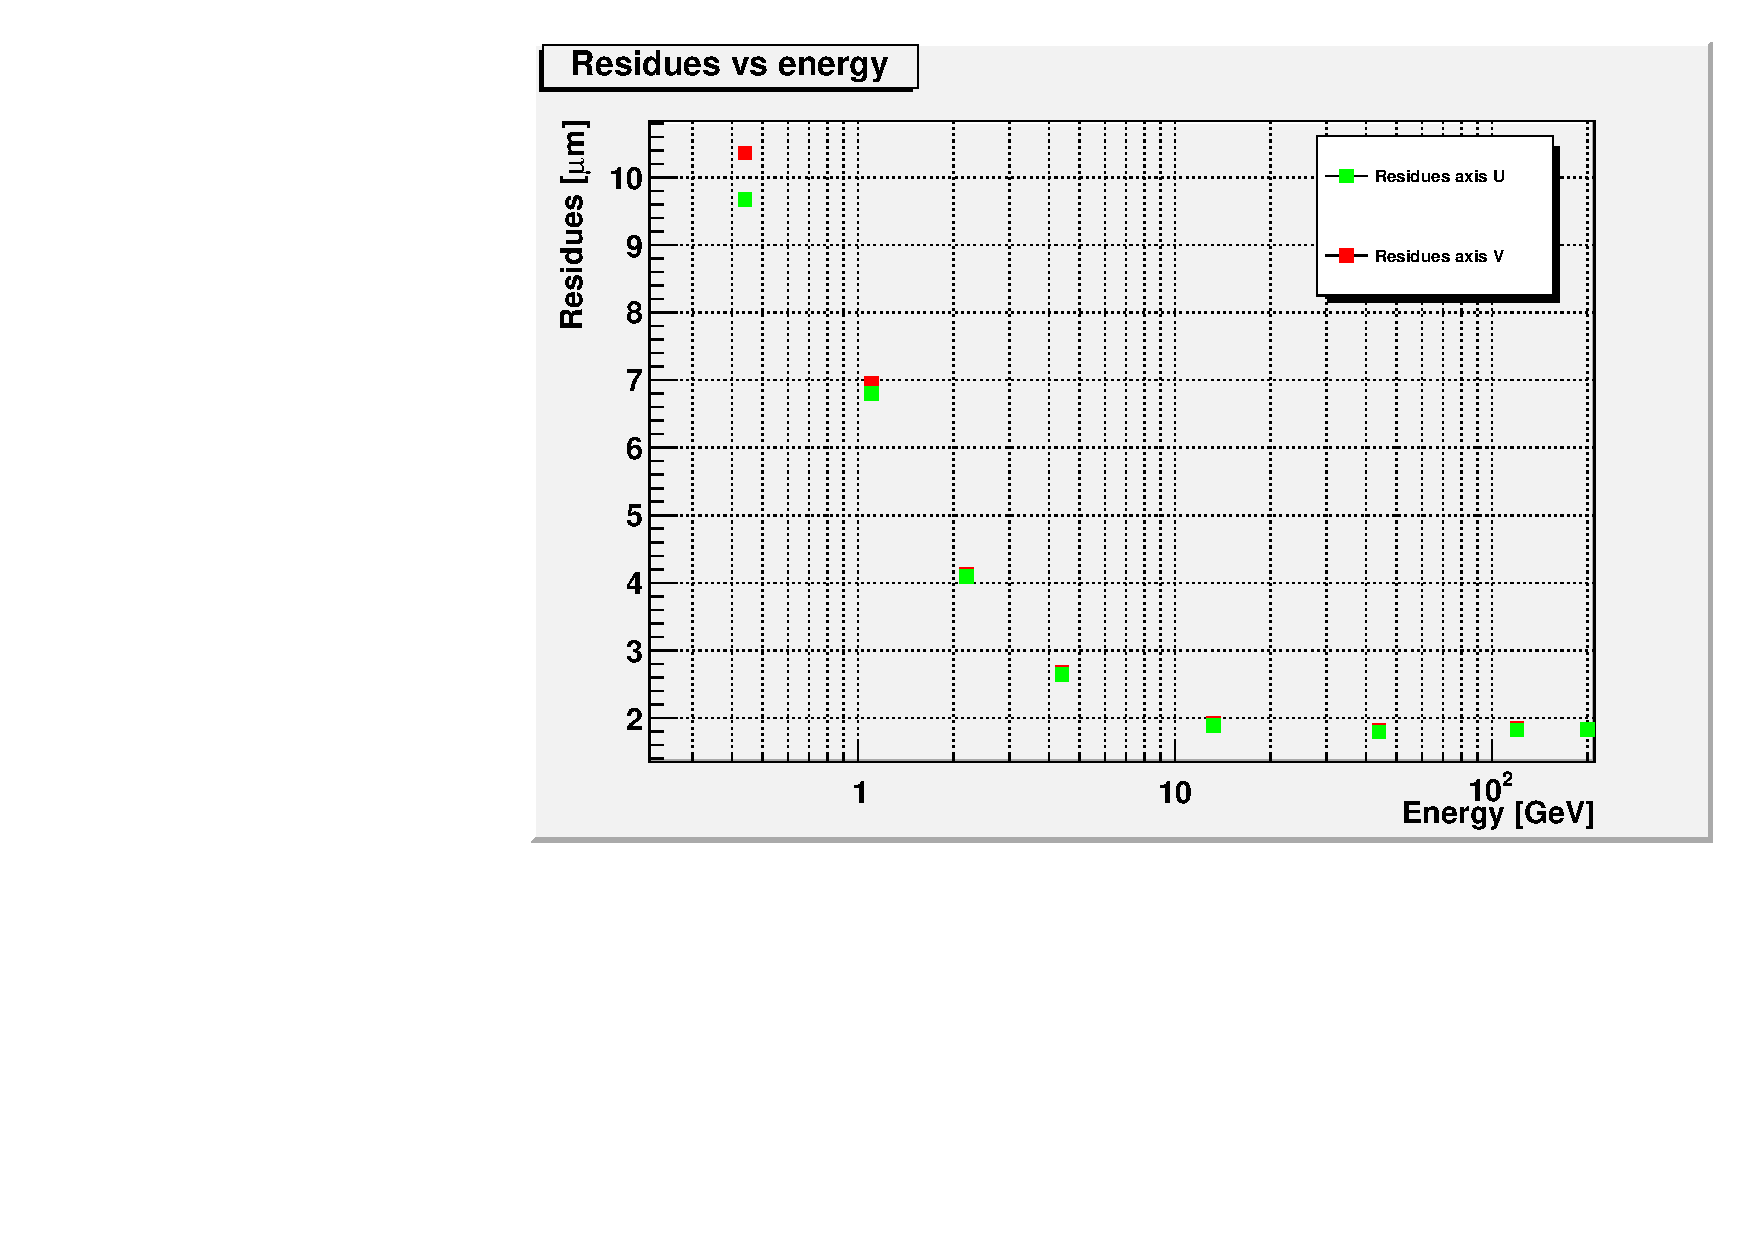
\includegraphics[scale=0.60]{./figures/MIMOSA34/residues_vs_energy_V3.pdf}
%       \caption{Largeur de la distribution des r\'esidus selon les axes $U$ et $V$ du \textit{DUT} pour la configuration V3 en fonction de l'impulsion du faisceau de particules.}
%      \label{fig:res_vs_energy_V3}
%      \end{center}
%    \end{figure}
%    
%    \`A 0.44 $GeV/c$ la largeur des r\'esidus vaut environ 10 $\mu m$, puis celle-ci diminue jusqu'\`a la valeur th\'eorique attendue de 1.8 $\mu m$. \`A 4.4 $GeV/c$, l'\'energie de l'exp\'erience \`a DESY, la largeur pour la distribution des r\'esidus vaut $2.64 \pm 0.02 \, \mu m$.
%    
%    \medskip
%    
%    La figure \ref{fig:res_vs_chi2_V3} repr\'esente la largeur de la distribution des r\'esidus obtenue en fonction de diff\'erentes coupures sur le $\chi^2$ des traces pour une impulsion des \'electrons de $4.4 \, GeV$. La coupure en $\chi^2$ selon un certain seuil s\'electionne les traces dont l'ajustement est d'assez bonne qualit\'e pour donner un $\chi^2$ inf\'erieur \`a la limite consid\'er\'ee. La diffusion multiple implique des traces non droites. Cela influe sur la qualit\'e de l'ajustement du mod\`ele de trace droite. Autrement dit, la diffusion multiple d\'egrade la qualit\'e de l'ajustement et donc le $\chi^2$ des traces. Ainsi, si la reconnaissance des coups appartenant \`a la vraie trace est parfaite, plus le $\chi^2$ de la trace est faible, plus la diffusion multiple aura jou\'e un faible r\^ole. Le but d'une telle coupure est d'observer et de comparer avec les donn\'ees des tests en faisceau l'influence de la coupure en $\chi^2$ sur les traces. On notera que plus la coupure en $\chi^2$ est importante (faibles valeurs de $\chi^2$) plus les traces sont droites et plus l'alignement est facilit\'e. Pour la configuration V3, la valeur de la largeur de la distribution des r\'esidus passe de $2.65 \, \mu m$ pour un $\chi^2 \leq 100$ \`a une valeur d'environ $2.35$ \`a $2.40 \, \mu m$ pour un $\chi^2 \leq 0.5$. La coupure en $\chi^2$ commence \`a se faire sentir \`a partir des valeurs de $\chi^2$ inf\'erieures \`a 10.
%    
%    \begin{figure}[!Hbt]
%      \begin{center}
%       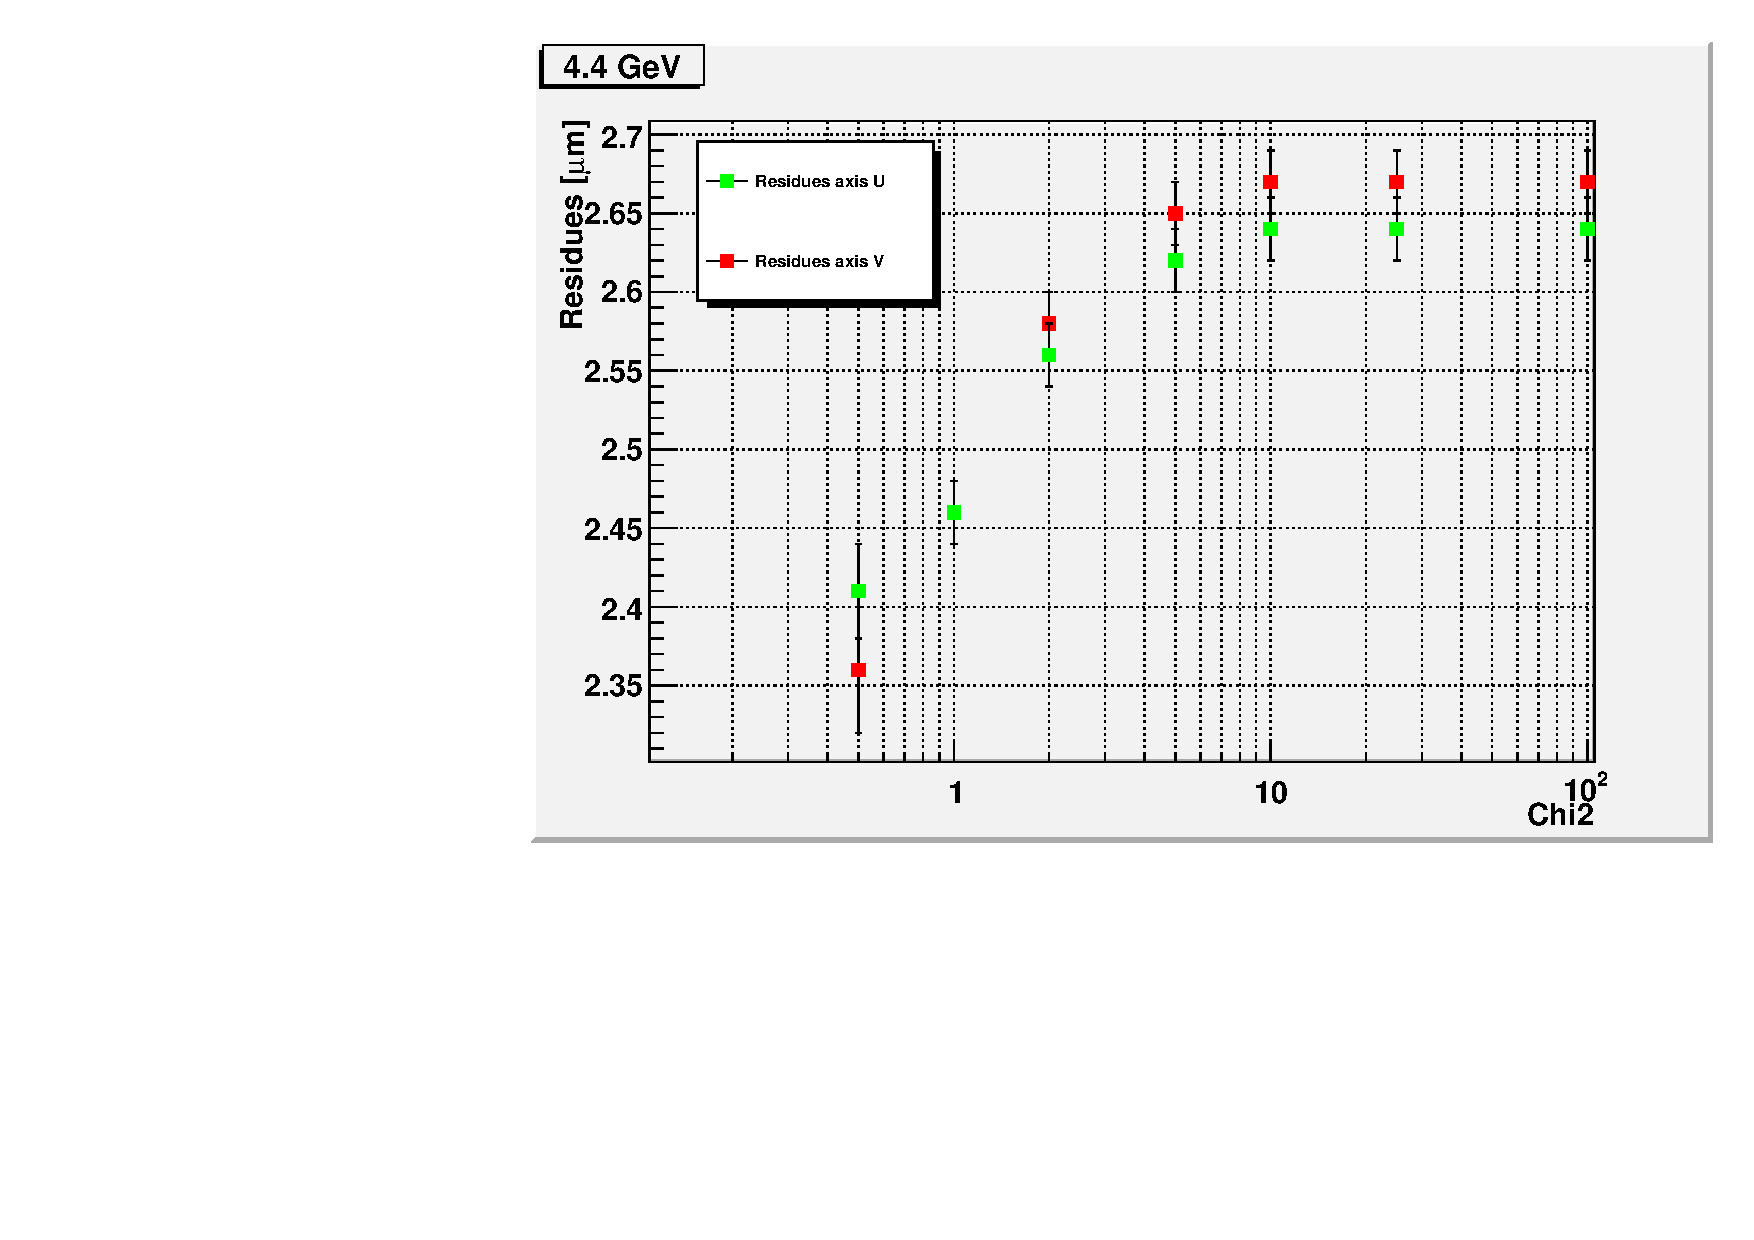
\includegraphics[scale=0.60]{./figures/MIMOSA34/residues_vs_chi2_4-4GeV_V3.pdf}
%       \caption{Largeur de la distribution des r\'esidus selon les axes $U$ et $V$ du \textit{DUT} pour la configuration V3 \`a 4.4 $GeV/c$ en fonction de la coupure en $\chi^2$ des traces.}
%      \label{fig:res_vs_chi2_V3}
%      \end{center}
%    \end{figure}
%   
%    \begin{figure}[!Htb]
%      \begin{center} 
%       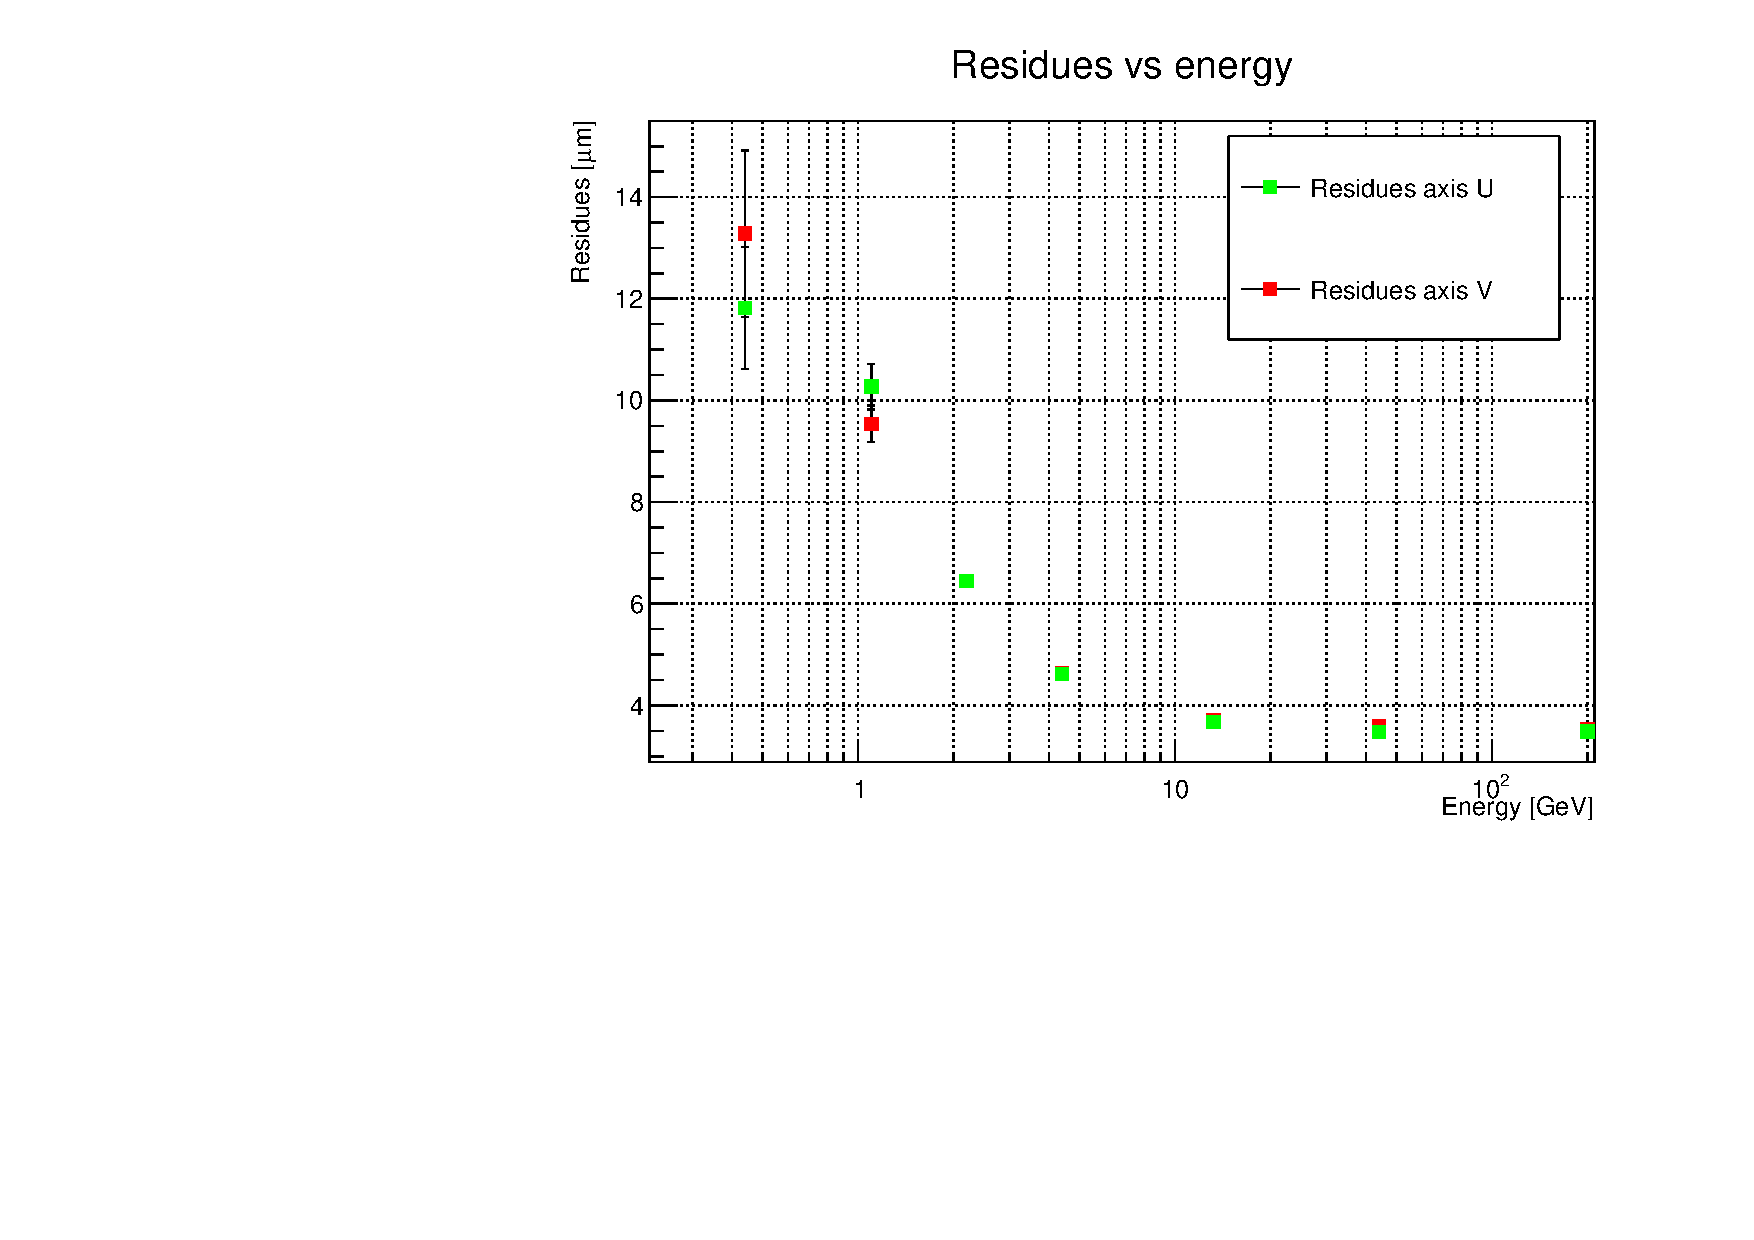
\includegraphics[scale=0.60]{./figures/MIMOSA34/residues_vs_energy_V4.pdf}
%       \caption{Largeur de la distribution des r\'esidus selon les axes U et V pour la configuration V4 en fonction de l'impulsion du faisceau de particules.}
%      \label{fig:res_vs_energy_V4}
%      \end{center}
%    \end{figure}
% 
%    \begin{figure}[!Htb]
%      \begin{center} 
%       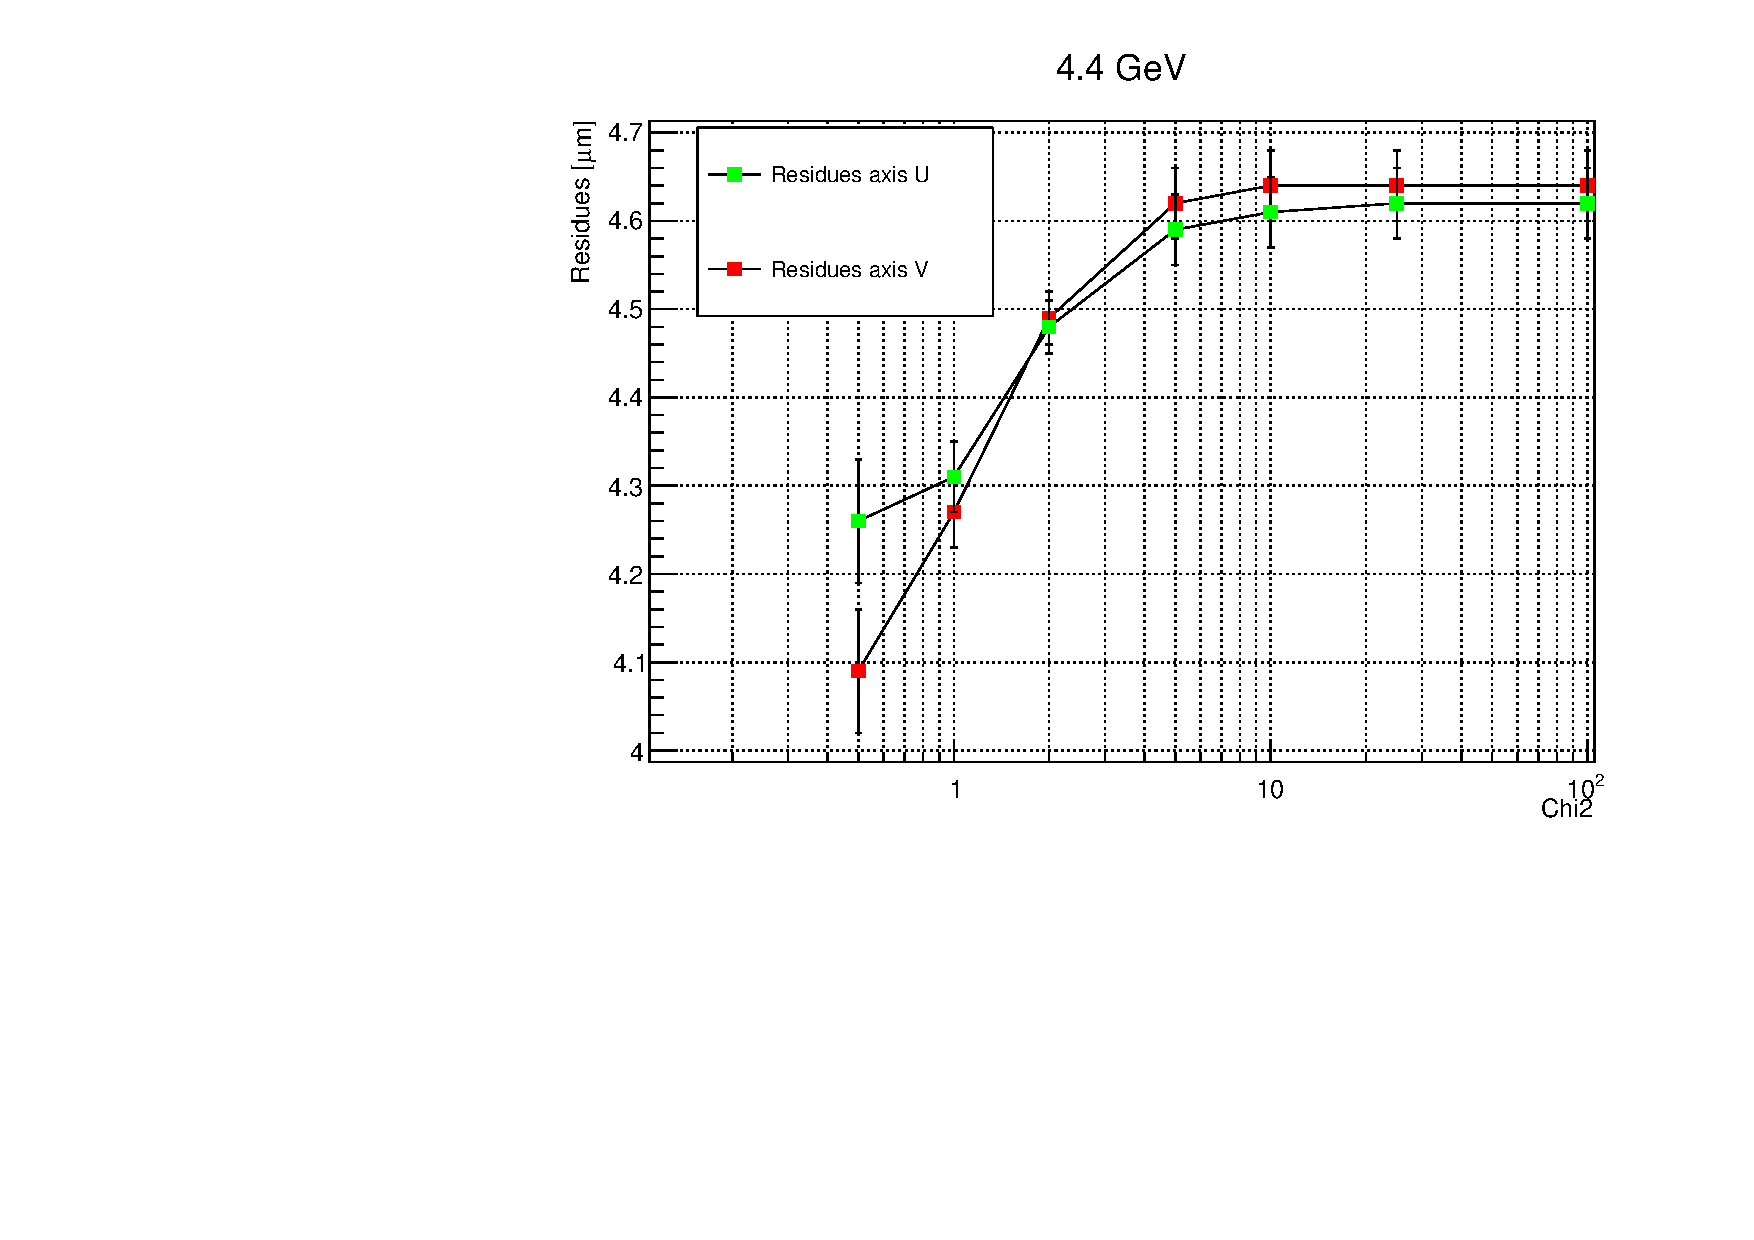
\includegraphics[scale=0.60]{./figures/MIMOSA34/residues_vs_chi2_4-4GeV.pdf}
%       \caption{Largeur de la distribution des r\'esidus selon les axes U et V pour la configuration V4 \`a 4.4 $GeV/c$ en fonction de la coupure en $\chi^2$ des traces.}
%      \label{fig:res_vs_chi2_V4}
%      \end{center}
%    \end{figure} 
% 
%    \medskip
%    
%    Pour la configuration V4, la figure \ref{fig:res_vs_energy_V4} repr\'esente la largeur de la distribution des r\'esidus sur le \textit{DUT} en fonction de l'impulsion du faisceau de particules. Cette largeur diminue progressivement en passant de respectivement 12 \`a 13 $\mu m$ pour les axes $U$ et $V$ du \textit{DUT} \`a 0.44 $GeV/c$ \`a 3.5 $\mu m$ pour une impulsion de 200 $GeV/c$. La valeur de $3.5 \, \mu m$ est bien obtenue comme attendue \`a haute impulsion. Pour une impulsion de 4.4 $GeV/c$ correspondante aux tests en faisceau \`a DESY, et pour la configuration V4, la valeur de la largeur des r\'esidus s'\'etablie \`a $4.62 \pm 0.04$ $\mu m$. 
%    
%    \medskip
%    
%    La figure \ref{fig:res_vs_chi2_V4} repr\'esente quant \`a elle la largeur de la distribution des r\'esidus en fonction de la coupure en $\chi^2$ sur les traces. Pour la configuration V4, la valeur de la largeur de la distribution des r\'esidus passe de $4.62 \mu m$ pour un $\chi^2 \leq 100$ \`a une valeur d'environ $4.1 \mu m$ pour un $\chi^2 \leq 0.5$. La coupure en $\chi^2$ commence \`a se faire ressentir \`a partir des valeurs de $\chi^2$ inf\'erieures \`a 10.
%    
%    \medskip
%    
%    En prenant en compte une coupure sur le $\chi^2$ des traces sup\'erieures \`a 10, la largeur de la distribution des r\'esidus sur le \textit{DUT} pour un faisceau d'\'electrons dot\'es d'une impulsion de 4.4 $GeV/c$ vaut environ 2.65 $\mu m$ pour la configuration V3 et 4.6 $\mu m$ pour la configuration V4. Selon l'équation approch\'ee \ref{eq:sigma_ms}, les valeurs de $\sigma_{ms}$ sont estim\'ees \`a environ $1.95 \, \mu m$ pour la configuration V3 et \`a $3.00 \, \mu m$ pour la configuration V4. En utilisant les valeurs de $\sigma_{ms}$ obtenues avec cette \'etude, les r\'esolutions calcul\'ees sur les diff\'erentes matrices de pixels de MIMOSA34 sont encore trop \'elev\'ees compar\'ees aux pr\'evisions th\'eoriques. Cela est notamment le cas pour la configuration V3 et est moins vrai pour la configuration V4. Ces r\'esultats nous am\`enent donc \`a penser que les t\'elescopes dans leurs configurations V4 mais surtout V3 ont \'et\'e mal align\'es lors de l'analyse hors ligne. En cause, la diffusion multiple, rendant difficile l'ajustement de traces droites. Avec notre simulation, diff\'erents d\'esalignements ont \'et\'e effectu\'es sur les configurations V3 et V4, et ont montr\'e qu'en cas de d\'esalignement des plans du t\'elescope, la largeur de la distribution des r\'esidus augmente. A l'heure de l'\'ecriture de ce rapport, les analyses concernant MIMOSA-34 sont encore en cours.
%   // END


%   
%   \chapter{Efficacit\'e de reconstruction des mini-vecteurs}
%   
%   L'efficacit\'e de reconstruction a \'et\'e \'evalu\'ee en comparant les pentes et les positions des mini-vecteurs avec les donn\'ees Monte Carlo.
%   
%   \medskip
%   
%   Les mini-vecteurs sont exprim\'es par un vecteur directeur $\overrightarrow{v_{MV}} = (R_X, R_Y, 1.0)$ et un point $P(P_X,P_Y,P_Z)$ correspondant \`a leur milieu dans le rep\`ere du laboratoire. Le vecteur directeur de la trace Monte Carlo \`a l'origine du mini-vecteur est not\'e $\overrightarrow{v_{MC}} = (V_X, V_Y, 1.0)$ et le point d'origine de la trace $T(T_X,T_Y,T_Z)$. Pour \'evaluer le mini-vecteur reconstruit nous allons comparer les pentes et l'origine de la trace avec la projection du mini-vecteur \`a la m\^eme coordonn\'ee $Z$ que l'origine de la trace. Les coordonn\'ees du vecteur directeur d'un mini-vecteur prennent les valeurs des tangentes suivantes :
%   
%   \begin{equation}
%    R_X = \tan(\theta_x) = \cfrac{L_x}{2090}
%   \end{equation}
% 
%   \begin{equation}
%    R_Y = \tan(\theta_y) = \cfrac{L_y}{2090}
%   \end{equation}
%   
%   \begin{figure}[!htb]
%     \begin{center}
%       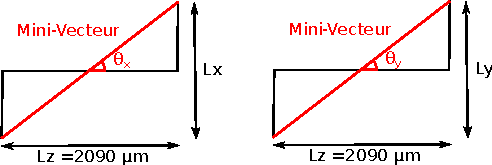
\includegraphics[scale=1.5]{./figures/angle_trace_MV.pdf}
%       \caption{Angles des mini-vecteurs.}
%       \label{fig:tan_MV}
%     \end{center}
%   \end{figure}
%   
%   O\`u $L_x$ et $L_y$ correspondent aux longueurs du mini-vecteur selon les axes $X$ et $Y$ comme illustr\'e en figure \ref{fig:tan_MV}. Afin de rendre compte des erreurs sur les pentes $R_X$ et $R_Y$ de chaque mini-vecteur, dues aux erreurs sur les deux points de reconstruction du mini-vecteur, on d\'efinit une valeur de pente minimale et une valeur de pente maximale pour chacune des deux pentes de chaque mini-vecteur. Ces valeurs minimales et maximales sont calcul\'ees en ajoutant ou en soustrayant $N$ fois la r\'esolution spatiale aux valeurs $L_x$ et $L_y$. Les valeurs $L_x^{max/min}  = L_x \pm 2 \times N \times \sigma_{capteur}$ et $L_y^{max/min}  = L_y \pm 2 \times N \times \sigma_{capteur}$ correspondent aux erreurs extr\^emes sur chacun des axes de chaque face. Les valeurs des pentes minimales et maximales des mini-vecteurs correspondantes sont ensuite compar\'ees aux valeurs $V_X$ et $V_Y$ des pentes des traces Monte Carlo passant \`a travers l'\'echelle. Si l'une des pentes de la trace Monte-Carlo d\'epasse les limites de pentes des mini-vecteurs, le mini-vecteur est consid\'er\'e comme mal reconstruit.  Sinon il est \'etiqueté comme bien reconstruit jusqu'au test suivant. La valeur de $N = 3$, correspondant \`a un intervalle de confiance de $99.7 \, \%$ a \'et\'e choisie dans la suite. La valeur de la r\'esolution spatiale $\sigma_{capteur}$ a \'et\'e choisie en fonction de l'inclinaison de la trace. La valeur de $3.5 \, \mu m$ a \'et\'e prise \`a incidence normale.
%   
%   \medskip
%   
%   Un autre test permet de s'assurer de la bonne localisation du mini-vecteur \'etudi\'e. On projette alors chaque mini-vecteur en $Z=0$. Comme la position initiale des traces Monte Carlo en $Z=0$ est connue, on peut comparer le point de la trace Monte Carlo en $Z=0$  avec la projection du mini-vecteur en $Z=0$. Une diff\'erence des coordonn\'ees selon les axes $X$ et $Y$ est alors r\'ealis\'ee. Les deux distances obtenues, selon $X$ et $Y$ sont ensuite compar\'ees \`a une distance limite correspondant \`a la projection du mini-vecteur avec sa limite de pente inf\'erieure ou sup\'erieure. Calculons la distance limite selon $X$ et selon la configuration donn\'ee en figure \ref{fig:ConfigRecoMVs} :
%   
%   \begin{equation}
%    \tan(\theta_{x(y)}) = \cfrac{d_{y(x)}}{30000} = \cfrac{ L_{y(x)} + 2 \times N \times \sigma_{capteur}}{2090}
%   \end{equation}
%   
%   Ce qui nous donne :
%   
%   \begin{equation}
%    d_{y(x)} = \cfrac{30 000}{2090} \times \left( 2 \times N \times \sigma_{capteur} \right)
%   \end{equation}
%   
%   La distance $d_x$ est calcul\'ee de la même fa\c{c}on. A incidence normale et pour $N = 3$ on a $d = d_x = d_y = \approx 302 \, \mu m$. Les distances entre la projection du mini-vecteur et le point de la trace Monte Carlo ne doivent pas d\'epasser les distances respectives $d_x$ et $d_y$. Si les distances obtenues d\'epassent l'une des deux distances limites, le mini-vecteur est consid\'er\'ee comme mal reconstruit. Les mini-vecteurs pointant \`a l'int\'erieur de la zone limite, sont consid\'er\'es comme bien reconstruits s'ils ont aussi pass\'e le premier test sur leurs pentes.
%   
%   \medskip
%   
%   \begin{figure}[!htb]
%     \begin{center}
%       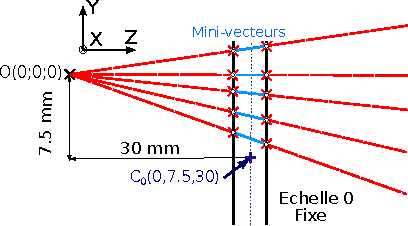
\includegraphics[scale=1.8]{./figures/reconstructionMV.pdf}
%       \caption{Sch\'ema de la configuration utilis\'ee pour l'analyse de la reconstruction des mini-vecteurs. Les mini-vecteurs sont reconstruits sur l'\'echelle 0. Les traces sont visibles en rouge et les mini-vecteurs en bleu.}
%       \label{fig:ConfigRecoMVs}
%     \end{center}
%   \end{figure}
%   
%   Nous allons \`a pr\'esent \'evaluer l'efficacit\'e de reconstruction avec la configuration illustr\'ee en figure \ref{fig:ConfigRecoMVs}. Avec cette configuration nous utilisons des pions n\'egatifs dot\'es d'une impulsion de 120 $GeV/c$. Ceux-ci sont distribu\'es al\'eatoirement sur une ligne de $10 \, cm$ parall\`ele \`a l'axe $Ox$ et centr\'ee en $O(0,0,0)$ et ils sont envoy\'es en direction de l'\'echelle avec des angles selon les axes $Ox$ et $Oy$ pris dans l'intervalle $[-15, 15]$ degr\'es. La direction de chaque pions est tir\'ee dans une distribution uniforme. Ainsi, la densit\'e de mini-vecteurs sur la surface de l'\'echelle sera homog\`ene (pour un grand nombre de mini-vecteurs reconstruits).
%   
%   \begin{figure}[!htb]
%     \begin{center}
%       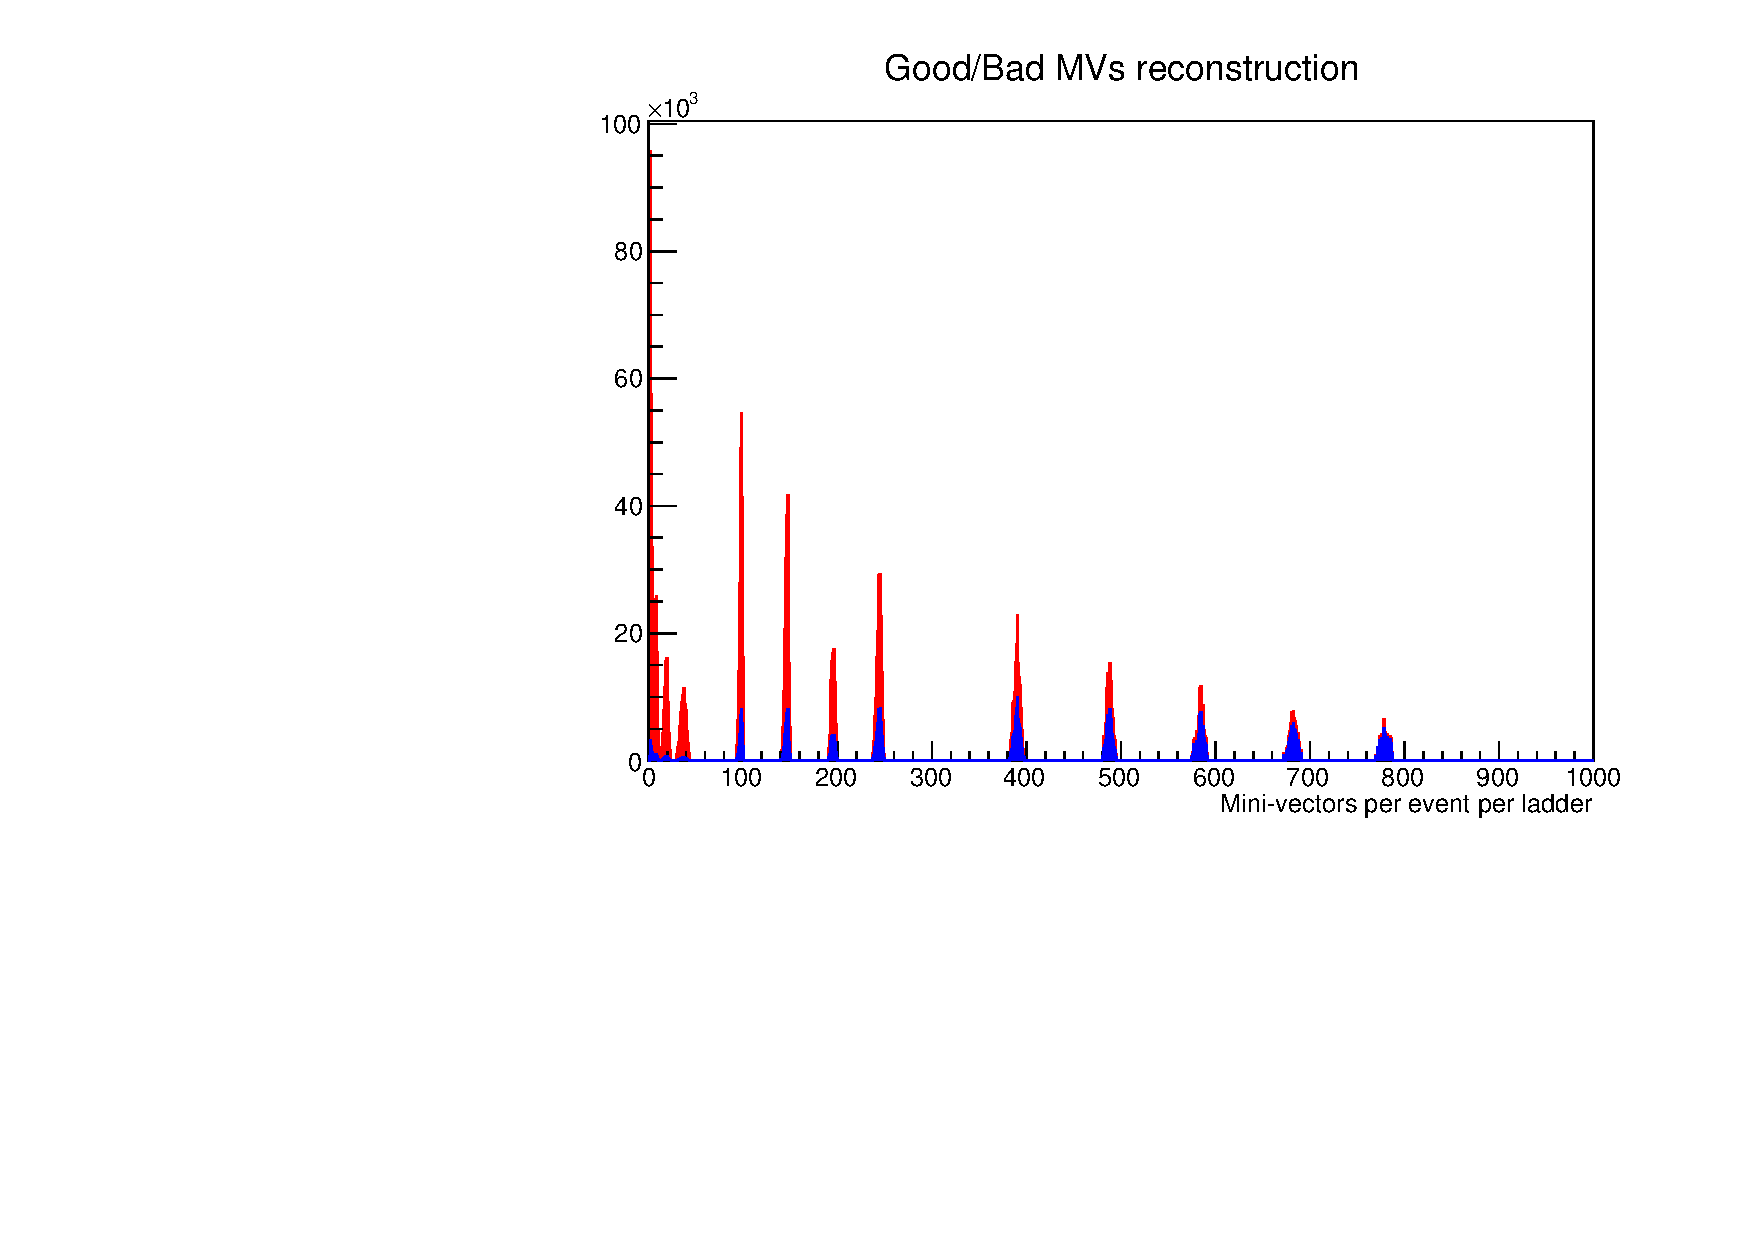
\includegraphics[scale=0.55]{./figures/EffMVs/efficiencyMiniVectorStudies/efficiencyNew/GoddBadMVs.pdf}
%       \caption{Reconstruction des mini-vecteurs en fonction du nombre de mini-vecteurs reconstruits par \'ev\'enement sur l'\'echelle 0. En rouge sont indiqu\'es les bonnes associations et en bleu les mauvaises associations.}
%       \label{fig:goodBadMVs}
%     \end{center}
%   \end{figure}
%   
%   \begin{figure}[!htb]
%     \begin{center}
%       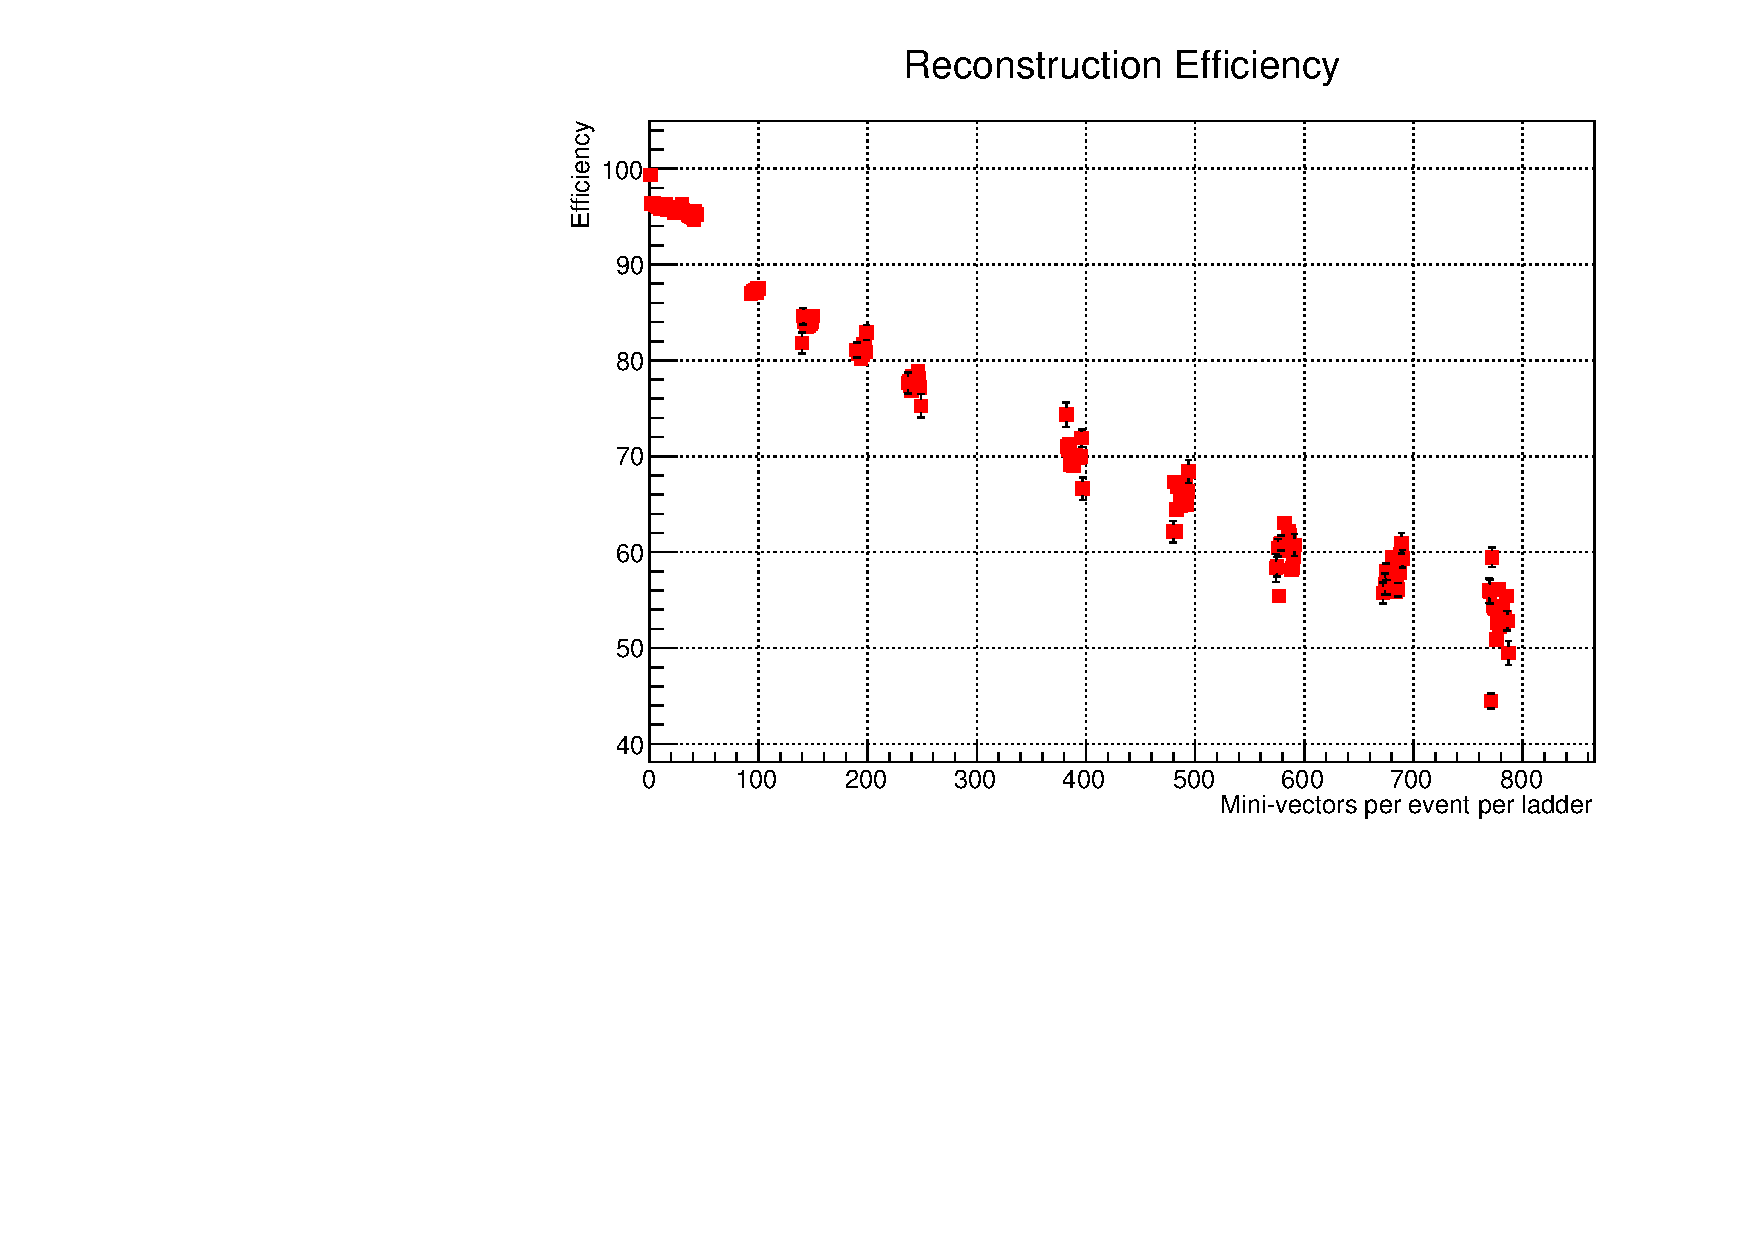
\includegraphics[scale=0.55]{./figures/EffMVs/efficiencyMiniVectorStudies/efficiencyNew/reconstructionEfficiency.pdf}
%       \caption{Efficacit\'e de reconstruction des mini-vecteurs en fonction du nombre de mini-vecteurs reconstruits par \'ev\'enement sur l'\'echelle 0.}
%       \label{fig:effReconstruction}
%     \end{center}
%   \end{figure}
% 
%   \begin{figure}[!htb]
%     \begin{center}
%       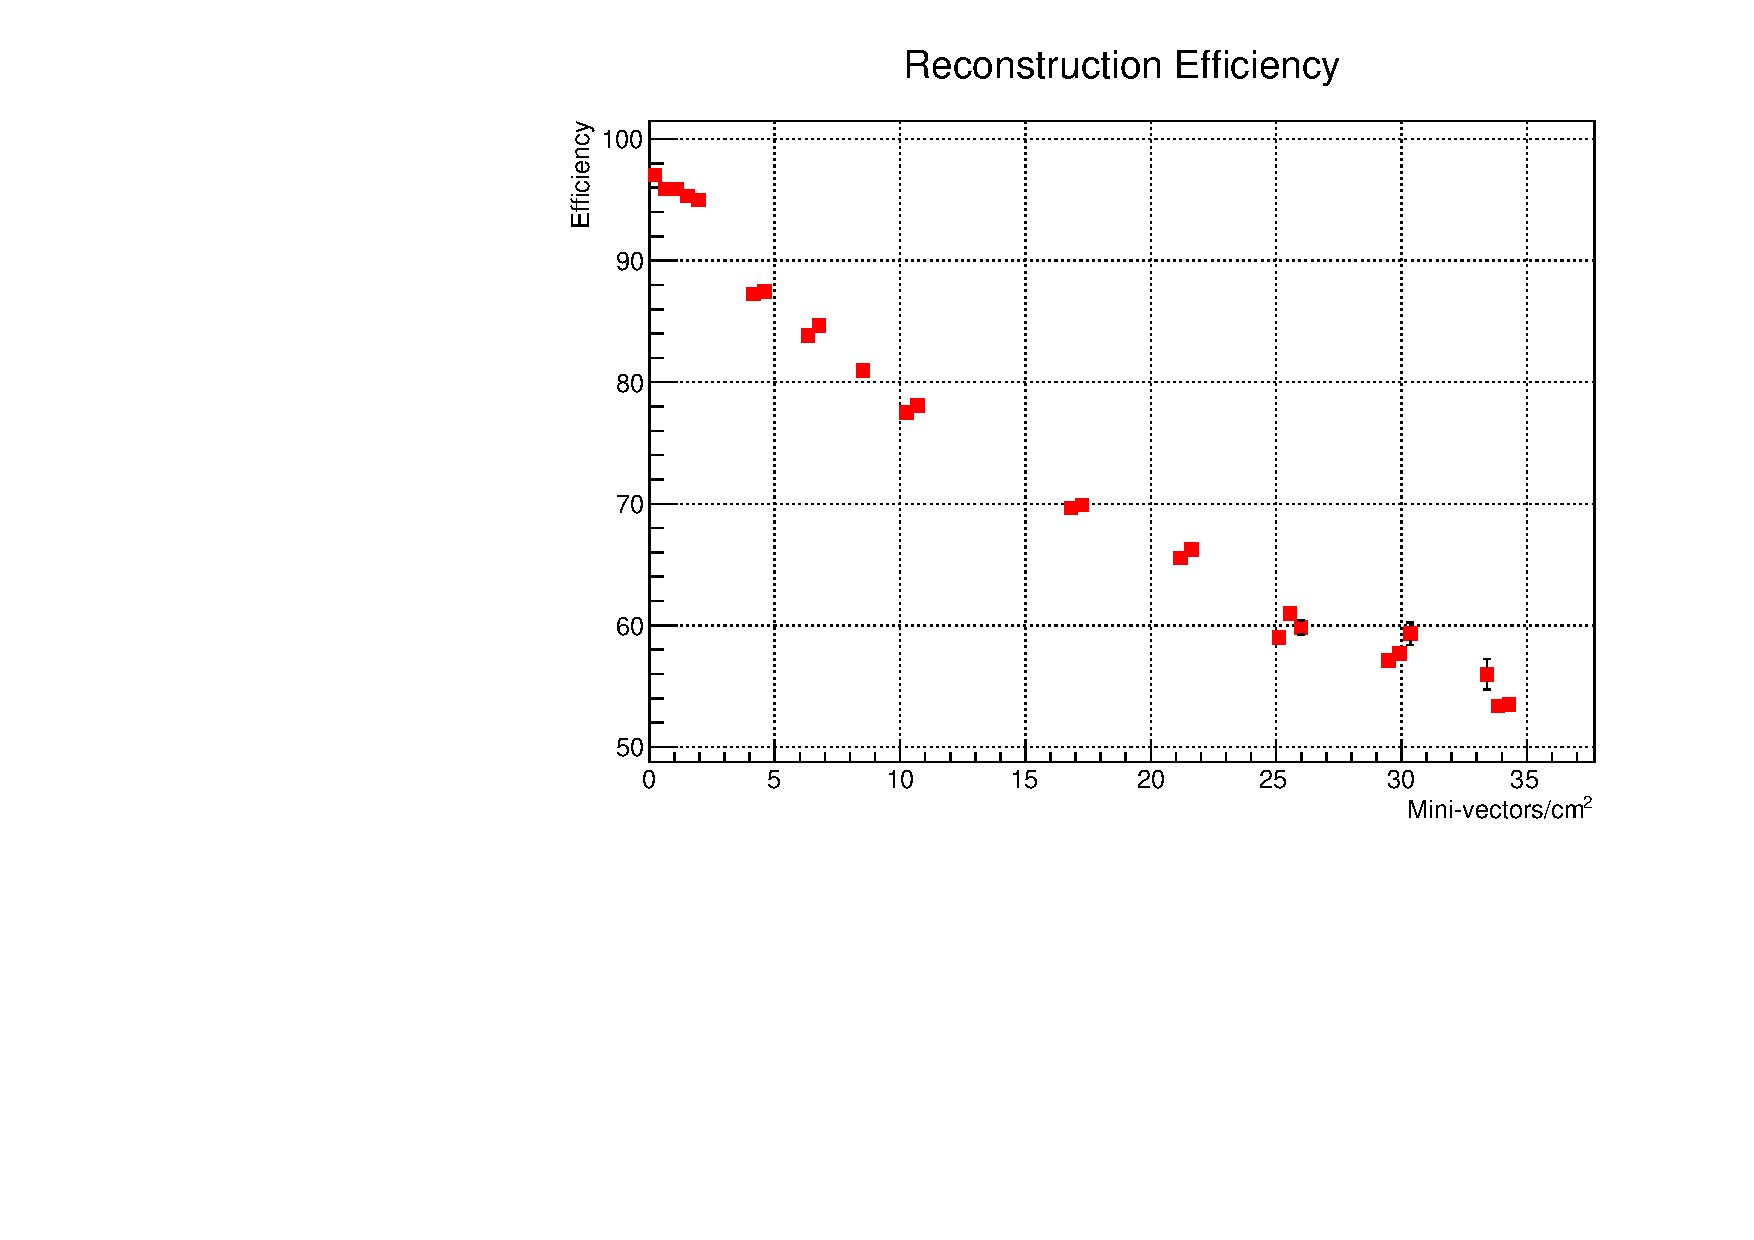
\includegraphics[scale=0.55]{./figures/EffMVs/efficiencyMiniVectorStudies/efficiencyNew/reconstructionEfficiencyDensity.pdf}
%       \caption{Efficacit\'e de reconstruction des mini-vecteurs en fonction de la densit\'e de mini-vecteurs reconstruits par \'ev\'enement (en mini-vecteurs/$cm^2$).}
%       \label{fig:effReconstructionDensity}
%     \end{center}
%   \end{figure}
% 
%   \medskip
%   
%   La figure \ref{fig:goodBadMVs} montre les bonnes et les mauvaises reconstructions de mini-vecteurs en fonction du nombre de mini-vecteurs reconstruits par \'ev\'enement. La figure \ref{fig:effReconstruction} indique les efficacit\'es de reconstruction, \`a partir des donn\'ees de la figure \ref{fig:goodBadMVs}, en fonction du nombre de mini-vecteurs reconstruits par \'ev\'enement sur l'\'echelle 0. Avec une trace par \'ev\'enement, l'efficacit\'e de reconstruction des mini-vecteurs vaut $99.4 \, \%$ . Plus le nombre de traces par \'ev\'enement est grand, plus l'association est difficile et plus l'efficacit\'e de reconstruction diminue. 
%   
%   \medskip
%   
%   On notera que la reconstruction d\'epend de la densit\'e d'impact sur chacune des faces des \'echelles. Plus la densit\'e d'impacts est \'elev\'ee plus la reconstruction est difficile. Pour environ 780 mini-vecteurs par \'ev\'enement on obtient une efficacit\'e de reconstruction de l'ordre de $50 \%$. Les fluctuations de l'efficacit\'e entre des nombres similaires de mini-vecteurs par \'ev\'enement s'explique par la r\'epartition al\'eatoire des param\`etres des traces. En effet, les densit\'es locales d'impacts varient l\'eg\`erement d'un \'ev\'enement \`a un autre. 
%   
%   \medskip
%   
%   La figure \ref{fig:effReconstructionDensity} indique les m\^emes efficacit\'es de reconstruction de mini-vecteur en fonction de la densit\'e d'impact sur l'\'echelle 0. Pour r\'ealiser cette figure, les valeurs d'efficacit\'e ont \'et\'e moyenn\'ees par groupe de 10 mini-vecteurs et le nombre de mini-vecteurs reconstruits sur l'échelle 0 par \'ev\'enement a \'et\'e divis\'e par la surface totale des 6 six capteurs de l'une des faces de l'\'echelle. Cette surface vaut $22.90 \, cm^2$. L'efficacit\'e varie de $97\%$ pour une densit\'e de mini-vecteurs par $cm^2$ inf\'erieure \`a 1 \`a environ $53\%$ pour une densit\'e de 34 mini-vecteurs par $cm^2$.

\chapter{Resultats d'alignement avec une g\'eom\'etrie de la double couche 3}
\label{resultats_align_DL3}

  
  \begin{figure}[htb!]
     \begin{center}
       \subfigure[\'Ecart \`a la valeur Monte-Carlo de la valeur moyenne de la distribution du param\`etre $X1$ apr\`es alignement, en fonction de la statistique. En vert et bleu : $\pm$ une et trois fois largeur de la distribution de ce param\`etre, en fonction de la statistique. A titre indicatif, les lignes rouges repr\'esente les valeurs de $\pm 1 \mu m$.]{
         \label{fig:MV_prec_Axe_X_DL3}
         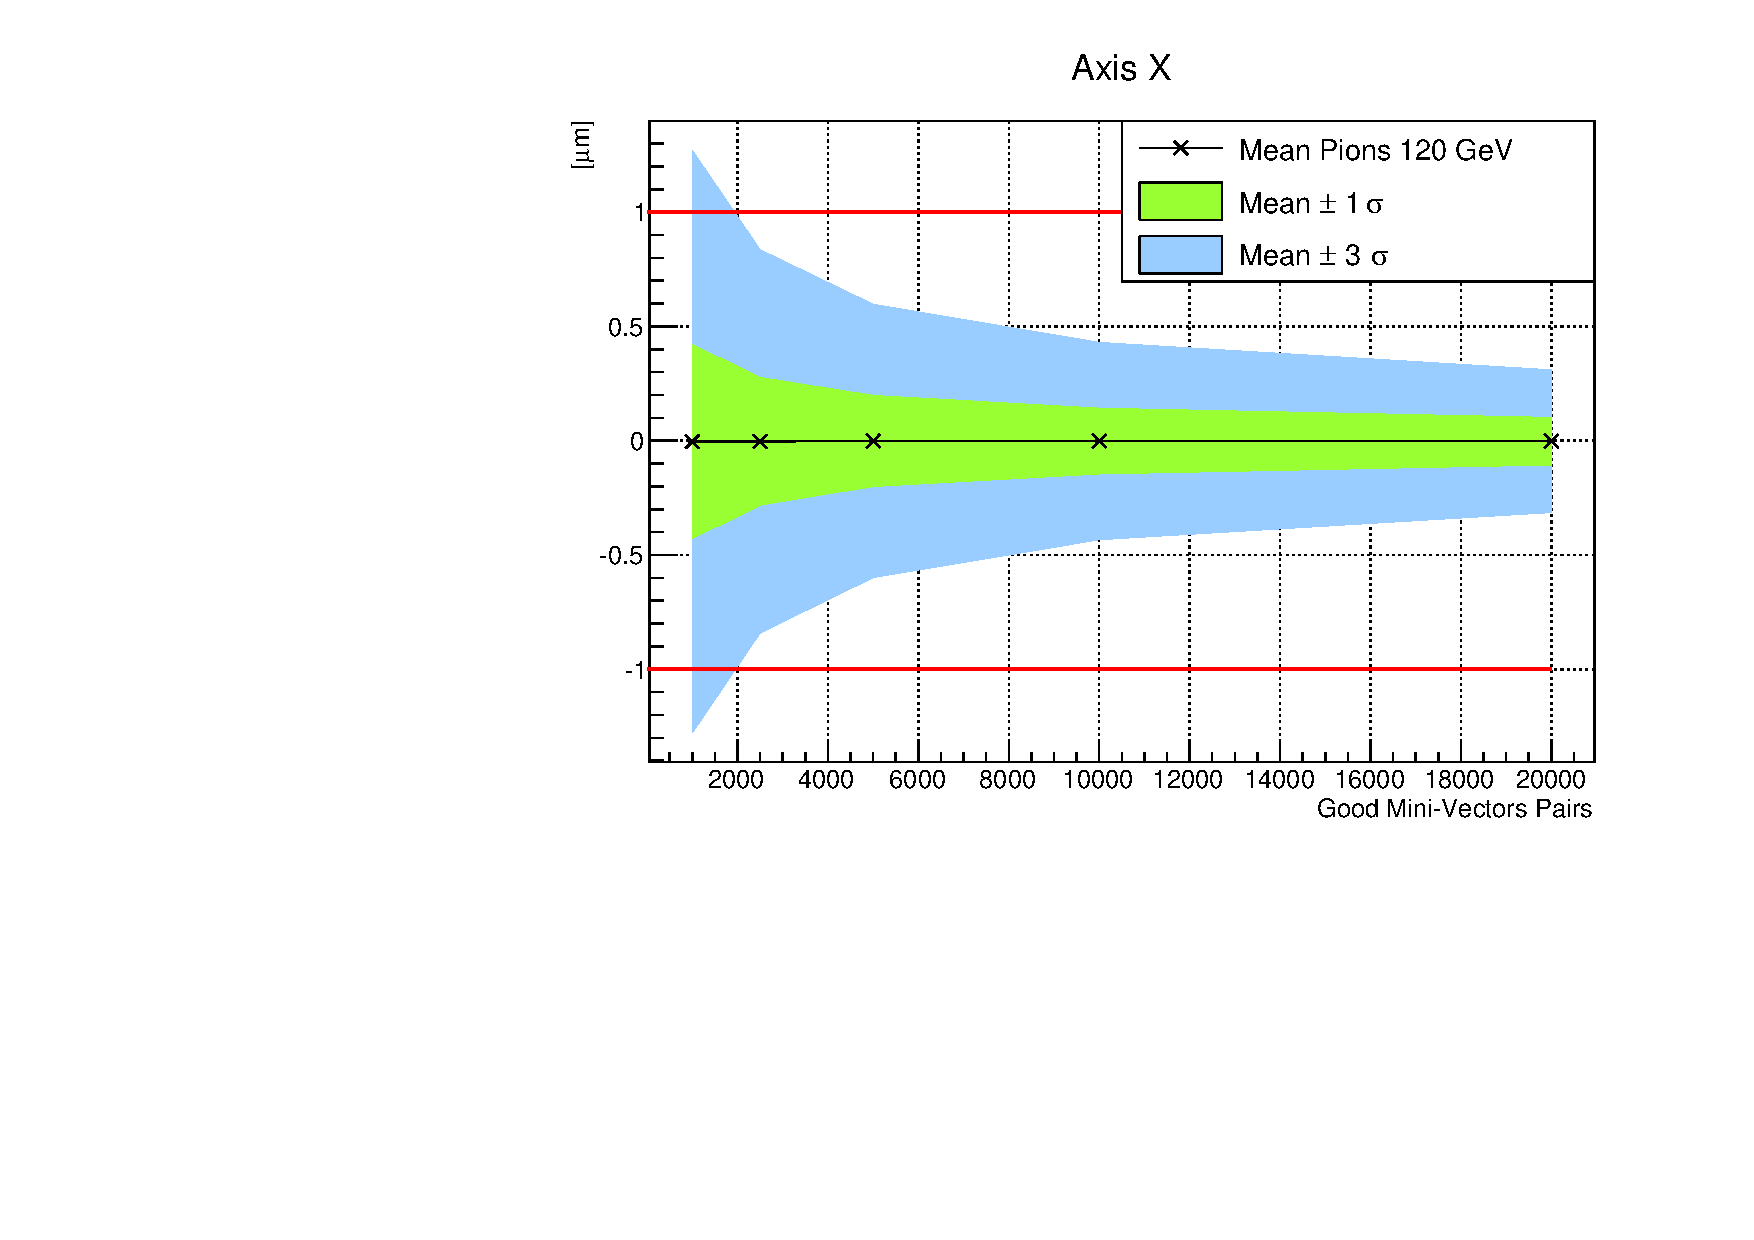
\includegraphics[width=0.82\textwidth]   {./figures/Mini_Vexteurs_Alignement_Figures/miniVectorAlignmentResults/Plots/sigmaPlots/996lines_DL3_plotSigma_Axis_X.pdf}
       }
       \subfigure[\'Ecart \`a la valeur Monte-Carlo de la valeur moyenne de la distribution du param\`etre $Y1$ apr\`es alignement, en fonction de la statistique. En vert et bleu : $\pm$ une et trois fois largeur de la distribution de ce param\`etre, en fonction de la statistique. A titre indicatif, les lignes rouges repr\'esente les valeurs de $\pm 1 \mu m$.]{
         \label{fig:MV_prec_Axe_Y_DL3}
         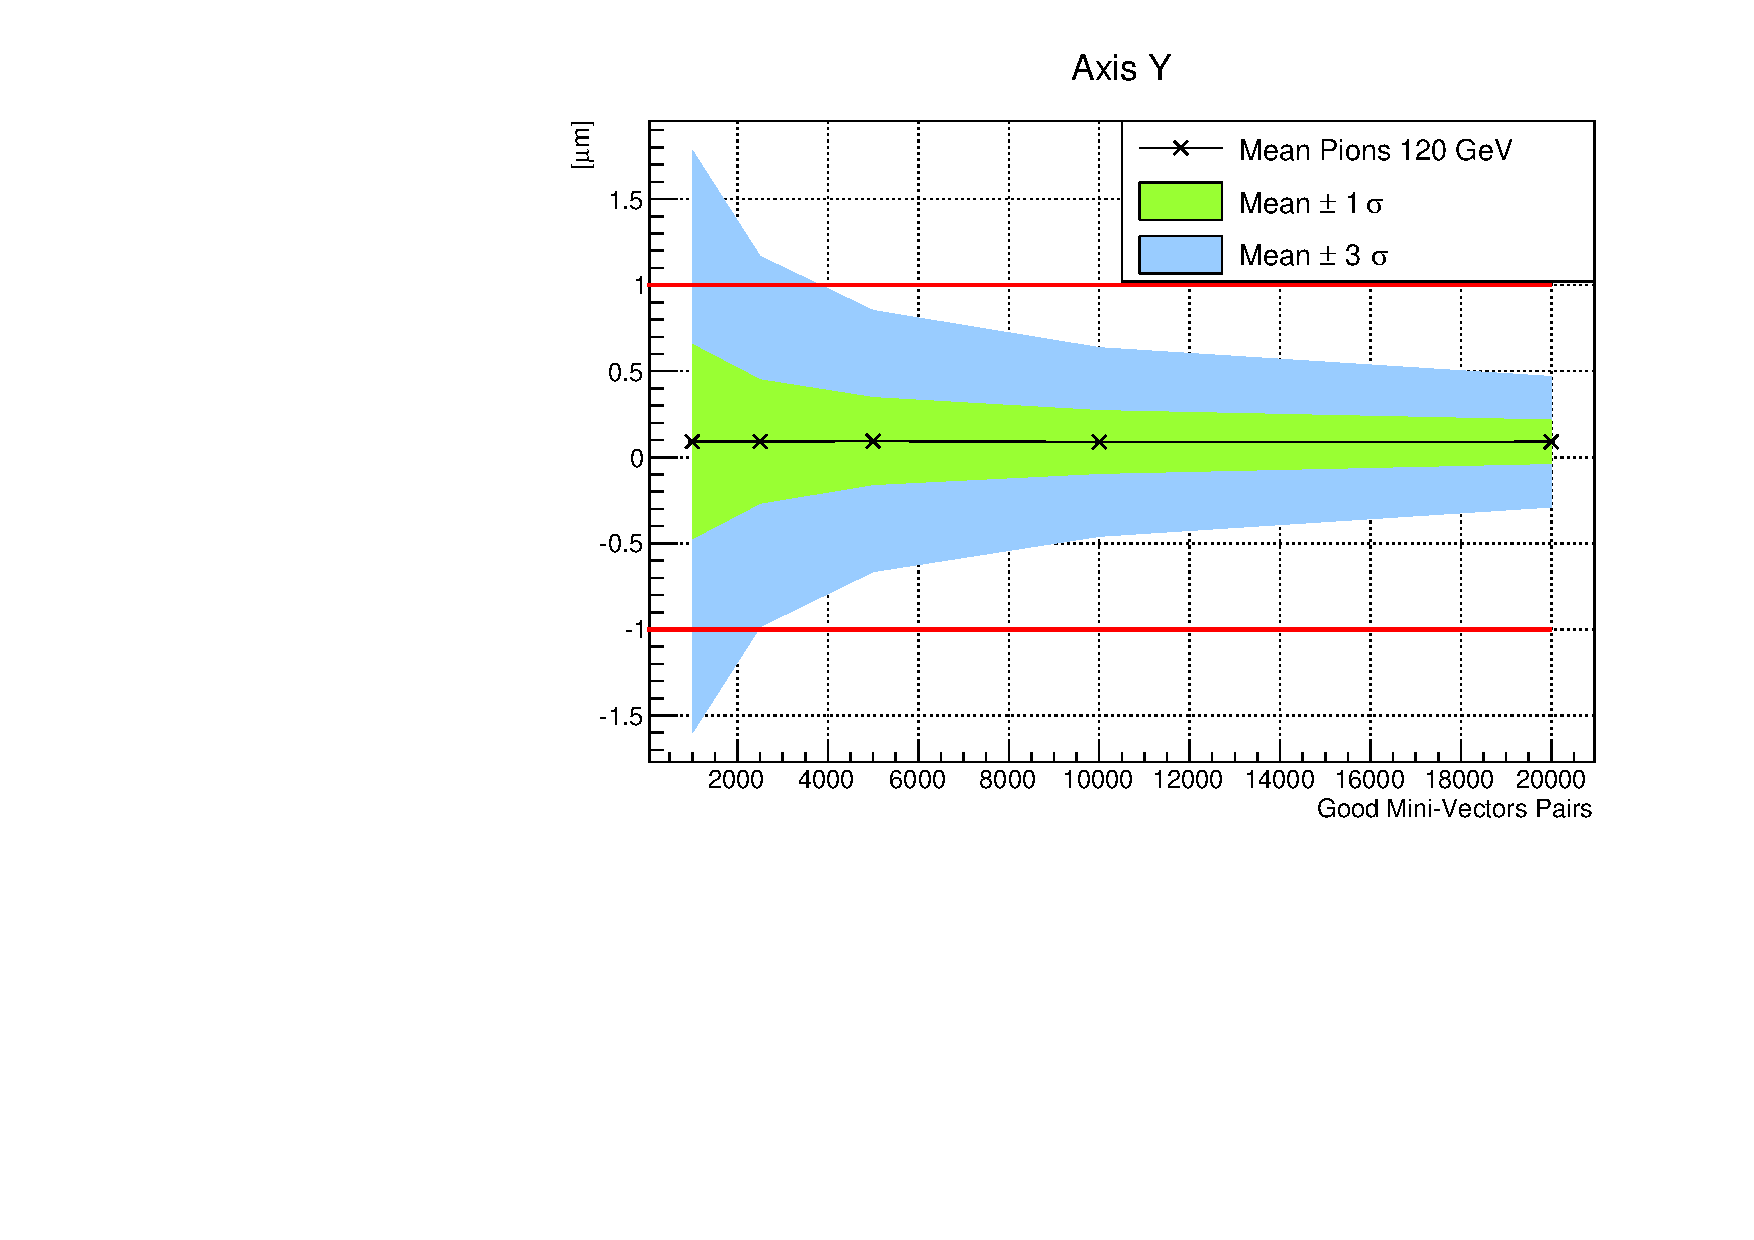
\includegraphics[width=0.82\textwidth]{./figures/Mini_Vexteurs_Alignement_Figures/miniVectorAlignmentResults/Plots/sigmaPlots/996lines_DL3_plotSigma_Axis_Y.pdf}
       }
    \end{center}
    \caption{Performances de la m\'ethode d'alignement avec mini-vecteur en fonction de la statistique utilis\'ee}
    \label{fig:Precision_0_DL3}
  \end{figure}
  
  \begin{figure}[htb!]
     \begin{center}
       \subfigure[\'Ecart \`a la valeur Monte-Carlo de la valeur moyenne de la distribution du param\`etre $Z1$ apr\`es alignement, en fonction de la statistique. En vert et bleu : $\pm$ une et trois fois largeur de la distribution de ce param\`etre, en fonction de la statistique. A titre indicatif, les lignes rouges repr\'esente les valeurs de $\pm 1 \mu m$.]{
         \label{fig:MV_prec_Axe_Z_DL3}
         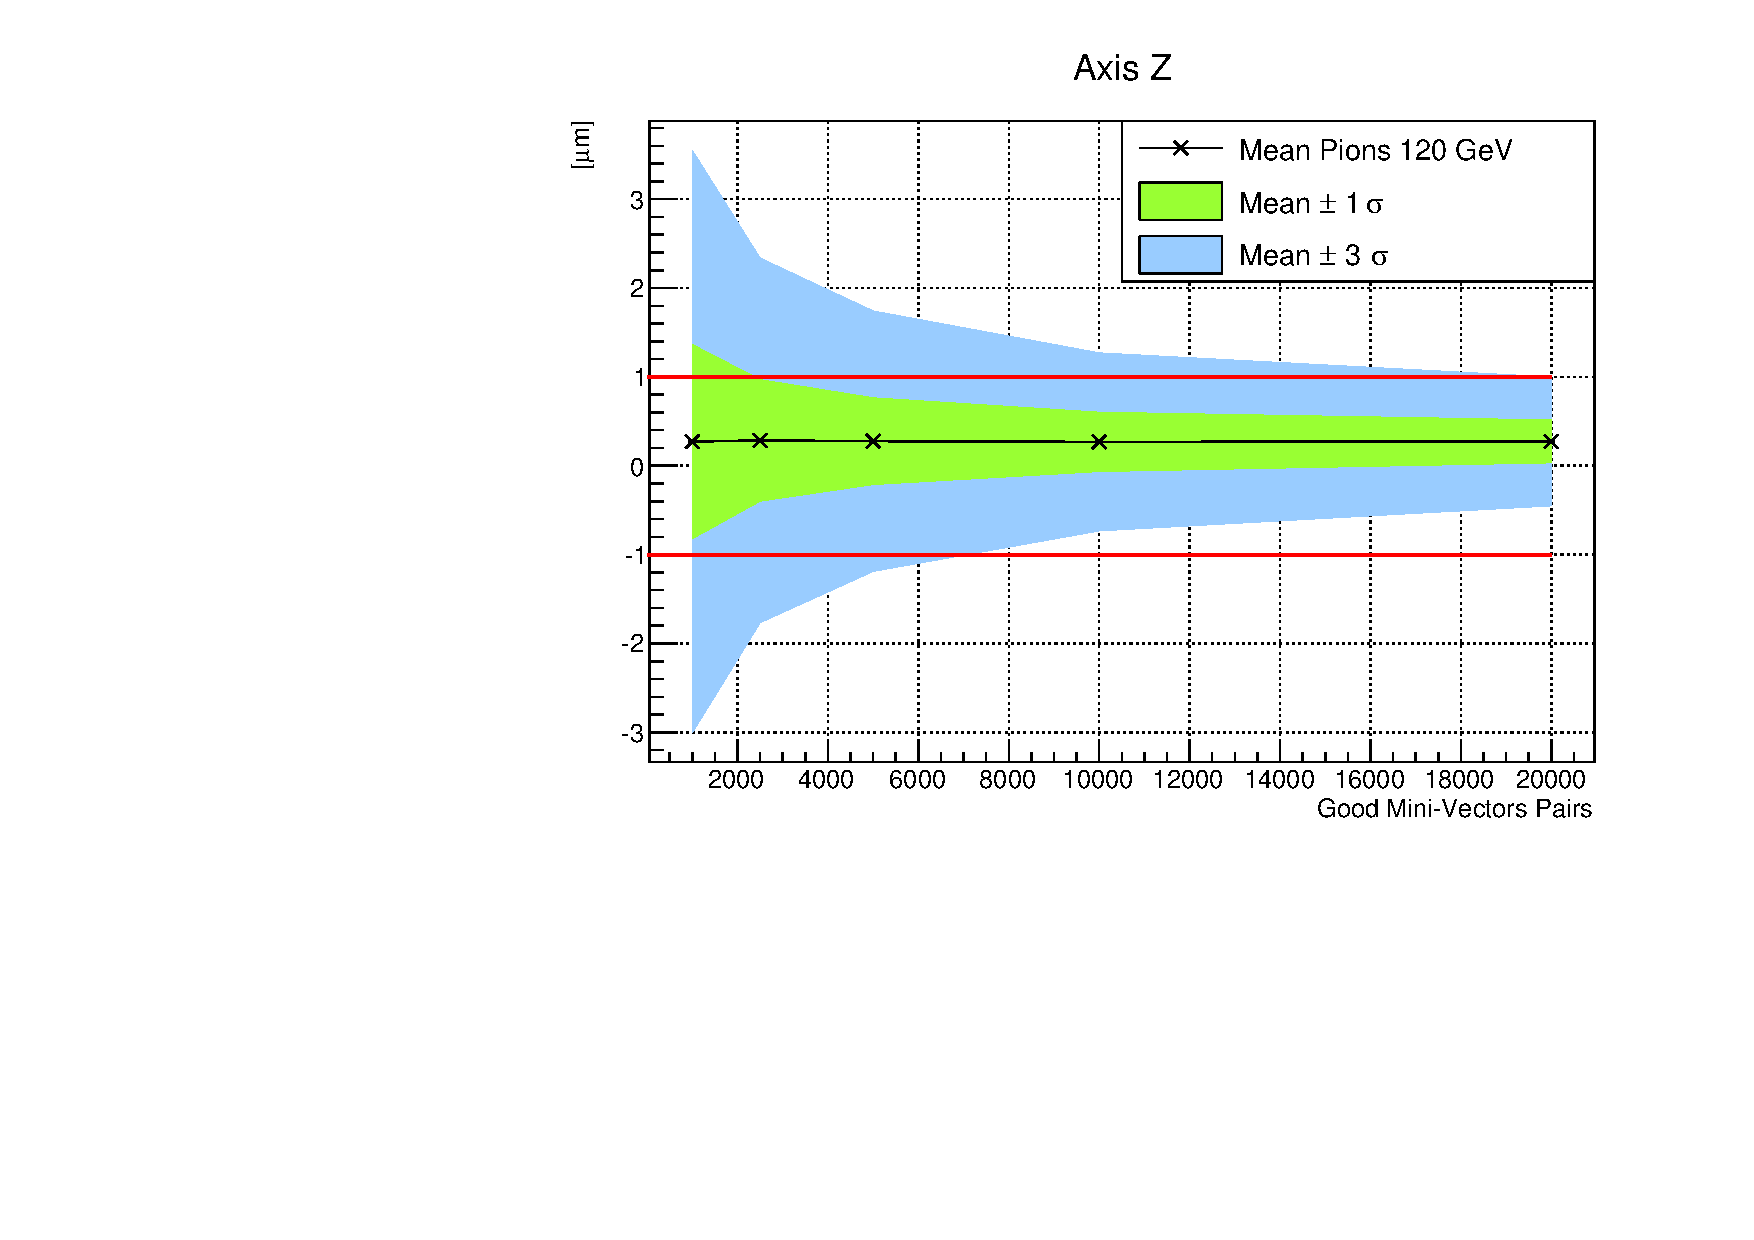
\includegraphics[width=0.78\textwidth]   {./figures/Mini_Vexteurs_Alignement_Figures/miniVectorAlignmentResults/Plots/sigmaPlots/996lines_DL3_plotSigma_Axis_Z.pdf}
       }
       \subfigure[\'Ecart \`a la valeur Monte-Carlo de la valeur moyenne de la distribution de la rotation selon l'axe $OX1$ apr\`es alignement, en fonction de la statistique. En vert et bleu : $\pm$ une et trois fois largeur de la distribution de ce param\`etre, en fonction de la statistique. A titre indicatif, les lignes rouges repr\'esente les valeurs de $\pm 1 mrad$.]{
         \label{fig:MV_prec_Rot_X_DL3}
         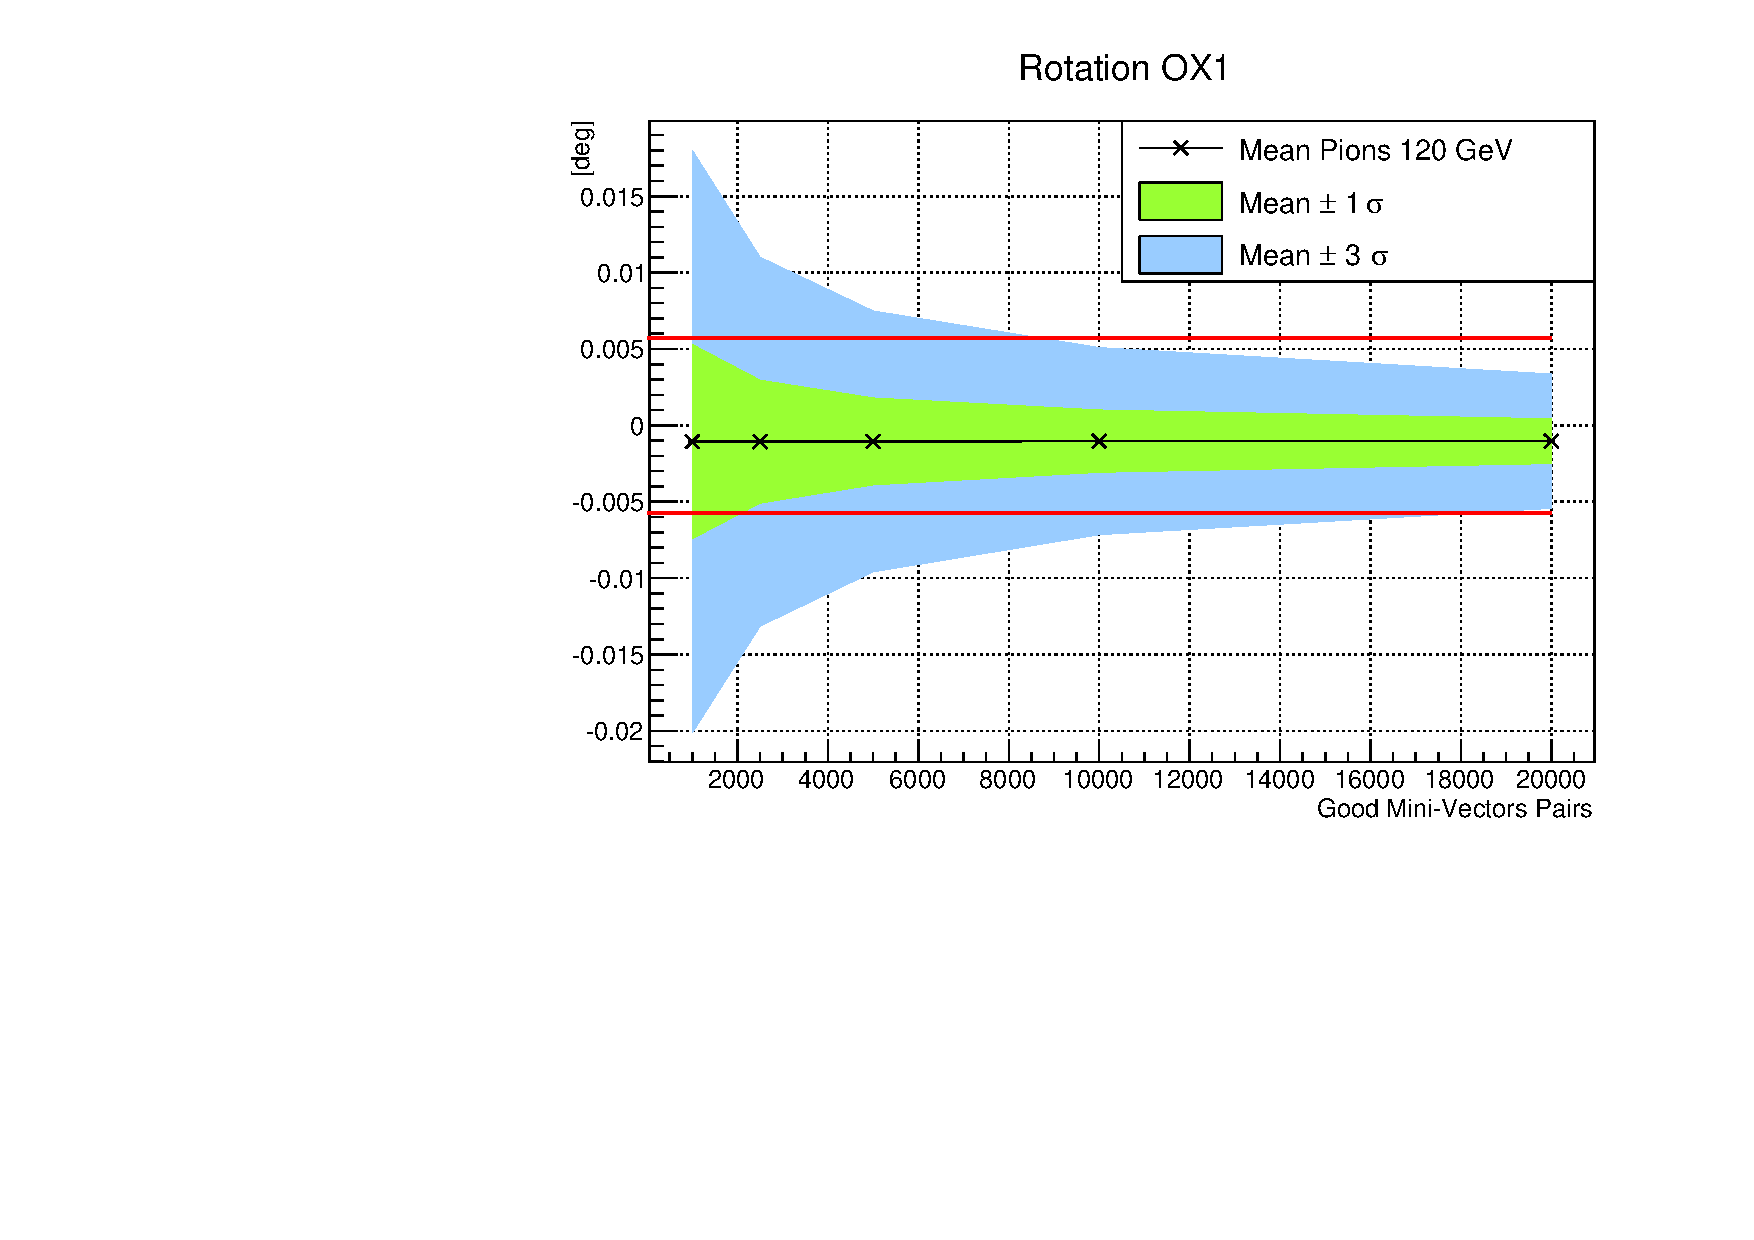
\includegraphics[width=0.78\textwidth]{./figures/Mini_Vexteurs_Alignement_Figures/miniVectorAlignmentResults/Plots/sigmaPlots/996lines_DL3_plotSigma_Rot_X.pdf}
       }
    \end{center}
    \caption{Performances de la m\'ethode d'alignement avec mini-vecteur en fonction de la statistique utilis\'ee}
    \label{fig:Precision_1_DL3}
  \end{figure}
  
  \begin{figure}[htb!]
     \begin{center}
       \subfigure[\'Ecart \`a la valeur Monte-Carlo de la valeur moyenne de la distribution de la rotation selon l'axe $OY1$ apr\`es alignement, en fonction de la statistique. En vert et bleu : $\pm$ une et trois fois largeur de la distribution de ce param\`etre, en fonction de la statistique. A titre indicatif, les lignes bleues repr\'esente les valeurs de $\pm 0.1 mrad$.]{
         \label{fig:MV_prec_Rot_Y_DL3}
         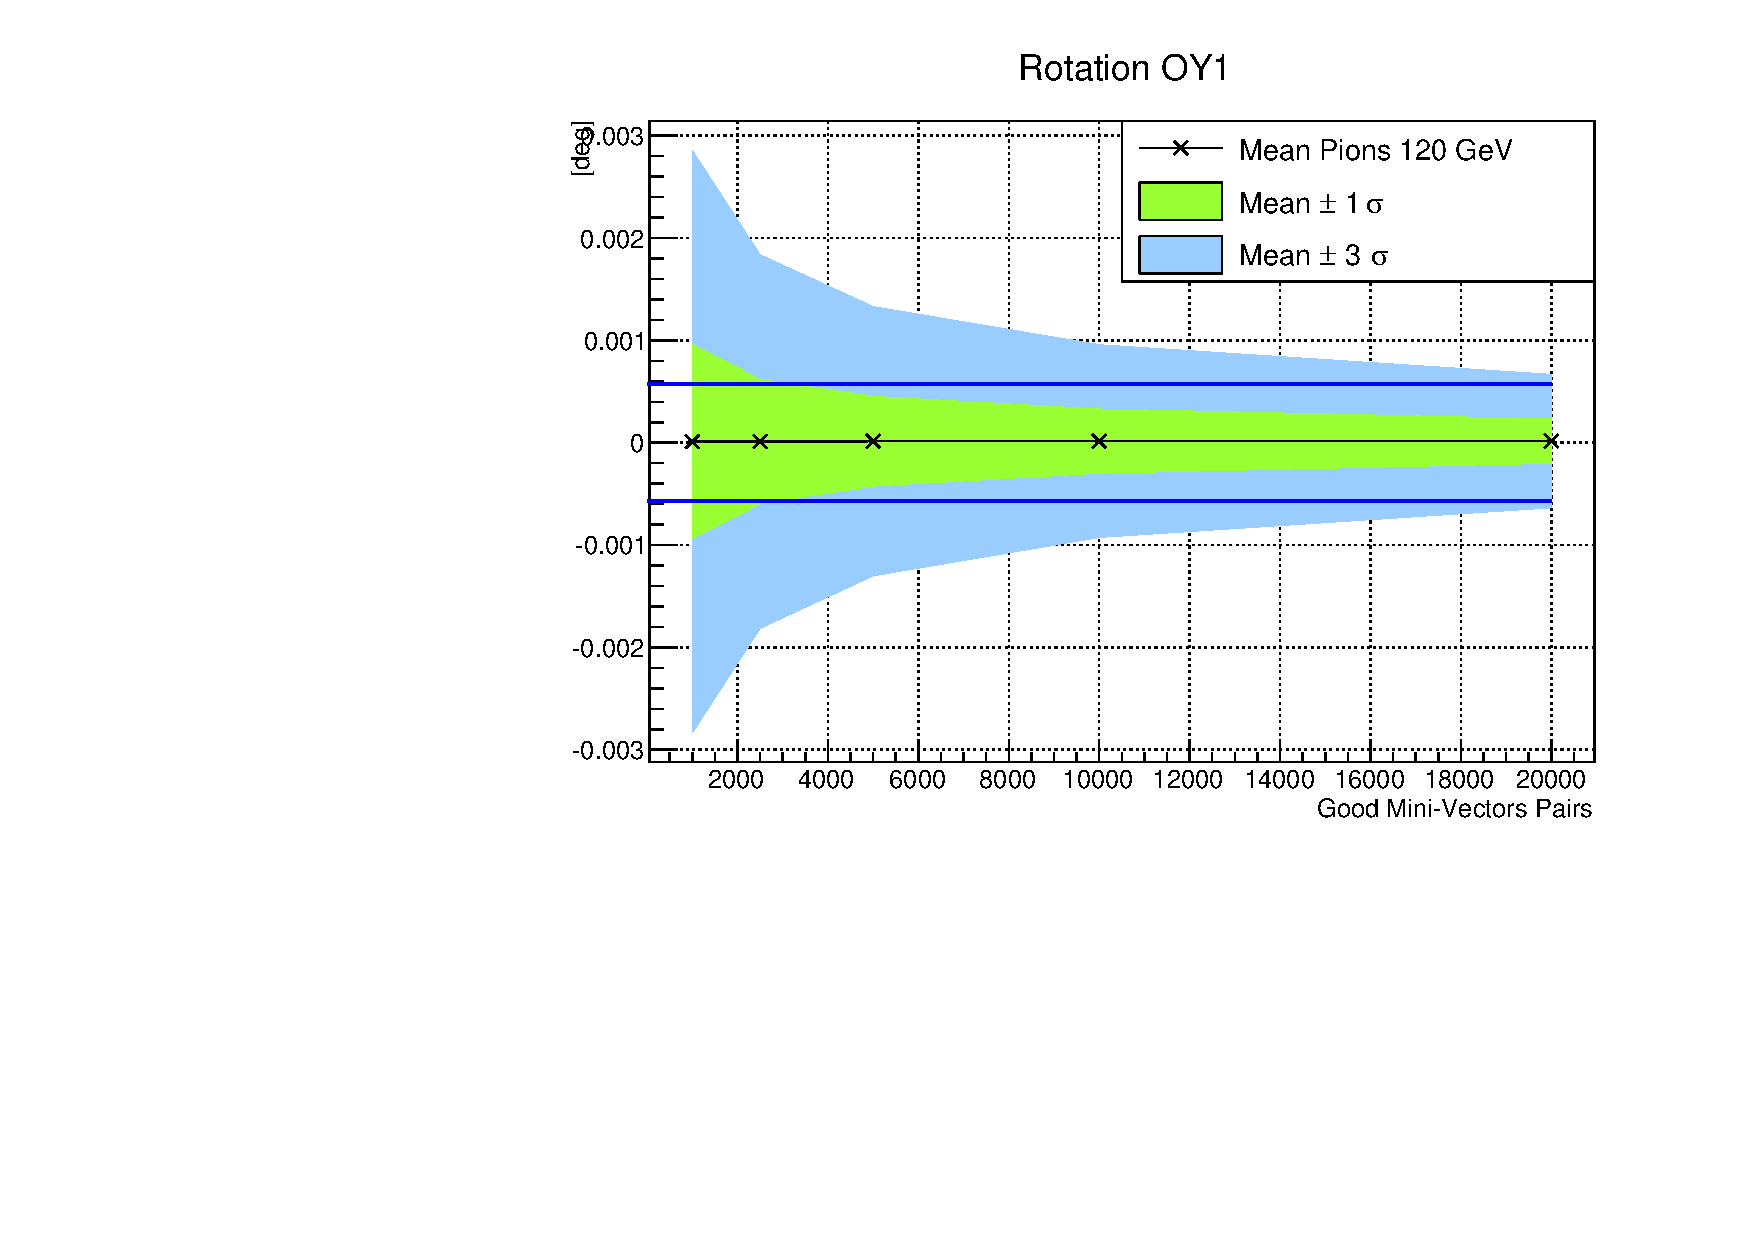
\includegraphics[width=0.78\textwidth]   {./figures/Mini_Vexteurs_Alignement_Figures/miniVectorAlignmentResults/Plots/sigmaPlots/996lines_DL3_plotSigma_Rot_Y.pdf}
       }
       \subfigure[\'Ecart \`a la valeur Monte-Carlo de la valeur moyenne de la distribution de la rotation selon l'axe $OZ1$ apr\`es alignement, en fonction de la statistique. En vert et bleu : $\pm$ une et trois fois largeur de la distribution de ce param\`etre, en fonction de la statistique. A titre indicatif, les lignes bleues repr\'esente les valeurs de $\pm 0.1 mrad$]{
         \label{fig:MV_prec_Rot_Z_DL3}
         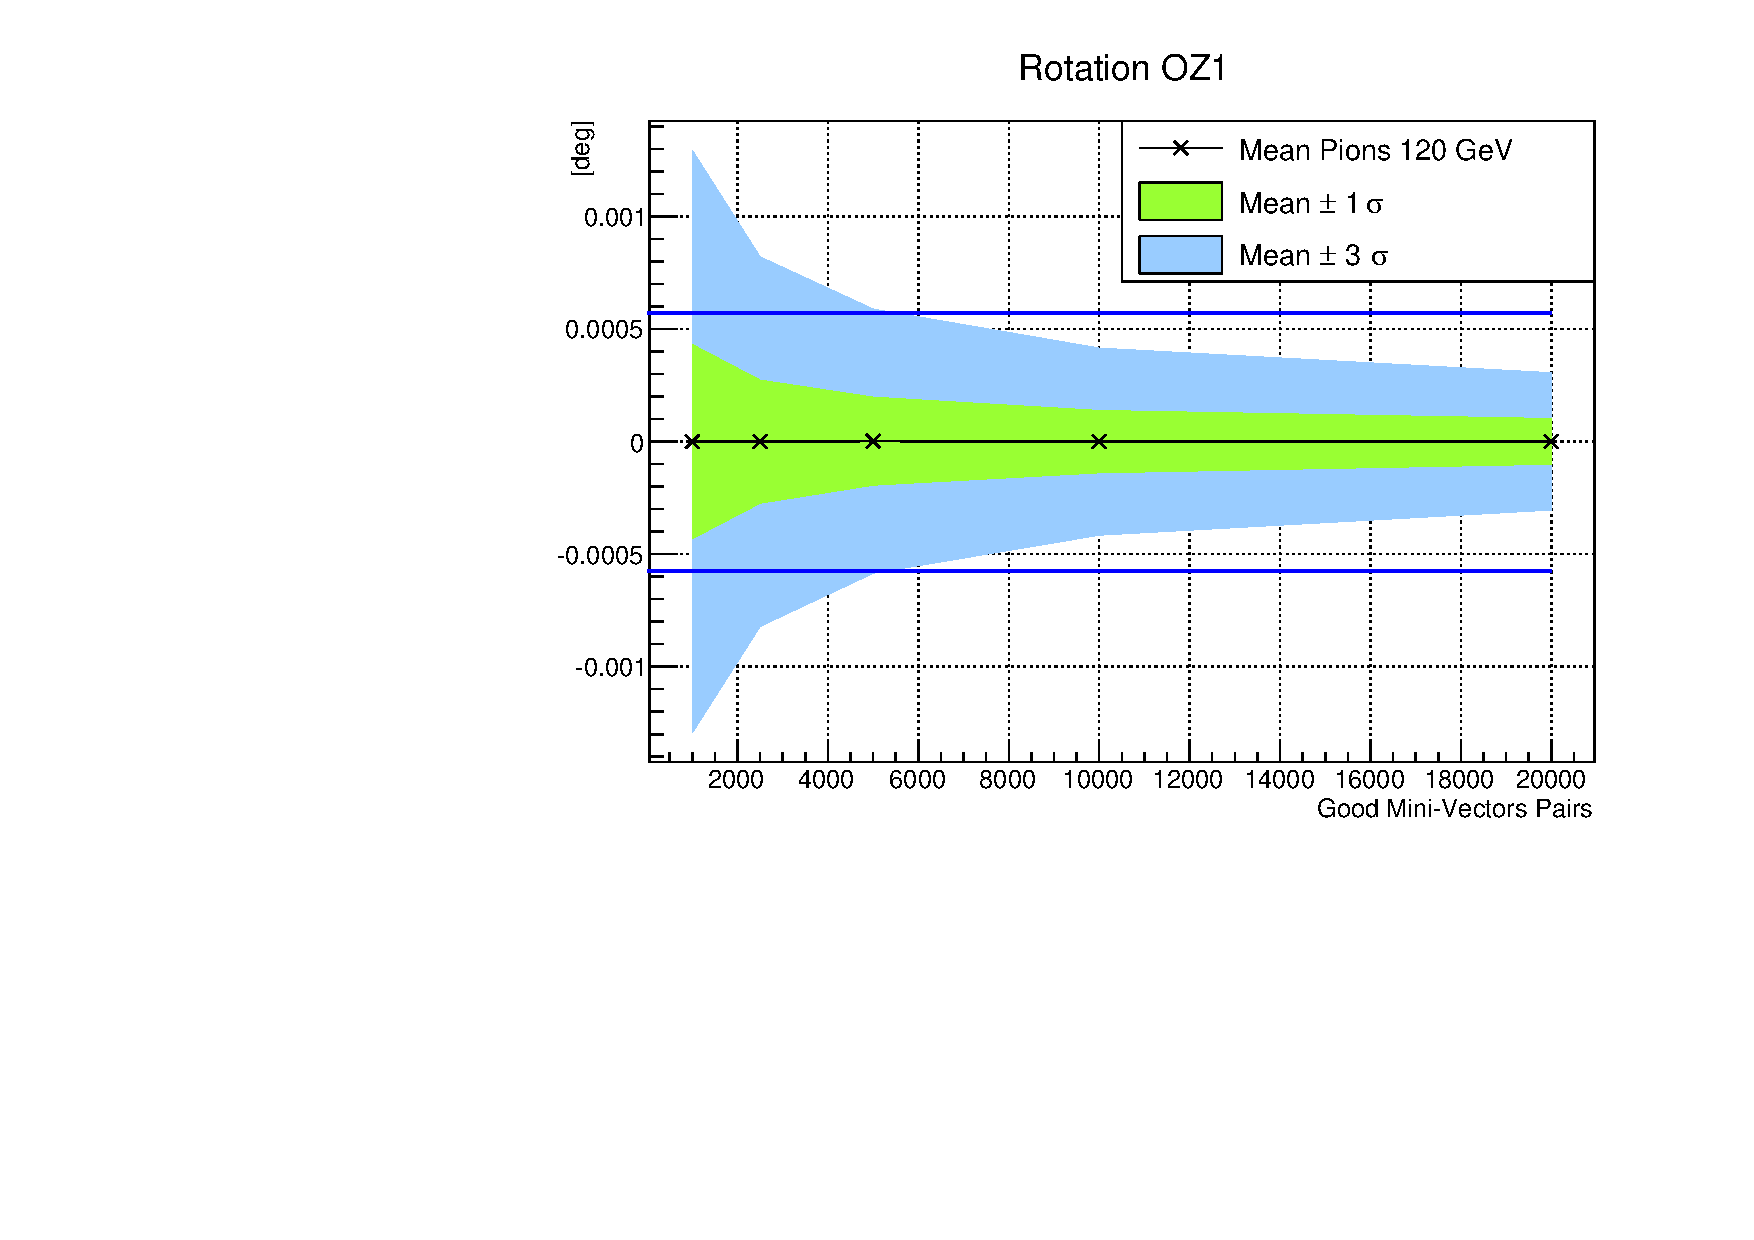
\includegraphics[width=0.78\textwidth]{./figures/Mini_Vexteurs_Alignement_Figures/miniVectorAlignmentResults/Plots/sigmaPlots/996lines_DL3_plotSigma_Rot_Z.pdf}
       }
    \end{center}
    \caption{Performances de la m\'ethode d'alignement avec mini-vecteur en fonction de la statistique utilis\'ee}
    \label{fig:Precision_2_DL3}
  \end{figure}
% 
% \chapter{D\'esalignement de 500 microns sur l'axe O1X} 
% \label{annexe}
% 
%   L'objectif de  de cette section est de caract\'eriser la m\'ethode d'alignement avec mini-vecteurs. Pour cela, la dispersion et les valeurs des param\`etres de l'\'echelle \`a aligner (position de son centre et ses 3 inclinaisons) apr\`es alignement ont \'et\'e \'etudi\'ees. 
%   
%    \medskip
%    Un d\'esalignemnt de +500 $\mu m$ selon l'axe $O1X$ a \'et\'e utilis\'e. Plusieurs lots de donn\'ees contenant un nombre N de couples de mini-vecteurs après coupures, ont \'et\'e minimis\'es. Chacun de ces lots est r\'ealis\'e avec des donn\'ees diff\'erentes. Environ 4 500 000 millions \'ev\'enements, passant par la zone de recouvrement des deux \'echelles ont \'et\'e utilis\'es. Les coupures $\Delta Res = 800 \mu m$ et $\Delta Pente = 10$ ont \'et\'e appliqu\'ees.
%    
% %   \medskip
%   
% %  La figure \ref{fig:MV_After_Mini_Tr_X} expose la distribution de la coordonn\'ee $X1$ du centre de l'\'echelle apr\`es alignements. Pour cela, 4284 lots de donn\'ees diff\'erents, comportant chacun 1000 couples de mini-vecteurs, ont \'et\'e minimis\'es. 
%   
%    \begin{figure}[htb!]
%      \begin{center}
%         \subfigure[Distribution de la coordonn\'ee $X1$ du centre de l'\'echelle apr\`es alignements. 4284 lots de donn\'ees diff\'erents ont \'et\'e minimis\'es. Chacun de ces lots comporte 1000 couples de mini-vecteurs. La valeur attendue 0 est retrouv\'ee.]{
%             \label{fig:MV_After_Mini_Tr_X_500mum}
%             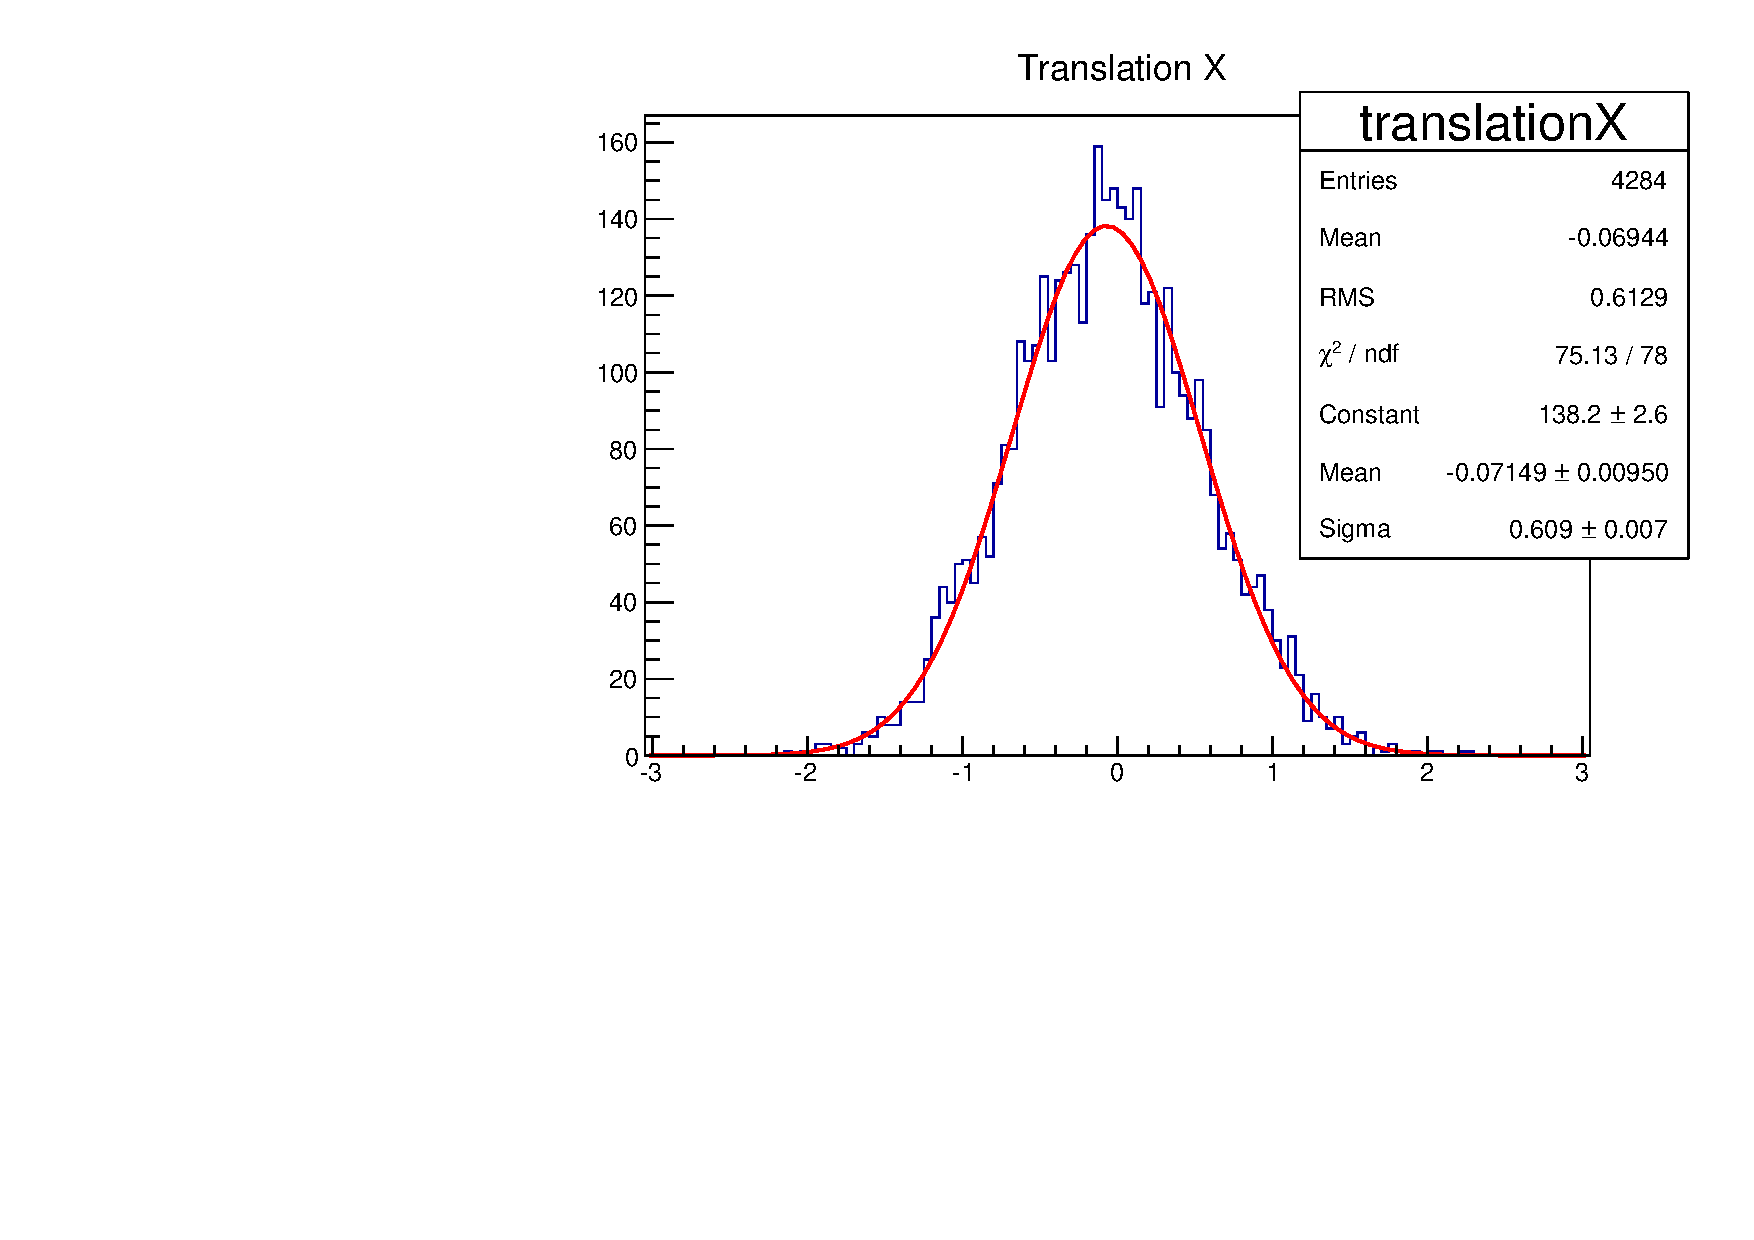
\includegraphics[width=0.82\textwidth]{./figures/Mini_Vexteurs_Alignement_Figures/After_Mini_Tr_X_1000_Tracks.pdf}
%         }
%         \subfigure[Distribution de la coordonn\'ee $Y1$ du centre de l'\'echelle apr\`es alignements. 4284 lots de donn\'ees diff\'erents ont \'et\'e minimis\'es. Chacun de ces lots comporte 1000 couples de mini-vecteurs. La valeur attendue 7500 est retrouv\'ee.]{
%            \label{fig:MV_After_Mini_Tr_Y_500mum}
%            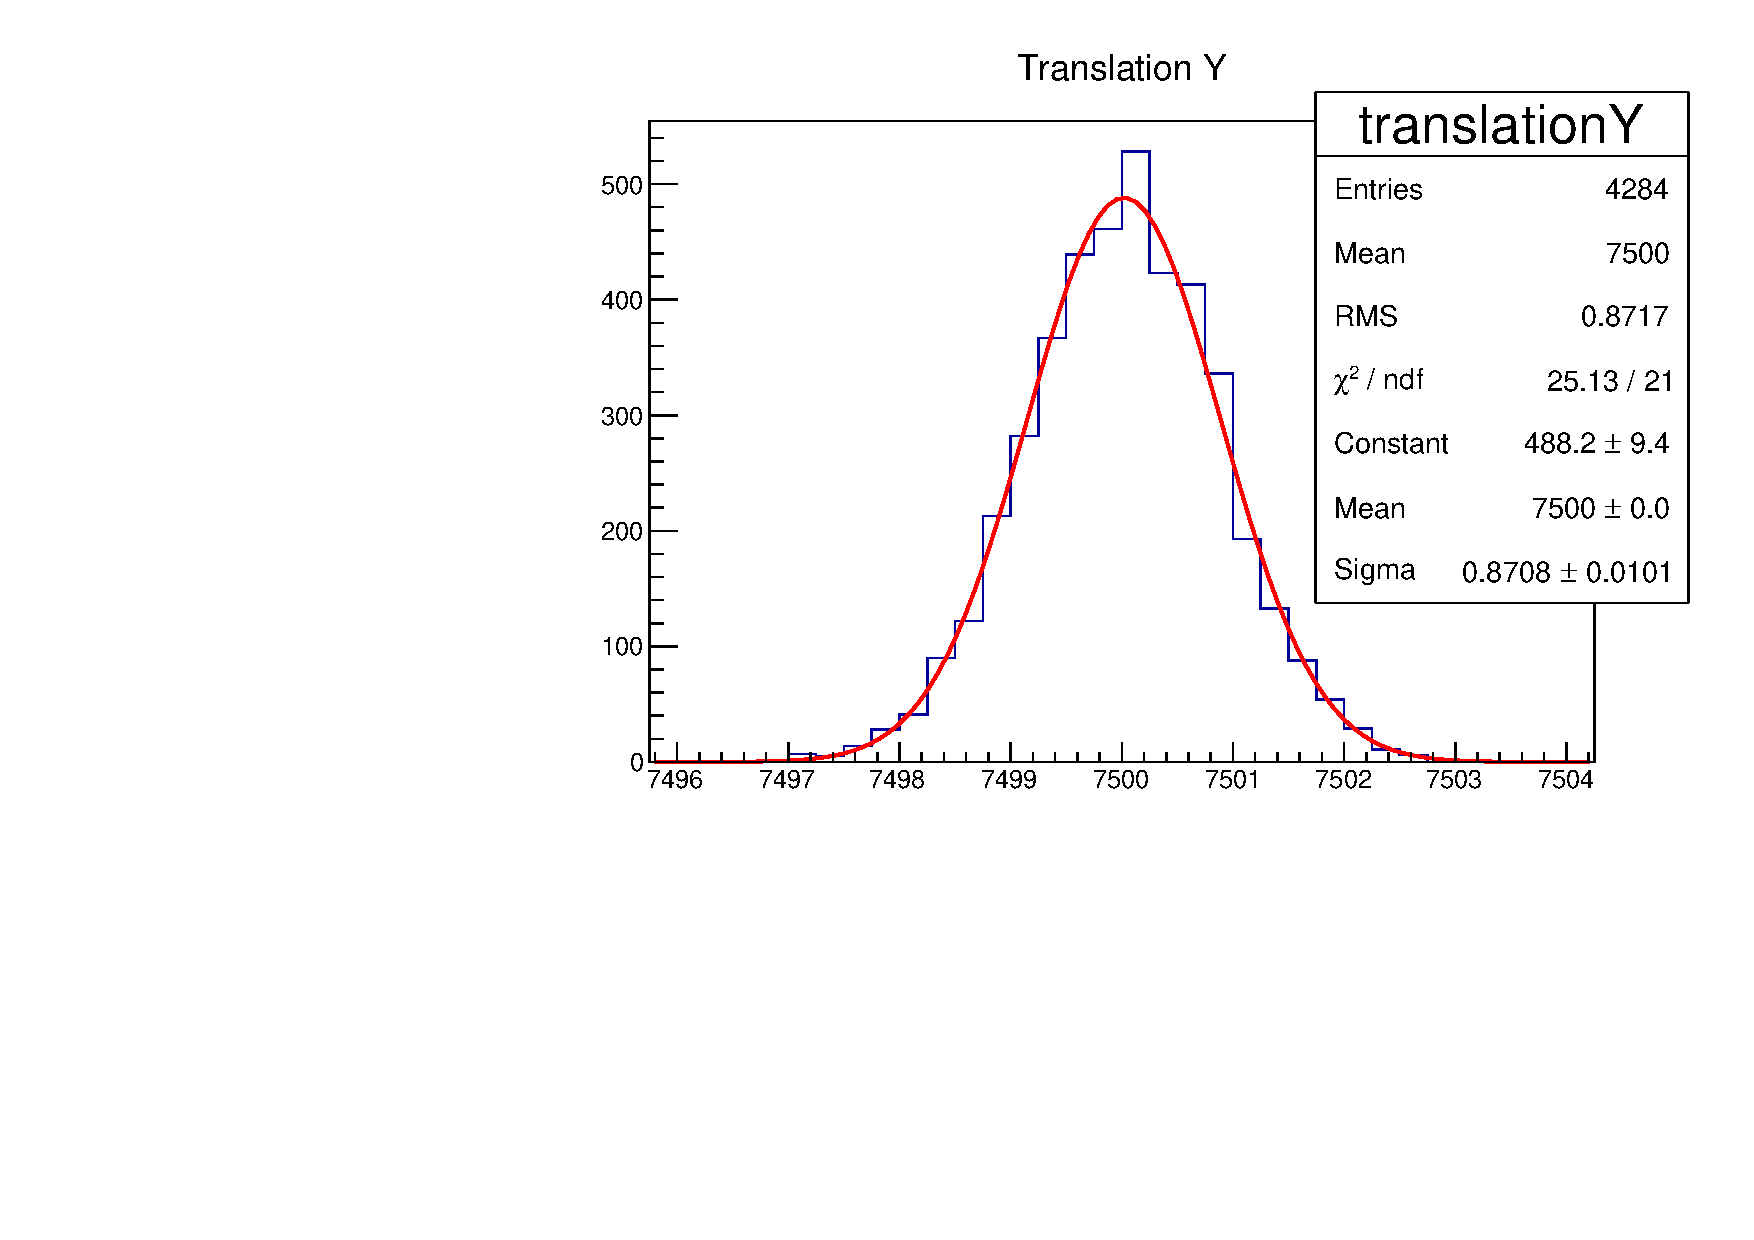
\includegraphics[width=0.82\textwidth]{./figures/Mini_Vexteurs_Alignement_Figures/After_Mini_Tr_Y_1000_Tracks.pdf}
%         }
%      \end{center}
%      \caption{Distributions de param\`etres de l'\'echelle 1 apr\`es alignement}
%      \label{fig:0_500mum}
%    \end{figure}
%   
%   \FloatBarrier
%   
% %   La distribution obtenue est alors ajust\'ee avec une fonction Gaussienne. Cette derni\`ere est centr\'ee sur la valeur $-0.07 \, \mu m$ et poss\`ede une largeur d'environ $0.61 \, \mu m$. La valeur $X1 = 0$ est bien retrouv\'ee.
% %   
% %   \medskip
% % 
% %   La figure \ref{fig:MV_After_Mini_Tr_Y} montre la distribution de la coordonn\'ee $Y1$ du centre de l'\'echelle apr\`es alignements. Pour cela, 4284 lots de donn\'ees diff\'erents, comportant chacun 1000 couples de mini-vecteurs, ont \'et\'e minimis\'es. La distribution obtenue est alors ajust\'ee avec une fonction Gaussienne. Cette derni\`ere est centr\'ee sur la valeur $7500 \, \mu m$ et poss\`ede une largeur d'environ $0.87 \mu m$. La valeur $Y1 = 7 500$ est bien retrouv\'ee.  
% % 
% %   \medskip
% % 
% %   La figure \ref{fig:MV_After_Mini_Tr_Z} donne la distribution de la coordonn\'ee $Z1$ du centre de l'\'echelle apr\`es alignements. Pour cela, 4284 lots de donn\'ees diff\'erents, comportant chacun 1000 couples de mini-vecteurs, ont \'et\'e minimis\'es. La distribution obtenue est alors ajust\'ee avec une fonction Gaussienne. Cette derni\`ere est centr\'ee sur la valeur $34 990 \, \mu m$ et poss\`ede une largeur d'environ $6.30 \mu m$. La valeur $Z1 = 35 000$ n'est cette fois-ci pas retrouv\'ee pr\'ecis\'ement. Un d\'ecalage d'environ $-10 \, \mu m$ est observ\'e.
% %   
% %   \medskip
%   
%    \begin{figure}[htb!]
%      \begin{center}
%         \subfigure[Distribution de la coordonn\'ee $Z1$ du centre de l'\'echelle 1 apr\`es alignements. 4284 lots de donn\'ees diff\'erents ont \'et\'e minimis\'es. Chacun de ces lots comporte 1000 couples de mini-vecteurs. La valeur attendue vaut 35000. Un \'ecart de 10 $\mu m$ est observ\'e.]{
%             \label{fig:MV_After_Mini_Tr_Z_500mum}
%             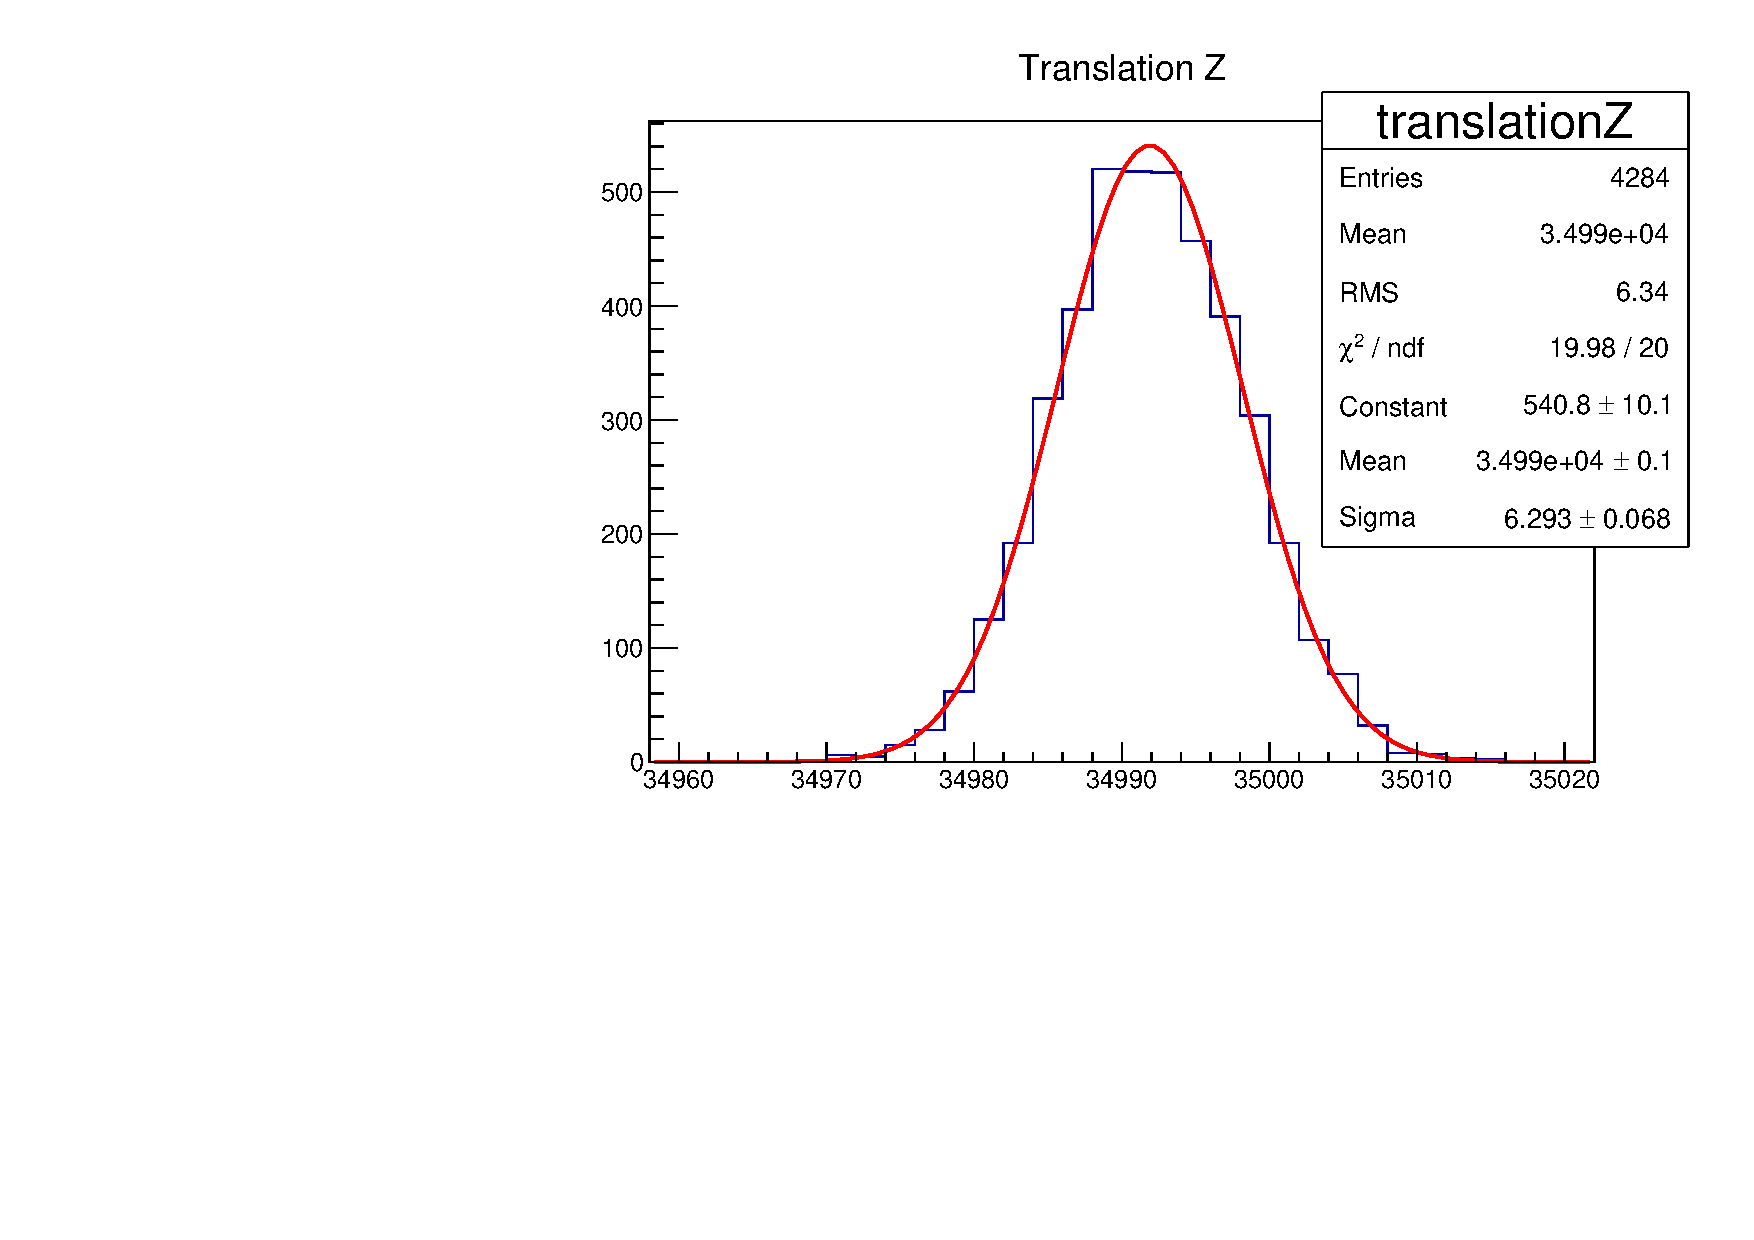
\includegraphics[width=0.80\textwidth]{./figures/Mini_Vexteurs_Alignement_Figures/After_Mini_Tr_Z_1000_Tracks.pdf}
%         }
%         \subfigure[Distribution de l'inclinaison de l'\'echelle 1 selon son axe $C1X$, apr\`es alignements. 4284 lots de donn\'ees diff\'erents ont \'et\'e minimis\'es. Chacun de ces lots comporte 1000 couples de mini-vecteurs. La valeur entendu de 30 degr\'es est retrouv\'ee]{
%            \label{fig:MV_After_Mini_Rot_X_500mum}
%            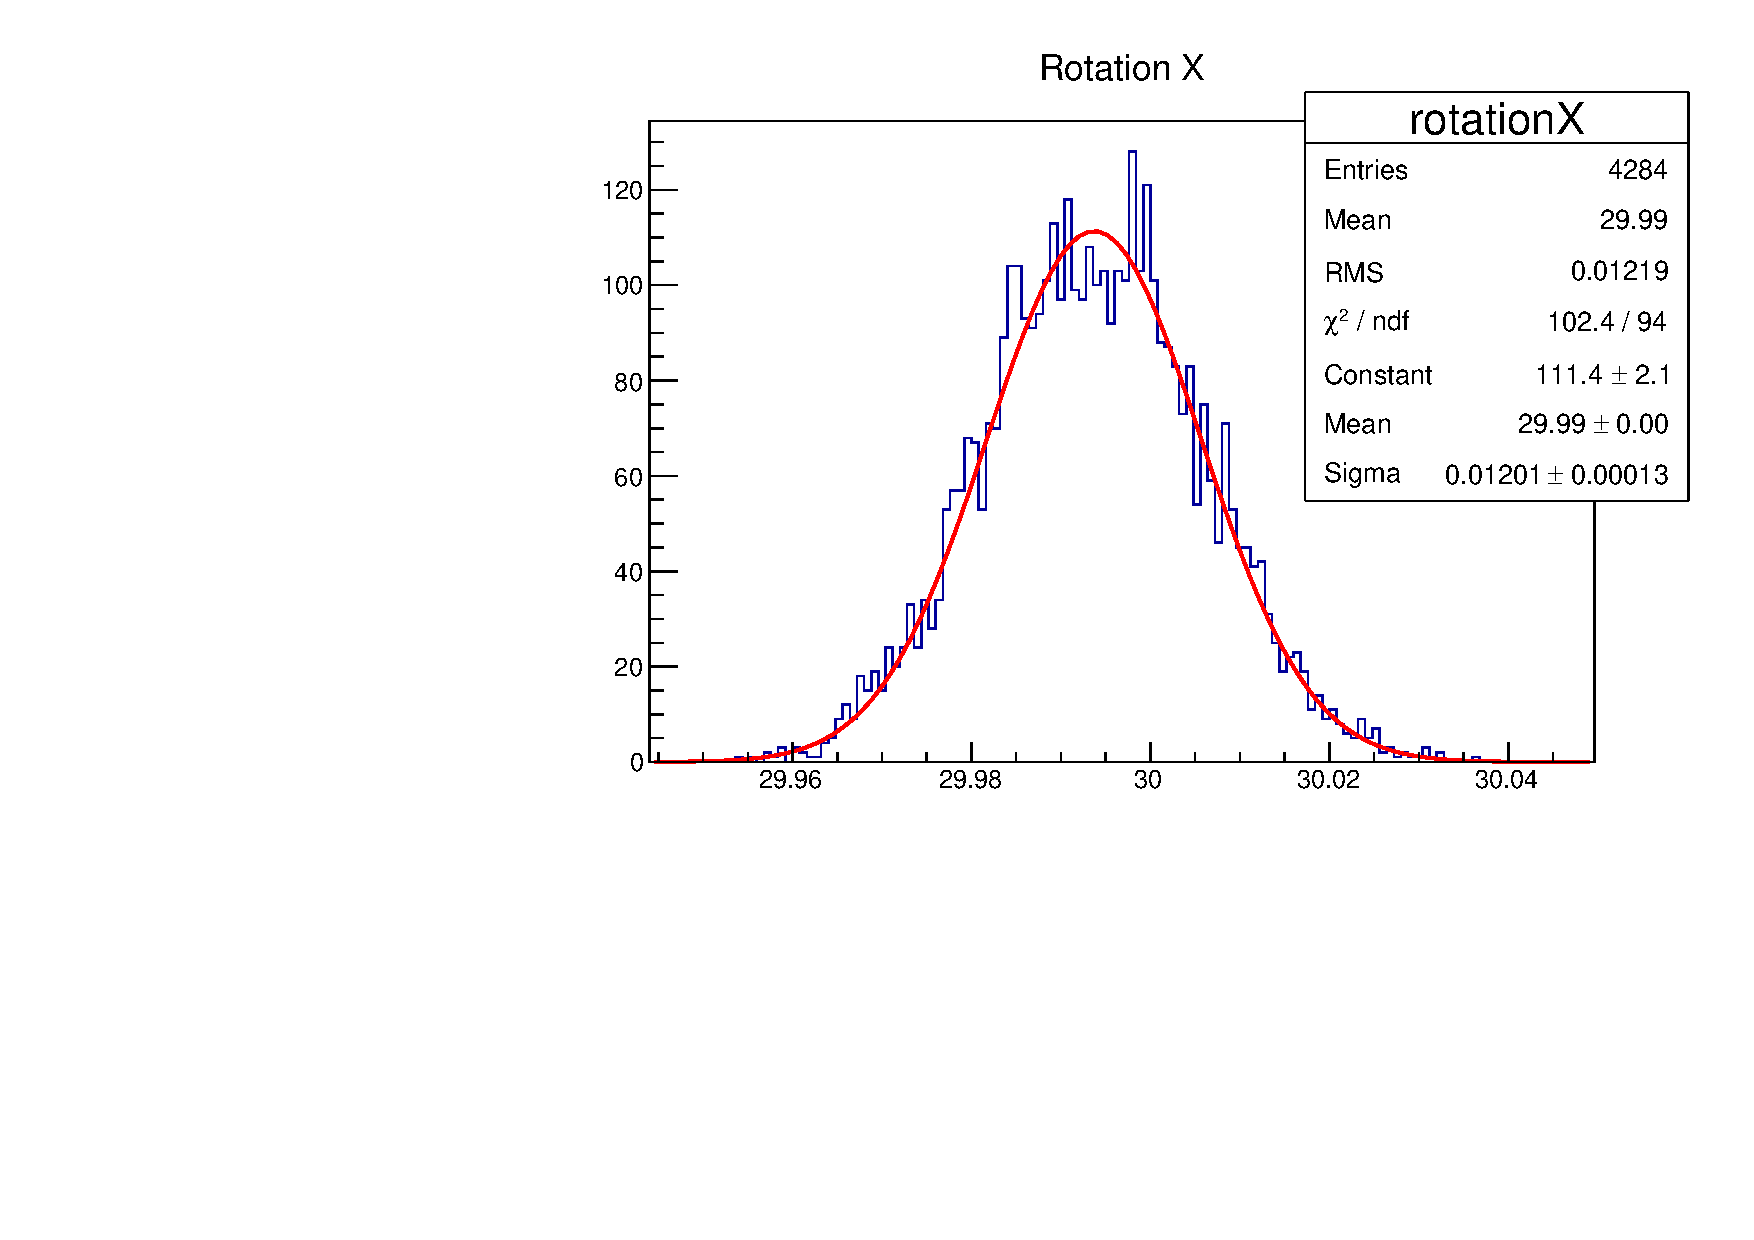
\includegraphics[width=0.80\textwidth]{./figures/Mini_Vexteurs_Alignement_Figures/After_Mini_Rot_X_1000_Tracks.pdf}
%         }
%      \end{center}
%      \caption{Distributions de param\`etres de l'\'echelle 1 apr\`es alignement}
%      \label{fig:1_500mum}
%    \end{figure}
%   
% %   La figure \ref{fig:MV_After_Mini_Rot_X} repr\'esente la distribution de l'inclinaison $angleX$ de l'\'echelle apr\`es alignements. Pour cela, 4284 lots de donn\'ees diff\'erents, comportant chacun 1000 couples de mini-vecteurs, ont \'et\'e minimis\'es. La distribution obtenue est alors ajust\'ee avec une fonction Gaussienne. Cette derni\`ere est centr\'ee sur la valeur $29.99$ degr\'es et poss\`ede une largeur d'environ $0.01$ degr\'e. La valeur $angleX = 30$ degr\'es est bien retrouv\'ee.  
% %   
% %   \medskip
% %   
% %   La figure \ref{fig:MV_After_Mini_Rot_Y} repr\'esente la distribution de l'inclinaison $angleY$ de l'\'echelle apr\`es alignements. Pour cela, 4284 lots de donn\'ees diff\'erents, comportant chacun 1000 couples de mini-vecteurs, ont \'et\'e minimis\'es. La distribution obtenue est alors ajust\'ee avec une fonction Gaussienne. Cette derni\`ere est centr\'ee sur la valeur $1.8 \, 10^{-4}$ degr\'e et poss\`ede une largeur d'environ $8 \, 10^{-3}$ degr\'e. La valeur $angleY = 0$ degr\'es est bien retrouv\'ee.
% %   
% %   \medskip
% 
%     \begin{figure}[htb!]
%      \begin{center}
%         \subfigure[Distribution de l'inclinaison de l'\'echelle 1 selon son axe $C1Y$ apr\`es alignements. 4284 lots de donn\'ees diff\'erents ont \'et\'e minimis\'es. Chacun de ces lots comporte 1000 couples de mini-vecteurs. La valeur entendu  de 0 degr\'es est retrouv\'ee]{
%             \label{fig:MV_After_Mini_Rot_Y_500mum}
%             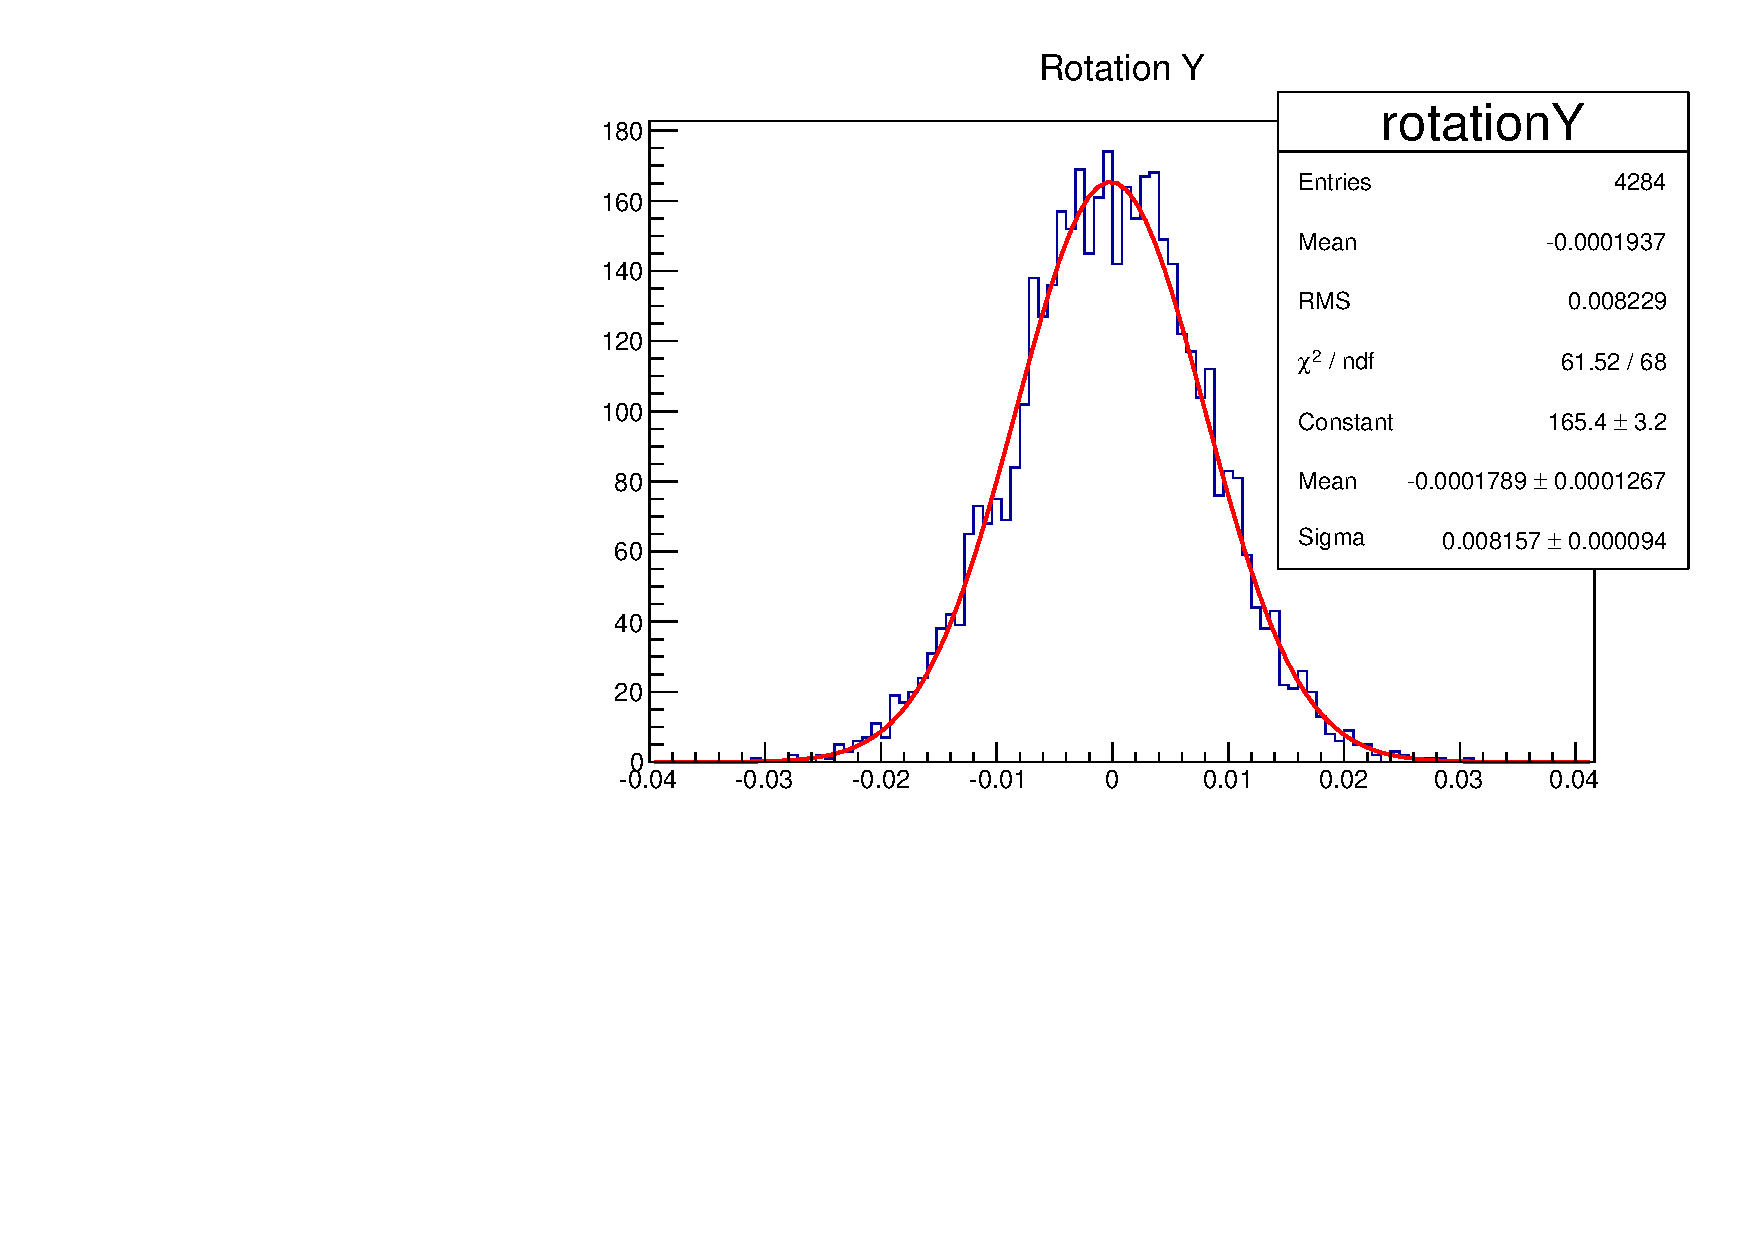
\includegraphics[width=0.80\textwidth]{./figures/Mini_Vexteurs_Alignement_Figures/After_Mini_Rot_Y_1000_Tracks.pdf}
%         }
%         \subfigure[Distribution de l'inclinaison de l'\'echelle 1 selon son axe $C1Z$ apr\`es alignements. 4284 lots de donn\'ees diff\'erents ont \'et\'e minimis\'es. Chacun de ces lots comporte 1000 couples de mini-vecteurs. La valeur entendu de 0 degr\'es est retrouv\'ee]{
%            \label{fig:MV_After_Mini_Rot_Z_500mum}
%            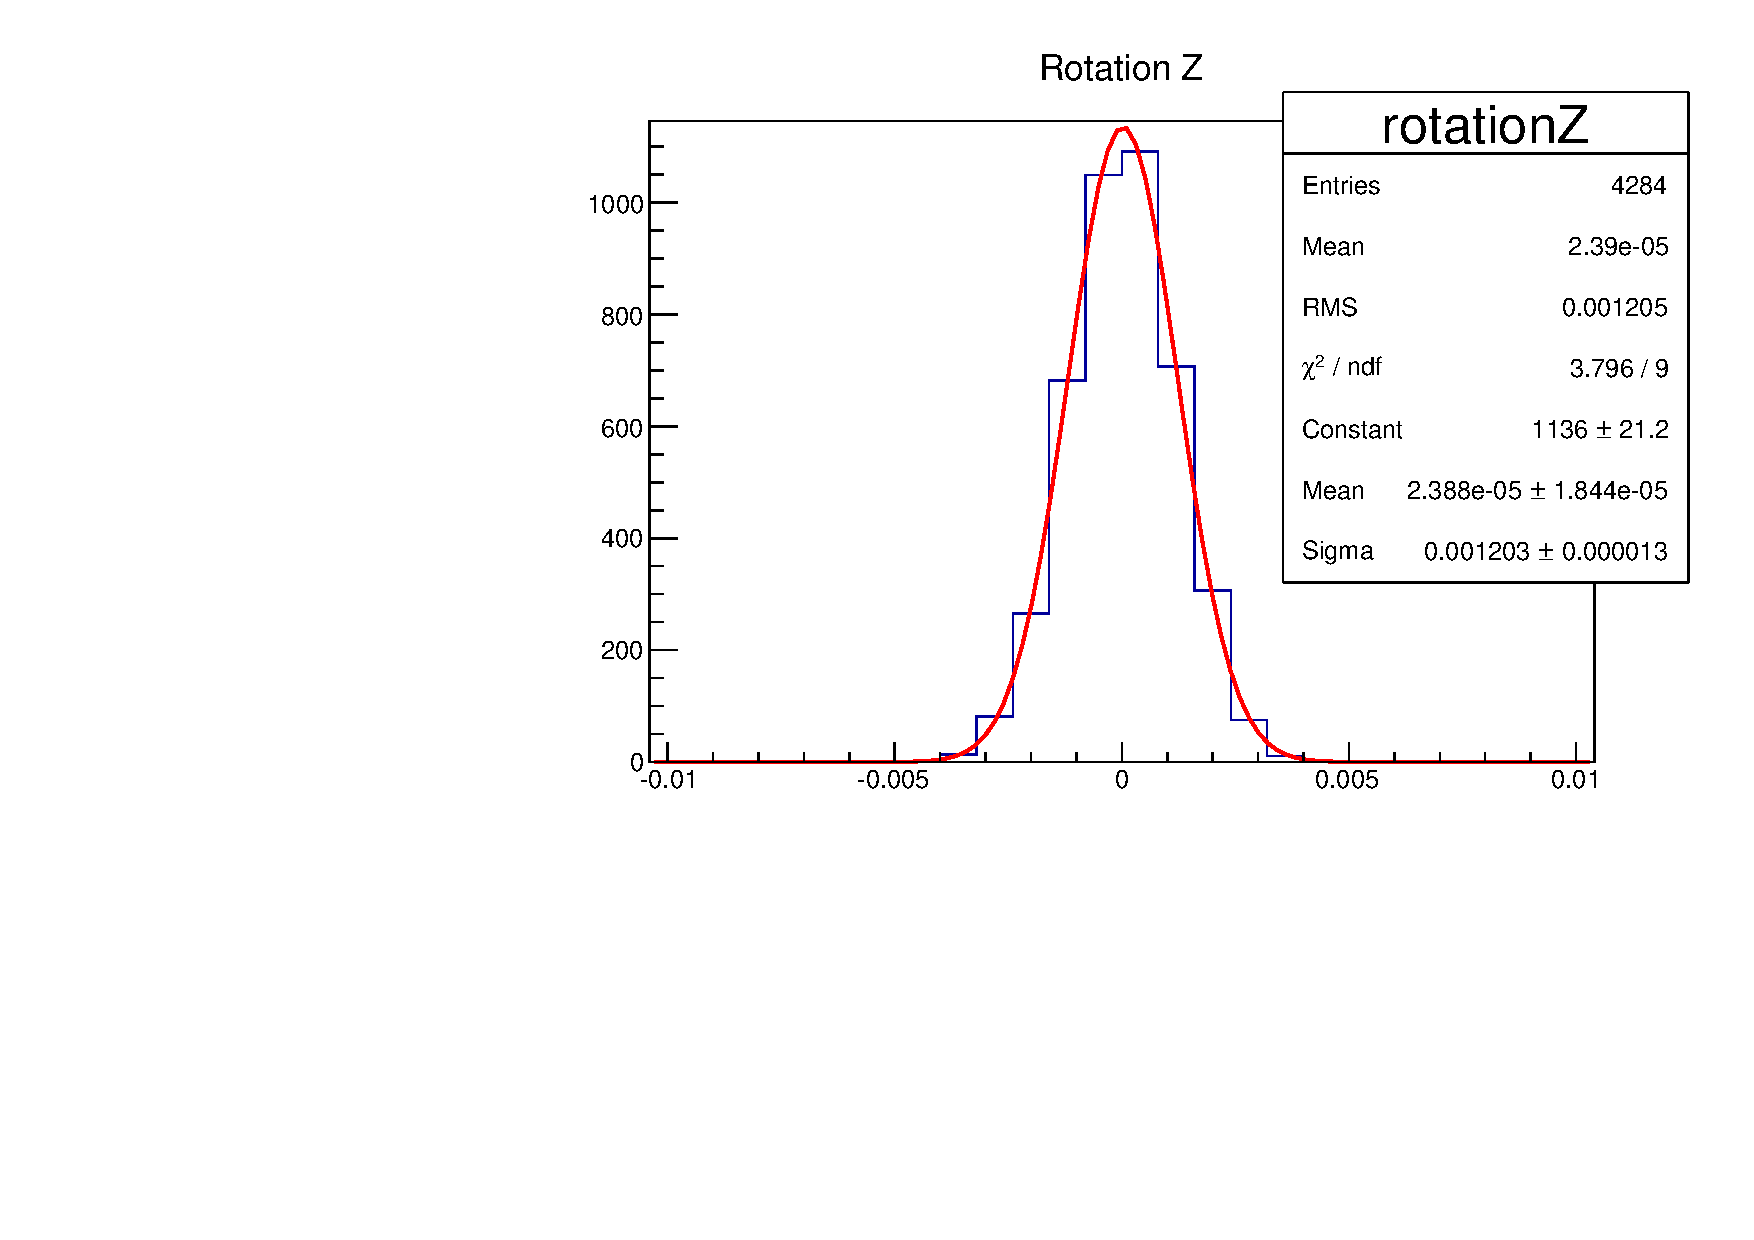
\includegraphics[width=0.80\textwidth]{./figures/Mini_Vexteurs_Alignement_Figures/After_Mini_Rot_Z_1000_Tracks.pdf}
%         }
%      \end{center}
%      \caption{Distributions de param\`etres de l'\'echelle 1 apr\`es alignement}
%      \label{fig:2_500mum}
%    \end{figure}
% 
% %   La figure \ref{fig:MV_After_Mini_Rot_Z} repr\'esente la distribution de l'inclinaison $angleZ$ de l'\'echelle apr\`es alignements. Pour cela, 4284 lots de donn\'ees diff\'erents, comportant chacun 1000 couples de mini-vecteurs, ont \'et\'e minimis\'es. La distribution obtenue est alors ajust\'ee avec une fonction Gaussienne. Cette derni\`ere est centr\'ee sur la valeur $2.4 \, 10^{-5}$ degr\'e et poss\`ede une largeur d'environ $1 \, 10^{-3}$ degr\'e. La valeur $angleZ = 0$ degr\'es est bien retrouv\'ee.
% 
%   \FloatBarrier

%   \begin{figure}[!htb]
%     \begin{center}
%       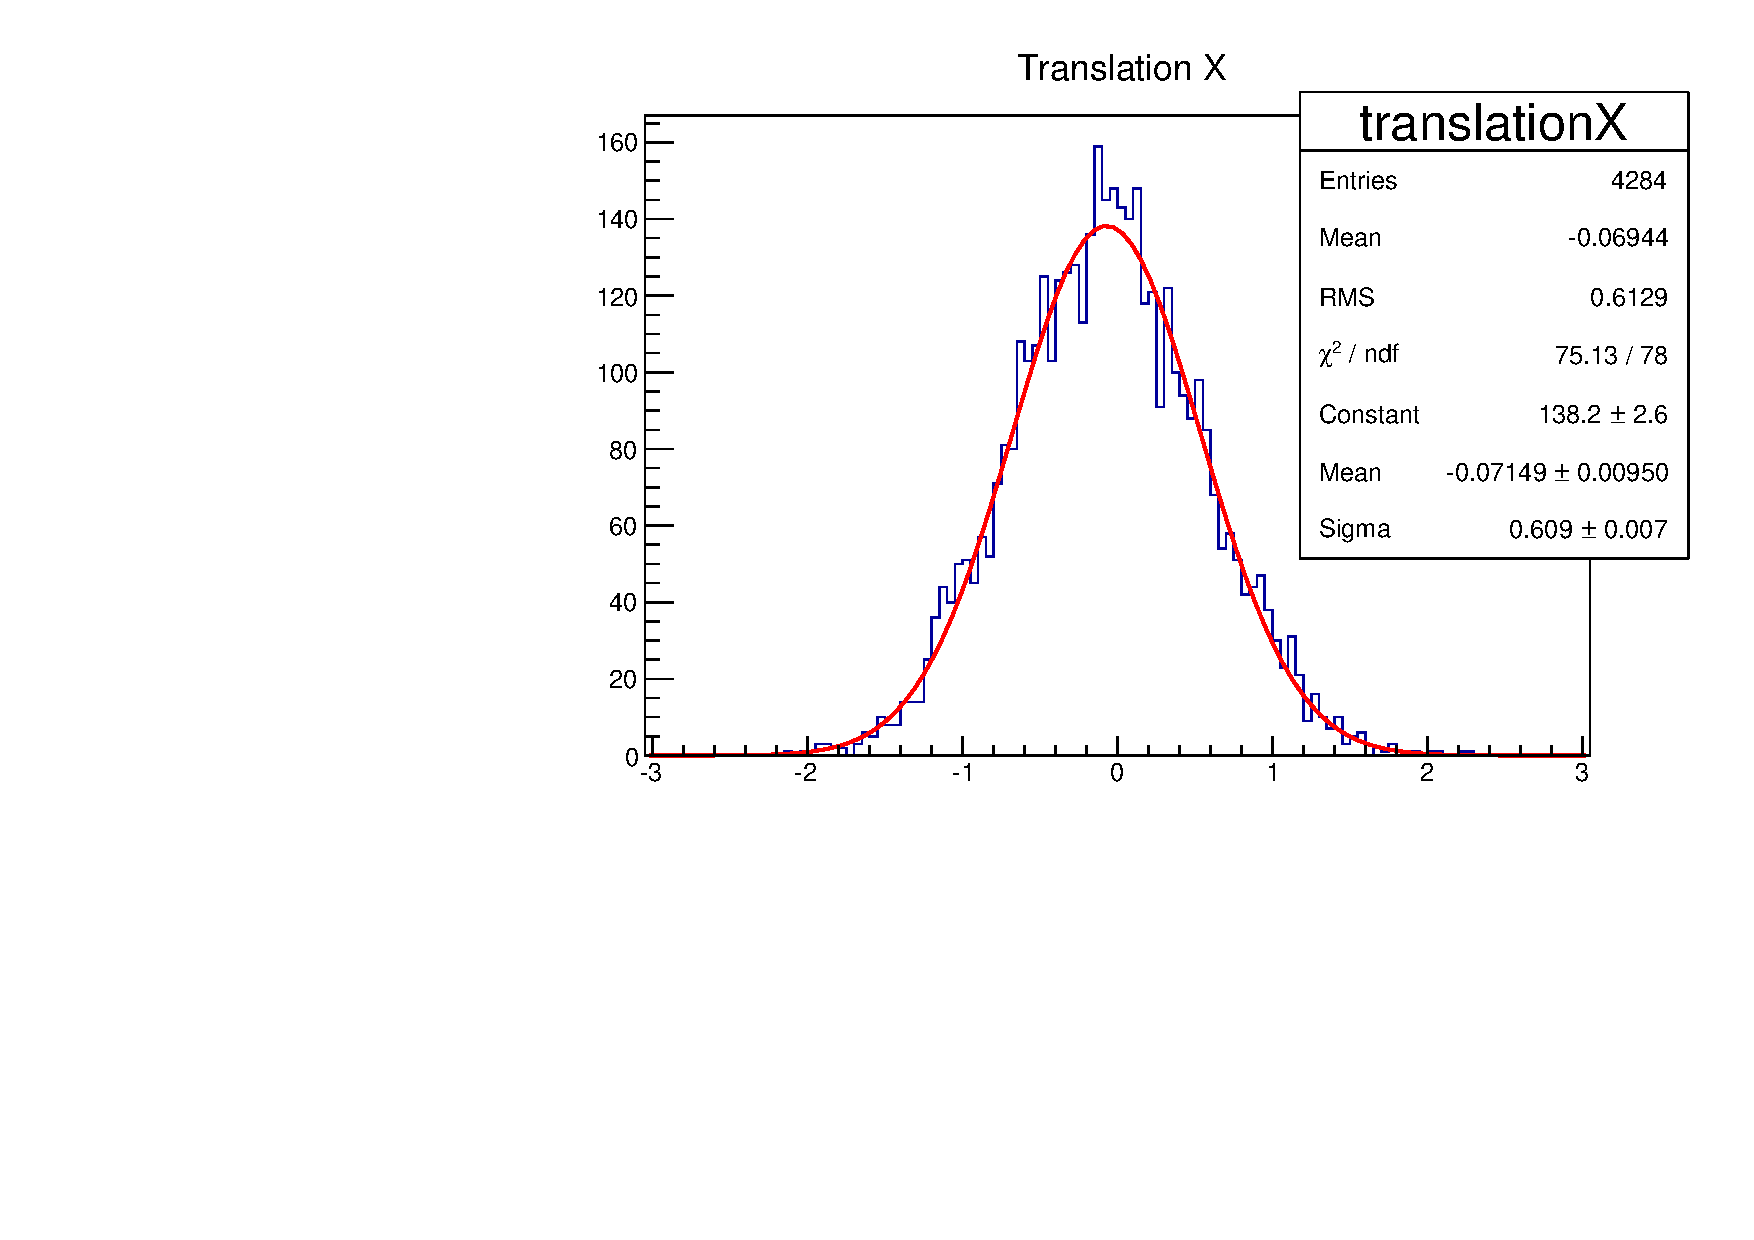
\includegraphics[scale=0.70]{./figures/Mini_Vexteurs_Alignement_Figures/After_Mini_Tr_X_1000_Tracks.pdf}
%       \caption{Distribution de la coordonn\'ee $X1$ du centre de l'\'echelle apr\`es alignements. 4284 lots de donn\'ees diff\'erents ont \'et\'e minimis\'es. Chacun de ces lots comporte 1000 couples de mini-vecteurs. La valeur attendue 0 est retrouv\'ee.}
%       \label{fig:MV_After_Mini_Tr_X}
%     \end{center}
%   \end{figure}

  
%   \begin{figure}[!htb]
%     \begin{center}
%       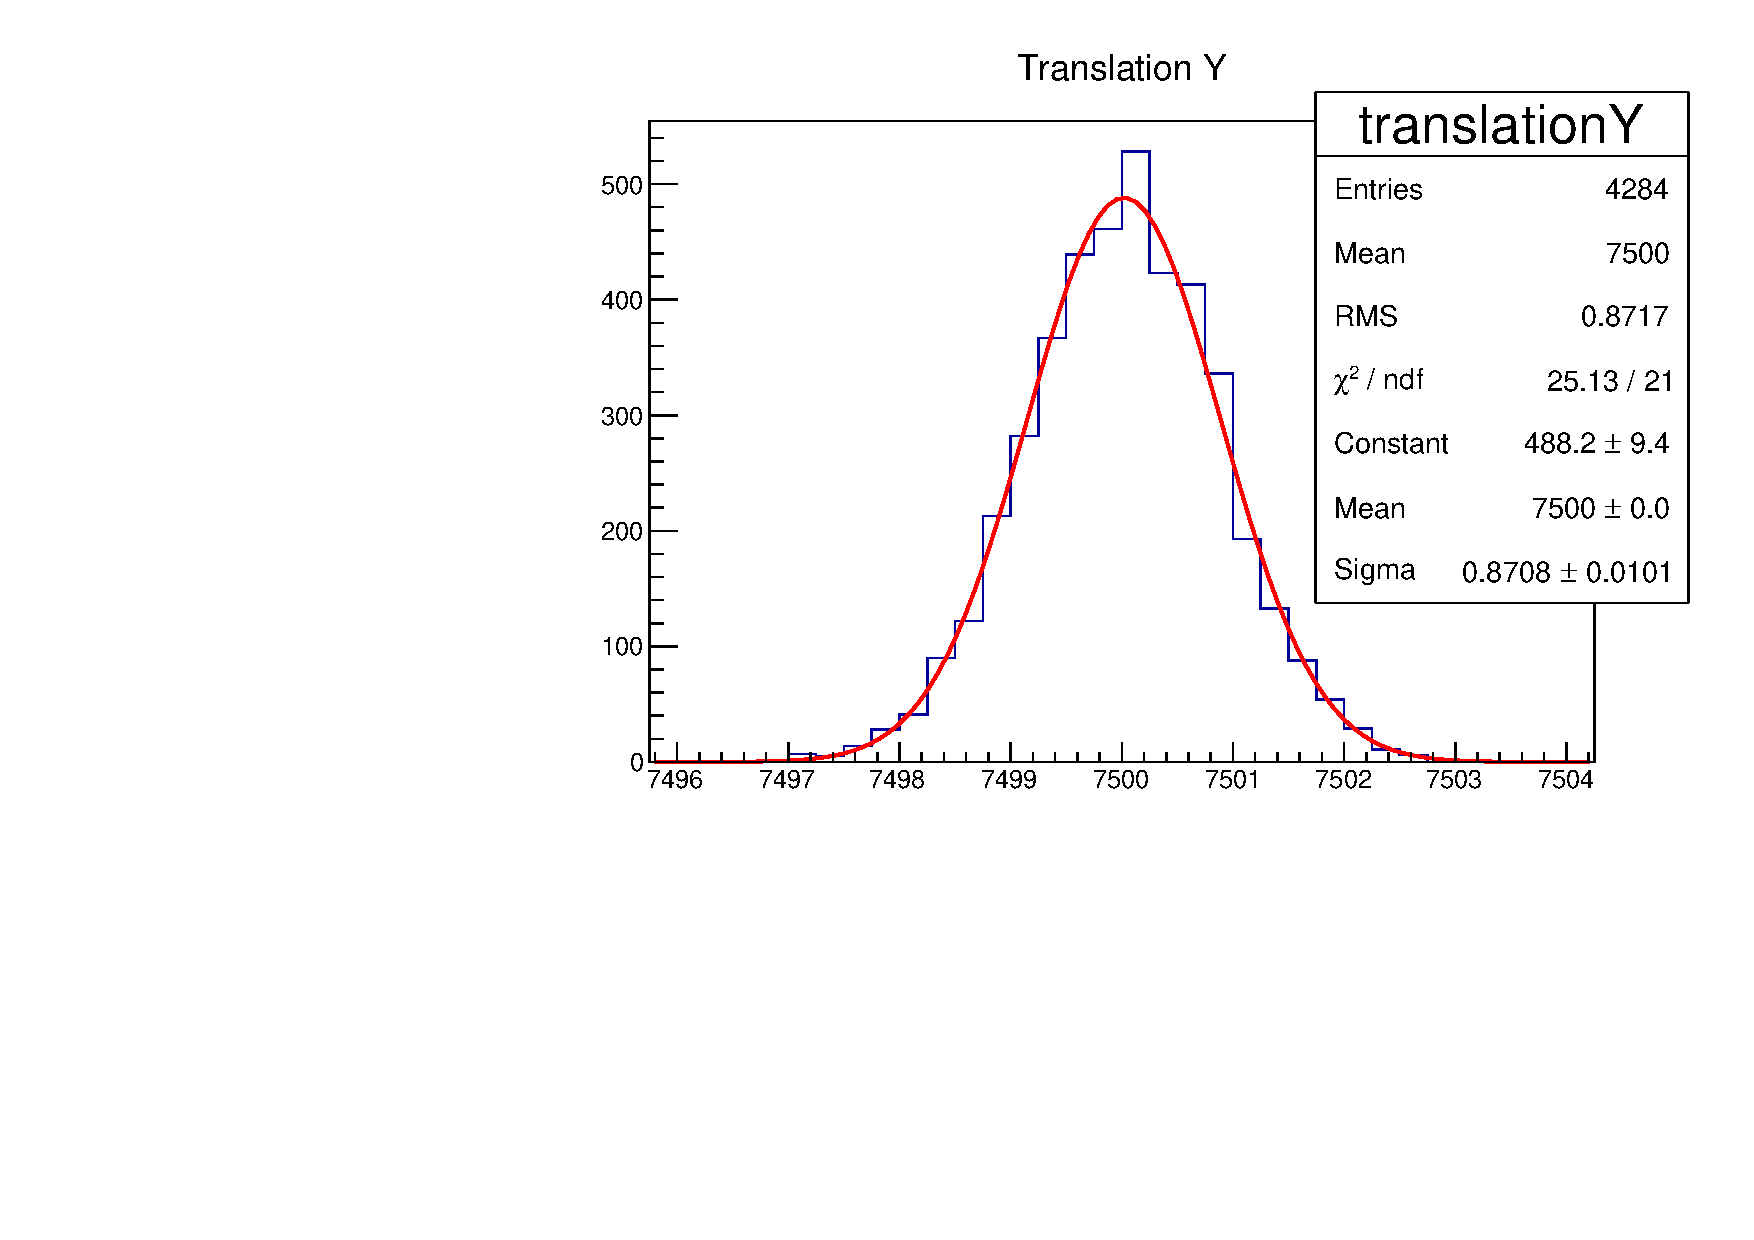
\includegraphics[scale=0.70]{./figures/Mini_Vexteurs_Alignement_Figures/After_Mini_Tr_Y_1000_Tracks.pdf}
%       \caption{Distribution de la coordonn\'ee $Y1$ du centre de l'\'echelle 1 apr\`es alignements. 4284 lots de donn\'ees diff\'erents ont \'et\'e minimis\'es. Chacun de ces lots comporte 1000 couples de mini-vecteurs. La valeur attendue 7500 est retrouv\'ee.}
%       \label{fig:MV_After_Mini_Tr_Y}
%     \end{center}
%   \end{figure}



%   \medskip
%   Conclure \\
%   Biais sans le $\chi^2$ ???
%   Dire pk \'ecart ? epaisseur couche \'epi ???
%   \medskip
  
%   \begin{figure}[!htb]
%     \begin{center}
%       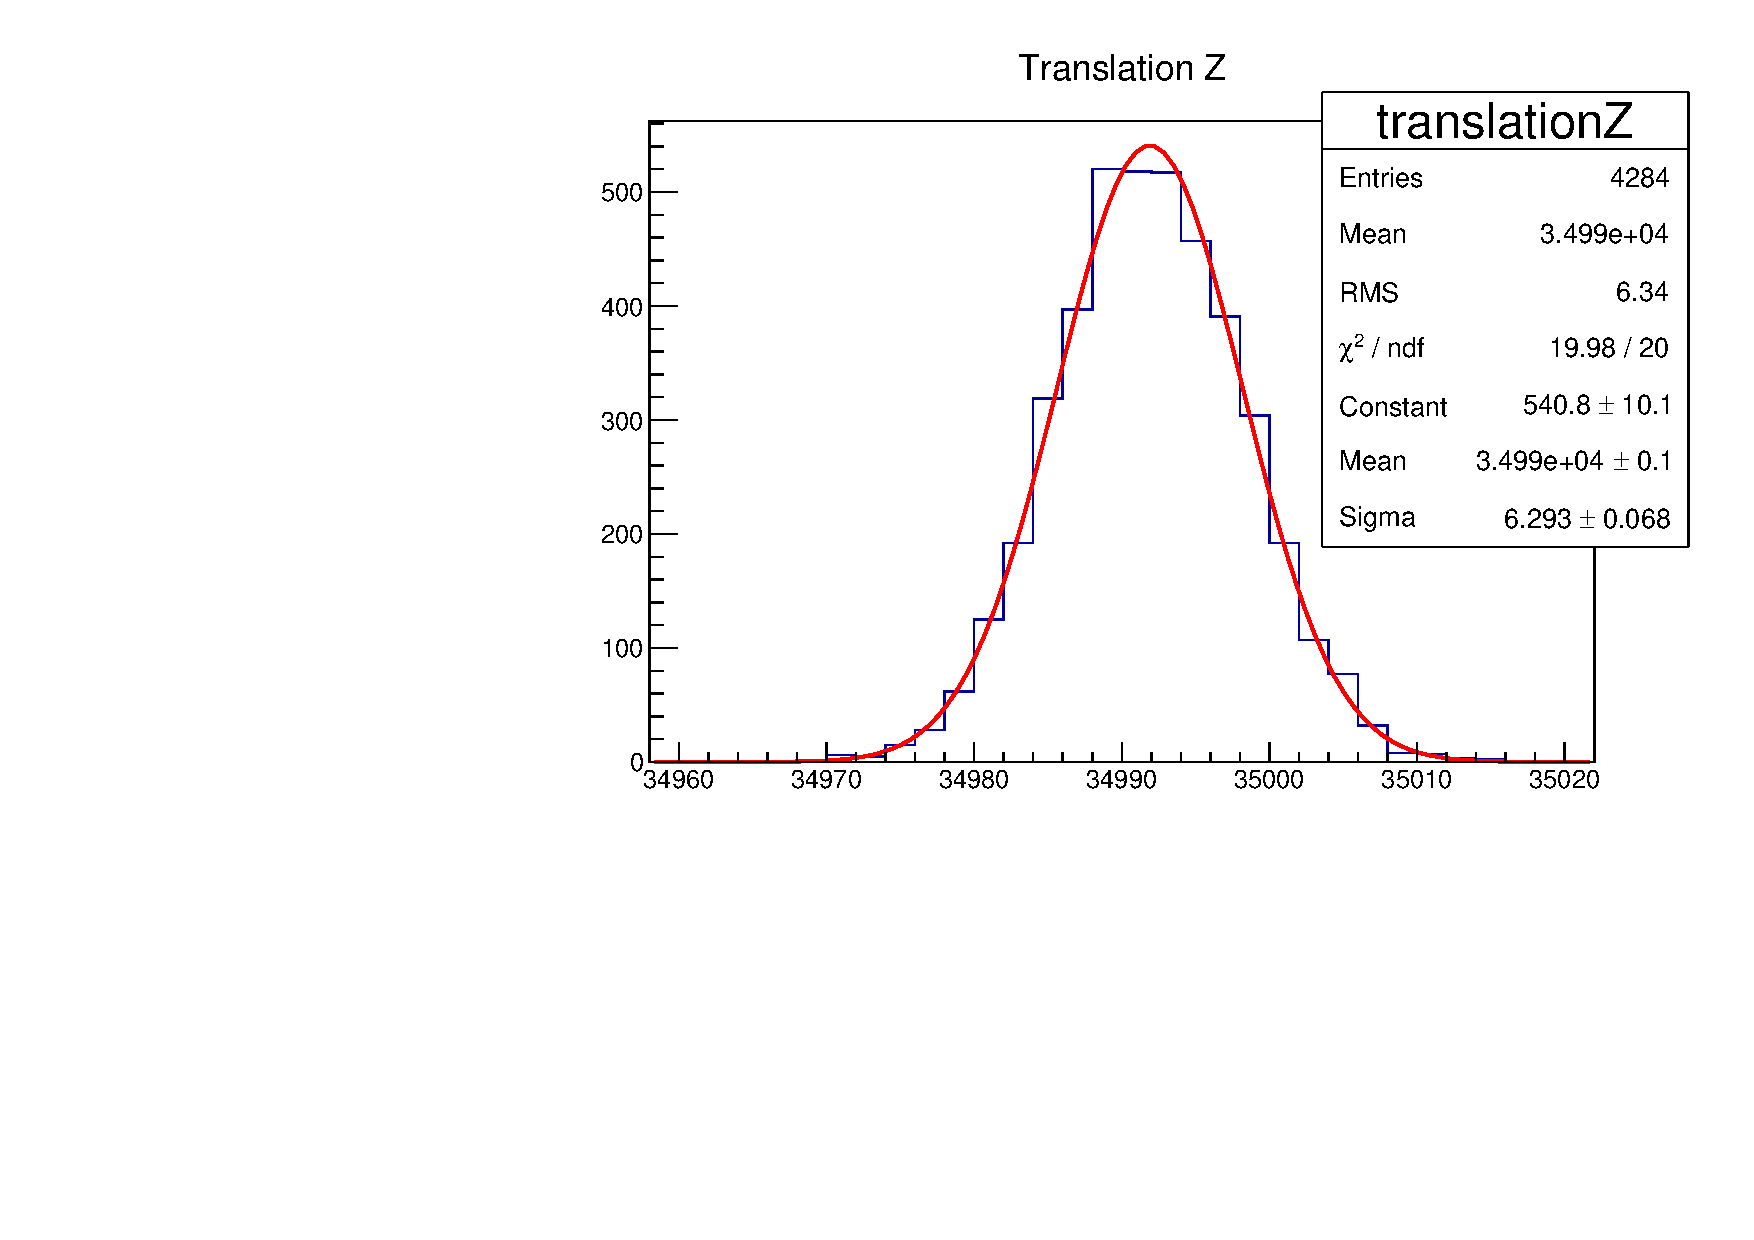
\includegraphics[scale=0.70]{./figures/Mini_Vexteurs_Alignement_Figures/After_Mini_Tr_Z_1000_Tracks.pdf}
%       \caption{Distribution de la coordonn\'ee $Z1$ du centre de l'\'echelle 1 apr\`es alignements. 4284 lots de donn\'ees diff\'erents ont \'et\'e minimis\'es. Chacun de ces lots comporte 1000 couples de mini-vecteurs. La valeur attendue vaut 35000. Un \'ecart de 10 $\mu m$ est observ\'e.}
%       \label{fig:MV_After_Mini_Tr_Z}
%     \end{center}
%   \end{figure}

  
%   \begin{figure}[!htb]
%     \begin{center}
%       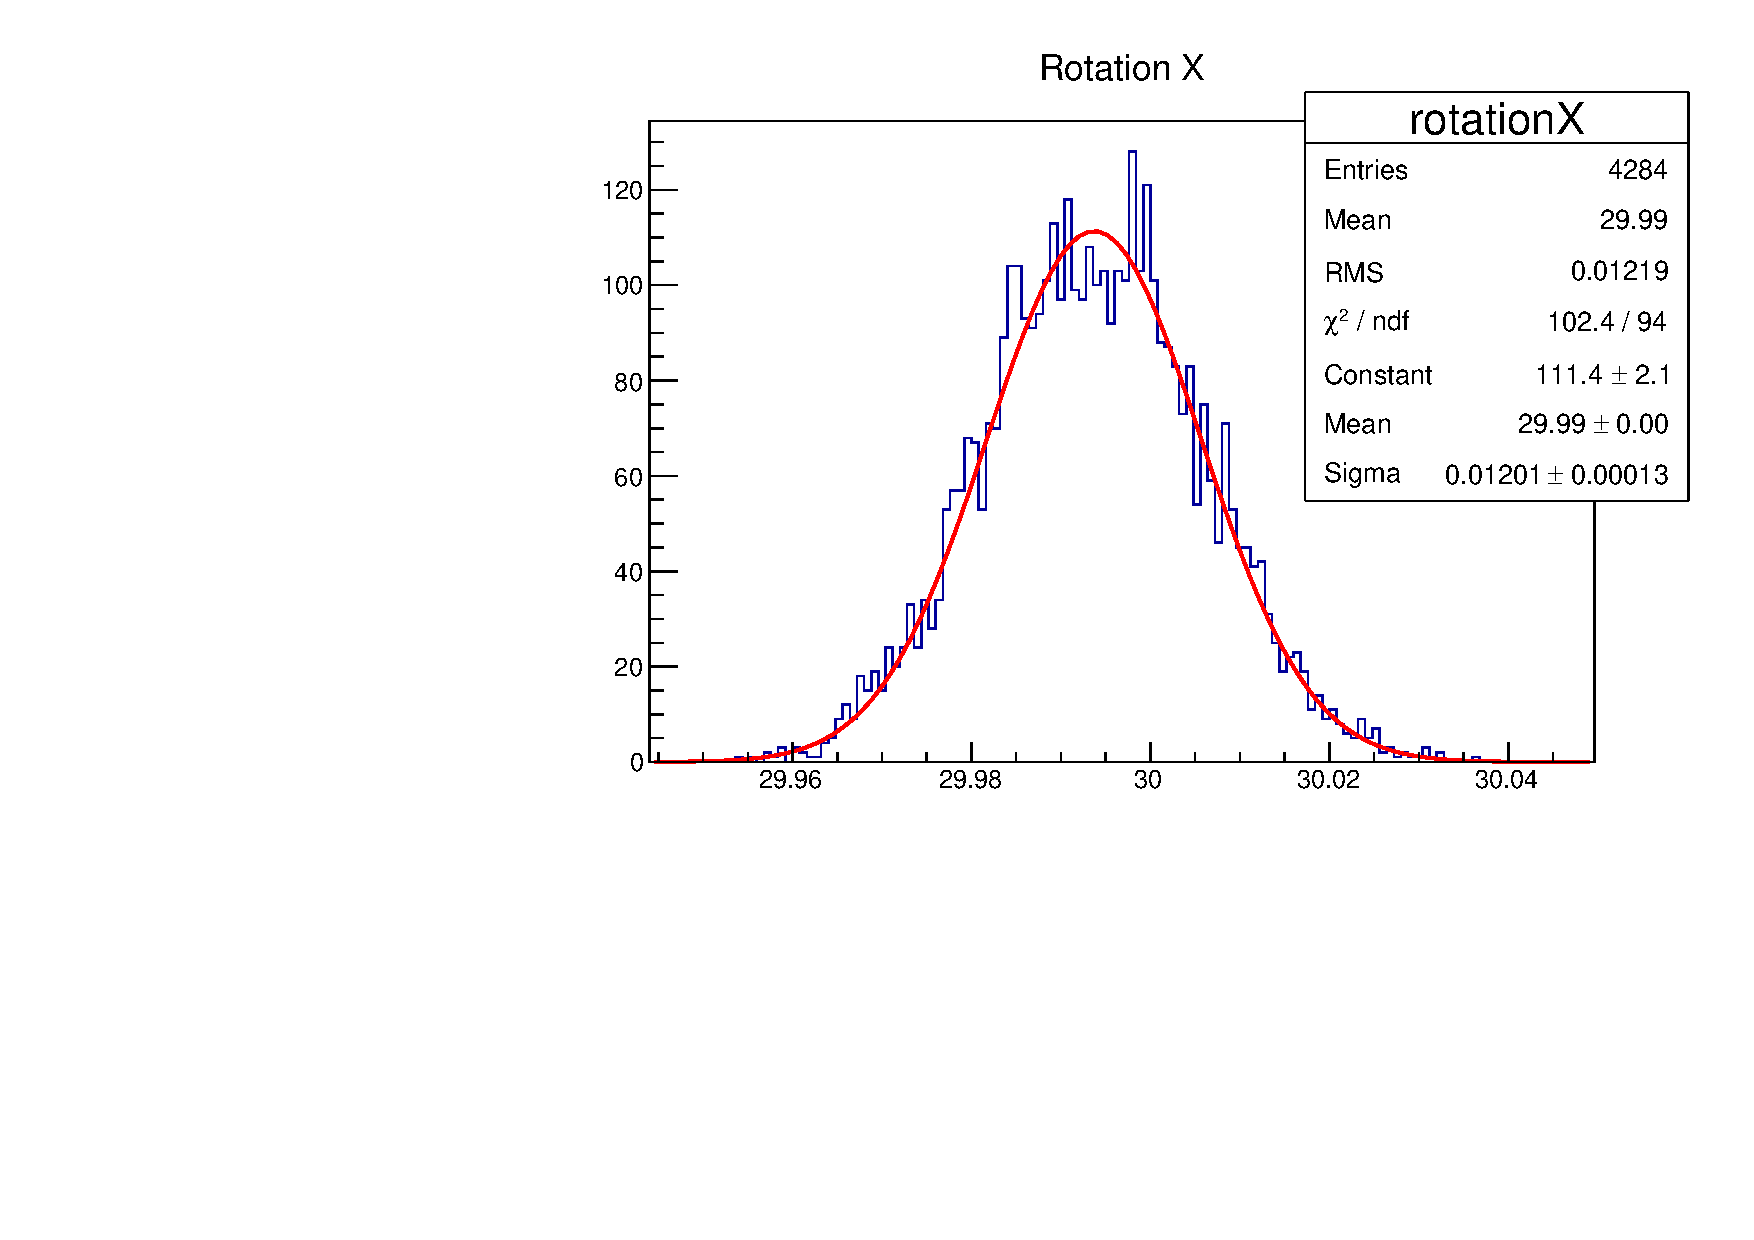
\includegraphics[scale=0.70]{./figures/Mini_Vexteurs_Alignement_Figures/After_Mini_Rot_X_1000_Tracks.pdf}
%       \caption{Distribution de l'inclinaison de l'\'echelle 1 selon son axe $C1X$ apr\`es alignements. 4284 lots de donn\'ees diff\'erents ont \'et\'e minimis\'es. Chacun de ces lots comporte 1000 couples de mini-vecteurs. La valeur entendu 30 degr\'es est retrouv\'ee}
%       \label{fig:MV_After_Mini_Rot_X}
%     \end{center}
%   \end{figure}


  
%   \begin{figure}[!htb]
%     \begin{center}
%       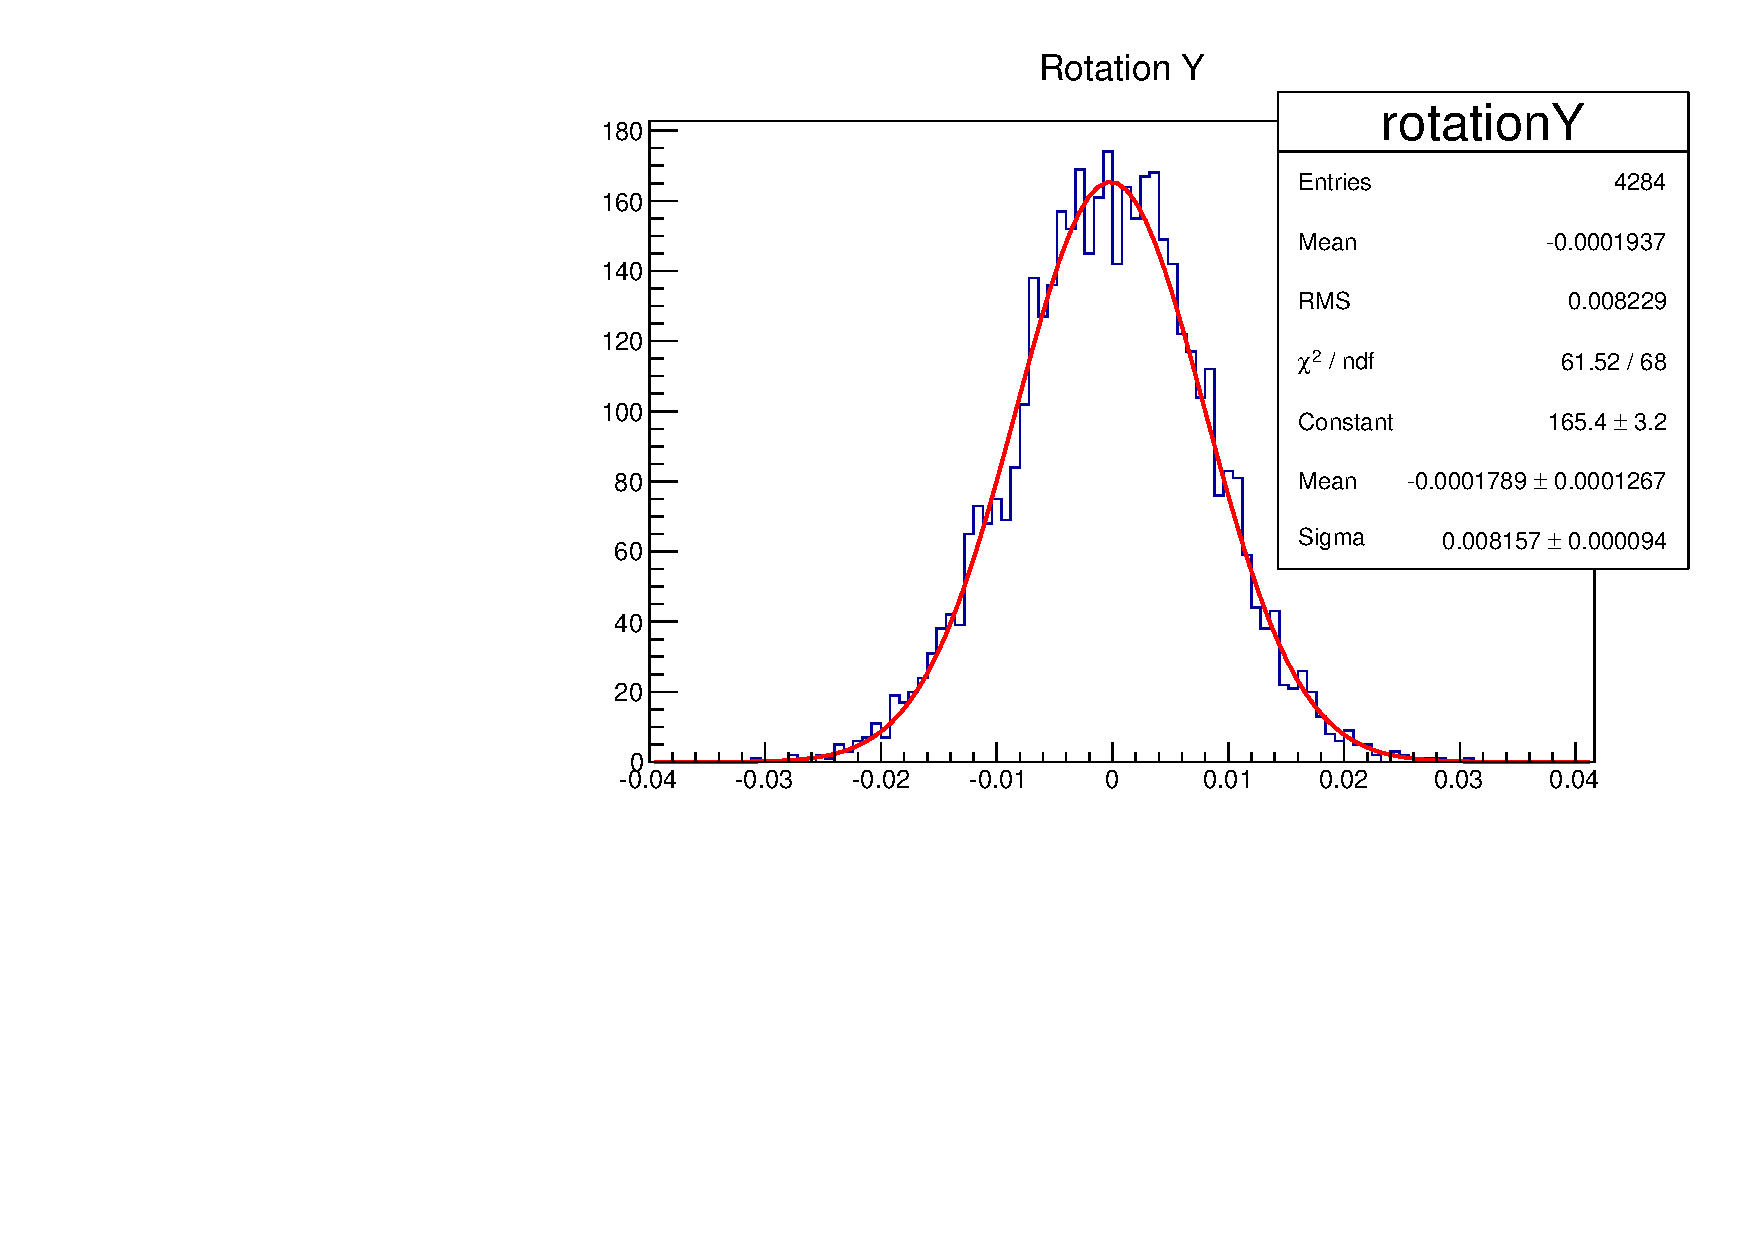
\includegraphics[scale=0.70]{./figures/Mini_Vexteurs_Alignement_Figures/After_Mini_Rot_Y_1000_Tracks.pdf}
%       \caption{Distribution de l'inclinaison de l'\'echelle 1 selon son axe $C1Y$ apr\`es alignements. 4284 lots de donn\'ees diff\'erents ont \'et\'e minimis\'es. Chacun de ces lots comporte 1000 couples de mini-vecteurs. La valeur entendu 0 degr\'e est retrouv\'ee}
%       \label{fig:MV_After_Mini_Rot_Y}
%     \end{center}
%   \end{figure}
  
%   \begin{figure}[!htb]
%     \begin{center}
%       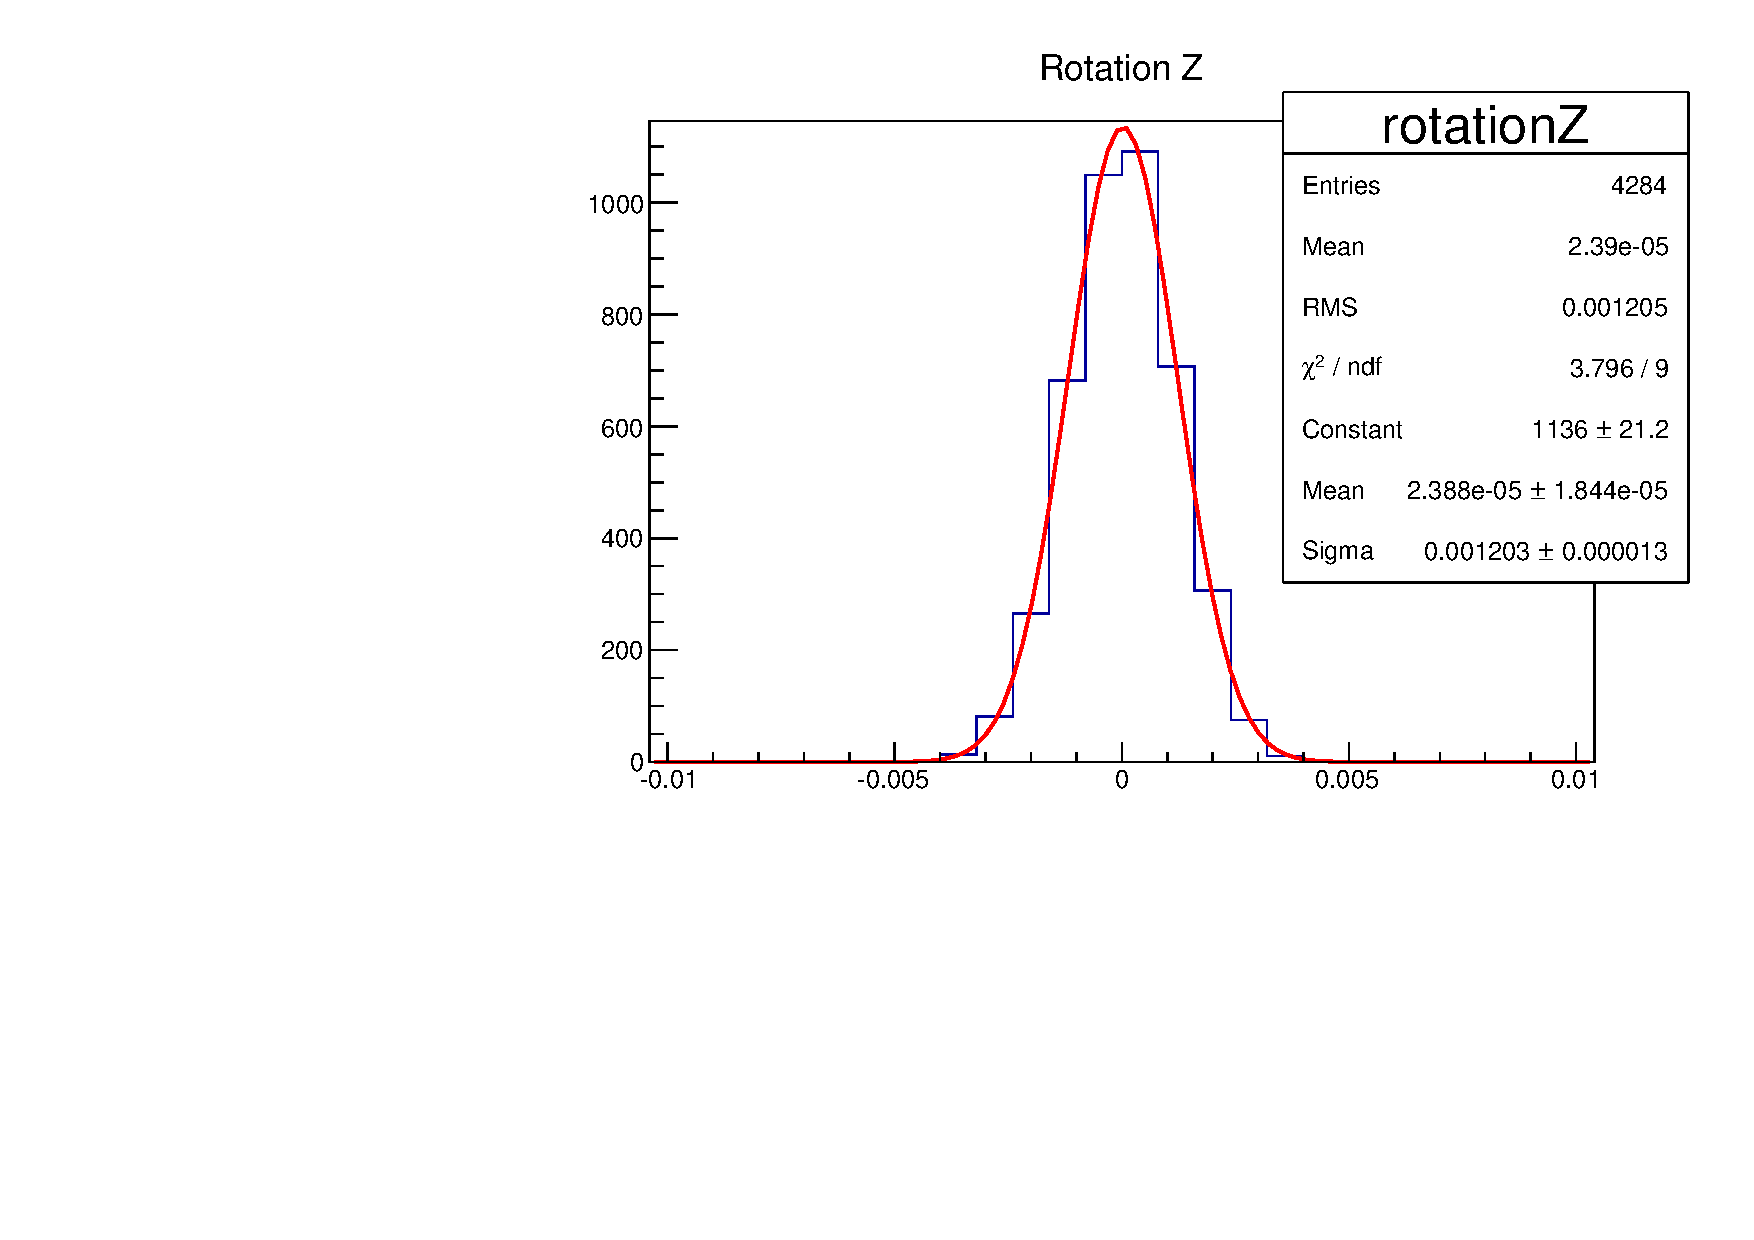
\includegraphics[scale=0.70]{./figures/Mini_Vexteurs_Alignement_Figures/After_Mini_Rot_Z_1000_Tracks.pdf}
%       \caption{Distribution de l'inclinaison de l'\'echelle 1 selon son axe $C1Z$ apr\`es alignements. 4284 lots de donn\'ees diff\'erents ont \'et\'e minimis\'es. Chacun de ces lots comporte 1000 couples de mini-vecteurs. La valeur entendu 0 degr\'e est retrouv\'ee}
%       \label{fig:MV_After_Mini_Rot_Z}
%     \end{center}
%   \end{figure}
  
%   \subsubsection{Pr\'ecision de la m\'ethode en fonction de la statistique}

%   Nous allons \`a pr\'esent \'etudier la m\'ethode d'alignement avec mini-vecteurs en fonction de la statistique disponible. La m\^eme configuration que pr\'ec\'edemment a \'et\'e utilis\'ee. Afin d'\'etudier la pr\'ecision de cette m\'ethode d'alignement en fonction de la statistique, les courbes d\'ecrites en section \ref{sect:Resultats_alignement_MV} sont trac\'ees pour des \'echantillons de donn\'ees comportant 250, 500, 1000, 2500, 5000, 10000 et 20000 couples de mini-vecteurs. L'\'etude s'est arr\^eté \`a 20 000 couples de mini-vecteurs en raison de la m\'emoire vive occup\'ee et du nombre de donn\'ees simul\'ees n\'ecessaires.
%   
%   \medskip
%   
%   Pour notre \'etude, on notera la moyenne de la distribution des param\`etres apr\`es alignement $M_i$ et leur largeur $\sigma_i$. De plus, on appelle $P_i$ les valeurs des param\`etres de l'\'echelle \`a aligner telle qu'elles sont renseign\'ees dans la simulation Monte-Carlo. (Cela correspond \`a un alignement parfait). Les d\'eviations \`a la valeur des param\`etres Monte-Carlo seront exprim\'e par la variable :  
%   
%   
%   \begin{equation}
%    \Delta M_i = M_i - P_i
%   \end{equation}
% 
%   On étudiera ici, les variations de $\Delta M_i$  et des largeurs $\sigma_i$ en fonction de la statistique. Les résultats obtenues pour chaque param\`etre de l'\'echelle sont visibles en figures \ref{fig:Precision_0}, \ref{fig:Precision_1} et \ref{fig:Precision_2}.
  
%   \medskip
% 
%    La figure \ref{fig:MV_prec_Tr_X1} indique les valeurs de $\Delta M$ pour la coordonn\'ee $X1$ du centre de l'\'echelle \`a aligner, apr\`es alignement ; et les valeurs $\sigma$ de la largeur de la distribution du param\`etre $X1$ apr\`es alignement. Quelque soit le nombre de couples de mini-vecteurs, la valeur de $\Delta M$ reste fixe et vaut environ $-0.07 \, \mu m$. La largeur de la distribution des $X1$ après alignement vaut environ $1.15 \, \mu m$ pour 500 couples de mini-vecteurs et descend \`a $0.15 \, \mu m$ pour 20 000 couples de mini-vecteurs. La pente de la courbe d\'ecrivant la largeur devient de plus en plus faible \`a mesure que l'on rajoute des couples de mini-vecteurs. La largeur obtenue semble se stabiliser pour un nombre de couples de mini-vecteurs sup\'erieur ou \'egal \`a 20 000. La largeur repr\'esent\'ee ici repr\'esente la r\'esolution de la m\'ethode d'alignement pour la coordonn\'ee $X1$. Ainsi, d\`es l'obtention de 1000 couples de mini-vecteurs bien associ\'es, la pr\'ecision de l'alignement selon cette coordonn\'ee est meilleure que $1 \mu m$. Pour 10 000 couples de mini-vecteurs bien associ\'es, la pr\'ecision atteint 0.2 $\mu m$.
% 
%   \medskip
%   
%    La figure \ref{fig:MV_prec_Tr_Y1} indique les valeurs de $\Delta M$ pour la coordonn\'ee $Y1$ du centre de l'\'echelle \`a aligner, apr\`es alignement ; et les valeurs $\sigma$ de la largeur de la distribution du param\`etre $Y1$ apr\`es alignement. Quelque soit le nombre de couples de mini-vecteurs, la valeur de $\Delta M$ reste fixe et vaut environ $0 \mu m$. La largeur de la distribution des $Y1$ après alignement vaut environ $1.7 \, \mu m$ pour 500 couples de mini-vecteurs et descend \`a $0.20 \, \mu m$ pour 20 000 couples de mini-vecteurs. La pente de la courbe d\'ecrivant la largeur devient de plus en plus faible \`a mesure que l'on rajoute des couples de mini-vecteurs. La largeur obtenue semble se stabiliser pour un nombre de couples de mini-vecteurs sup\'erieur ou \'egal \`a 20 000. La largeur repr\'esent\'ee ici repr\'esente la r\'esolution de la m\'ethode d'alignement pour la coordonn\'ee $Y1$. Ainsi, d\`es l'obtention de 1000 couples de mini-vecteurs bien associ\'es, la pr\'ecision de l'alignement selon cette coordonn\'ee est meilleure que $1 \mu m$. Pour 10 000 couples de mini-vecteurs bien associ\'es, la pr\'ecision atteint 0.3 $\mu m$.
   
%   \medskip
%   
%    La figure \ref{fig:MV_prec_Tr_Z1} indique les valeurs de $\Delta M$ pour la coordonn\'ee $Z1$ du centre de l'\'echelle \`a aligner, apr\`es alignement ; et les valeurs $\sigma$ de la largeur de la distribution du param\`etre $Z1$ apr\`es alignement. Quelque soit le nombre de couples de mini-vecteurs, la valeur de $\Delta M$ reste fixe et vaut environ $-8 \mu m$. La largeur de la distribution des $Z1$ après alignement vaut environ $12.5 \, \mu m$ pour 500 couples de mini-vecteurs et descend \`a environ $1.75 \, \mu m$ pour 20 000 couples de mini-vecteurs. La pente de la courbe d\'ecrivant la largeur devient de plus en plus faible \`a mesure que l'on rajoute des couples de mini-vecteurs. La largeur obtenue semble se stabiliser pour un nombre de couples de mini-vecteurs sup\'erieur ou \'egal \`a 20 000.
%    
%    \medskip
%    Biais observ\'e ... Dire pourquoi ca coince ^^' pour Oz ...
%    \medskip
%   
%    La figure \ref{fig:MV_prec_Rot_X} indique les valeurs de $\Delta M$ pour l'inclinaison $angleX$ de l'\'echelle \`a aligner, apr\`es alignement ; et les valeurs $\sigma$ de la largeur de la distribution du param\`etre $angleX$ apr\`es alignement. Quelque soit le nombre de couples de mini-vecteurs, la valeur de $\Delta M$ reste fixe et vaut environ $7 \, 10^{-3}$ degr\'es. La largeur de la distribution des $angleX$ après alignement vaut environ $2.4 \, 10^{-2}$ degr\'e pour 500 couples de mini-vecteurs et descend \`a environ $3 \, 10^{-3}$ degr\'e pour 20 000 couples de mini-vecteurs. La pente de la courbe d\'ecrivant la largeur devient de plus en plus faible \`a mesure que l'on rajoute des couples de mini-vecteurs. La largeur obtenue semble se stabiliser pour un nombre de couples de mini-vecteurs sup\'erieur ou \'egal \`a 20 000. La pr\'ecision obtenue ici est remarquable puisque d\`es 500 couples de mini-vecteurs bien associ\'es la pr\'ecision sur l'inclinaison de l'\'echelle selon son axe $C1X$ est de $2.5 \, 10^{-2}$ degr\'e. Elle atteint moins de $5 \, 10^{-3}$ degr\'e \`a partir de 10000 couples de mini-vecteurs bien associ\'es.
%    
%    \medskip
%   
%    La figure \ref{fig:MV_prec_Rot_Y} indique les valeurs de $\Delta M$ pour l'inclinaison $angleY$ de l'\'echelle \`a aligner, apr\`es alignement ; et les valeurs $\sigma$ de la largeur de la distribution du param\`etre $angleY$ apr\`es alignement. Quelque soit le nombre de couples de mini-vecteurs, la valeur de $\Delta M$ reste fixe et vaut environ $-1 \, 10^{-3}$ degr\'es. La largeur de la distribution des $angleY$ après alignement vaut environ $1.6 \, 10^{-2}$ degr\'e pour 500 couples de mini-vecteurs et descend \`a environ $2 \, 10^{-3}$ degr\'e pour 20 000 couples de mini-vecteurs. La pente de la courbe d\'ecrivant la largeur devient de plus en plus faible \`a mesure que l'on rajoute des couples de mini-vecteurs. La largeur obtenue semble se stabiliser pour un nombre de couples de mini-vecteurs sup\'erieur ou \'egal \`a 20 000. La pr\'ecision obtenue ici est aussi remarquable puisque d\`es 500 couples de mini-vecteurs bien associ\'es la pr\'ecision sur l'inclinaison de l'\'echelle selon son axe $C1Y$ est de $1.6 \, 10^{-2}$ degr\'e. Elle atteint moins de $3 \, 10^{-3}$ degr\'e \`a partir de 10000 couples de mini-vecteurs bien associ\'es.
% 
%    \medskip
%   
%    La figure \ref{fig:MV_prec_Rot_Z} indique les valeurs de $\Delta M$ pour l'inclinaison $angleZ$ de l'\'echelle \`a aligner, apr\`es alignement ; et les valeurs $\sigma$ de la largeur de la distribution du param\`etre $angleZ$ apr\`es alignement. Quelque soit le nombre de couples de mini-vecteurs, la valeur de $\Delta M$ reste fixe et vaut environ $1 \, 10^{-5}$ degr\'es. La largeur de la distribution des $angleZ$ après alignement vaut environ $2.4 \, 10^{-3}$ degr\'e pour 500 couples de mini-vecteurs et descend \`a environ $3.5 \, 10^{-4}$ degr\'e pour 20 000 couples de mini-vecteurs. La pente de la courbe d\'ecrivant la largeur devient de plus en plus faible \`a mesure que l'on rajoute des couples de mini-vecteurs. La largeur obtenue se stabilise pour un nombre de couples de mini-vecteurs sup\'erieur ou \'egal \`a 20 000. La pr\'ecision sur l'inclinaison de l'\'echelle selon son axe $C1Z$ est inf\'erieure \`a $2.5 \, 10^{-3}$ degr\'e d\`es 500 couples de mini-vecteurs bien associ\'es. Elle atteint moins de $5 \, 10^{-4}$ degr\'e \`a partir de 10000 couples de mini-vecteurs bien associ\'es.
%    
%    \begin{figure}[htb!]
%      \begin{center}
%         \subfigure[En vert : \'ecart \`a la valeur Monte-Carlo de la valeur moyenne de la distribution du param\`etre $X1$ apr\`es alignement, en fonction de la statistique. En rouge : largeur de la distribution du param\`etre $X1$ apr\`es alignement, en fonction de la statistique.]{
%             \label{fig:MV_prec_Tr_X1}
%             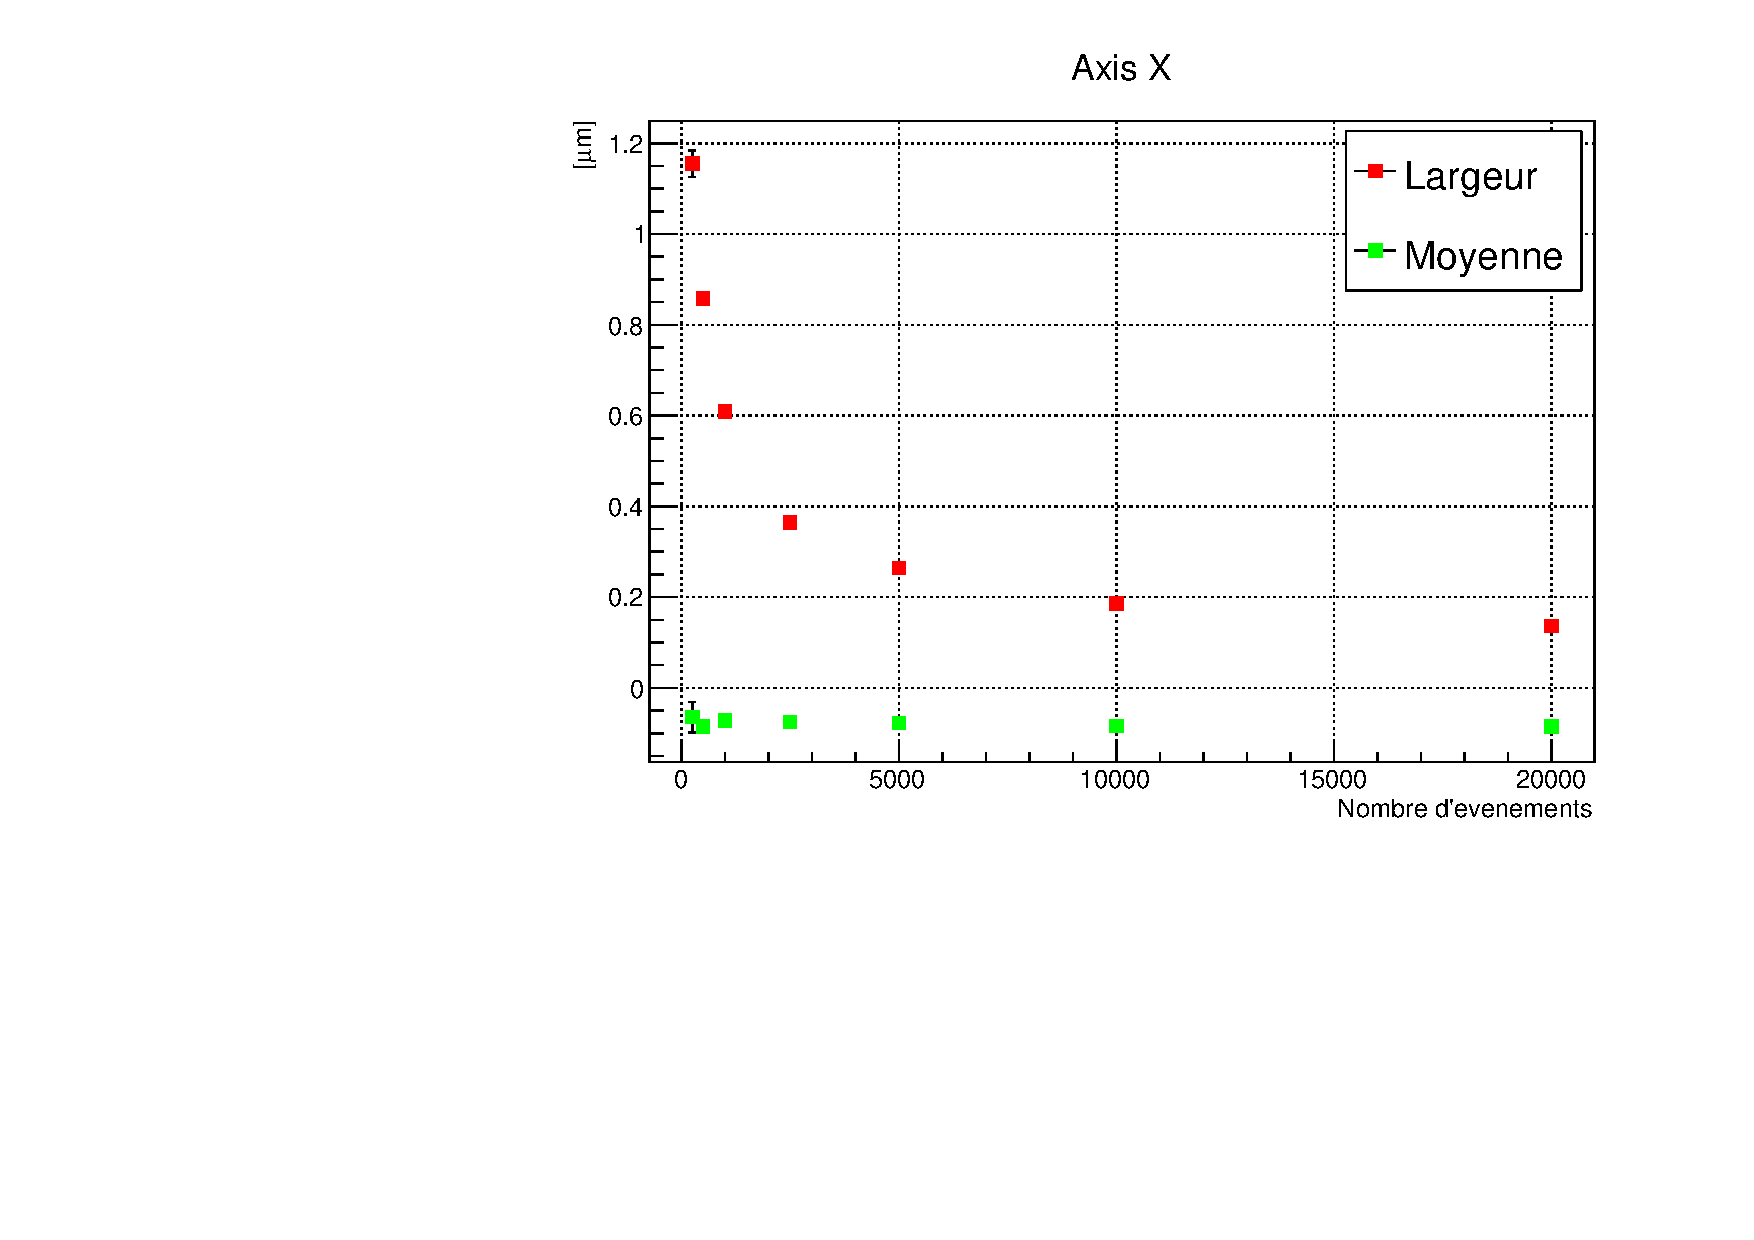
\includegraphics[width=0.78\textwidth]{./figures/Mini_Vexteurs_Alignement_Figures/precision_axe_X.pdf}
%         }
%         \subfigure[En vert : \'ecart \`a la valeur Monte-Carlo de la valeur moyenne de la distribution du param\`etre $Y1$ apr\`es alignement, en fonction de la statistique. En rouge : largeur de la distribution du param\`etre $Y1$ apr\`es alignement, en fonction de la statistique.]{
%            \label{fig:MV_prec_Tr_Y1}
%            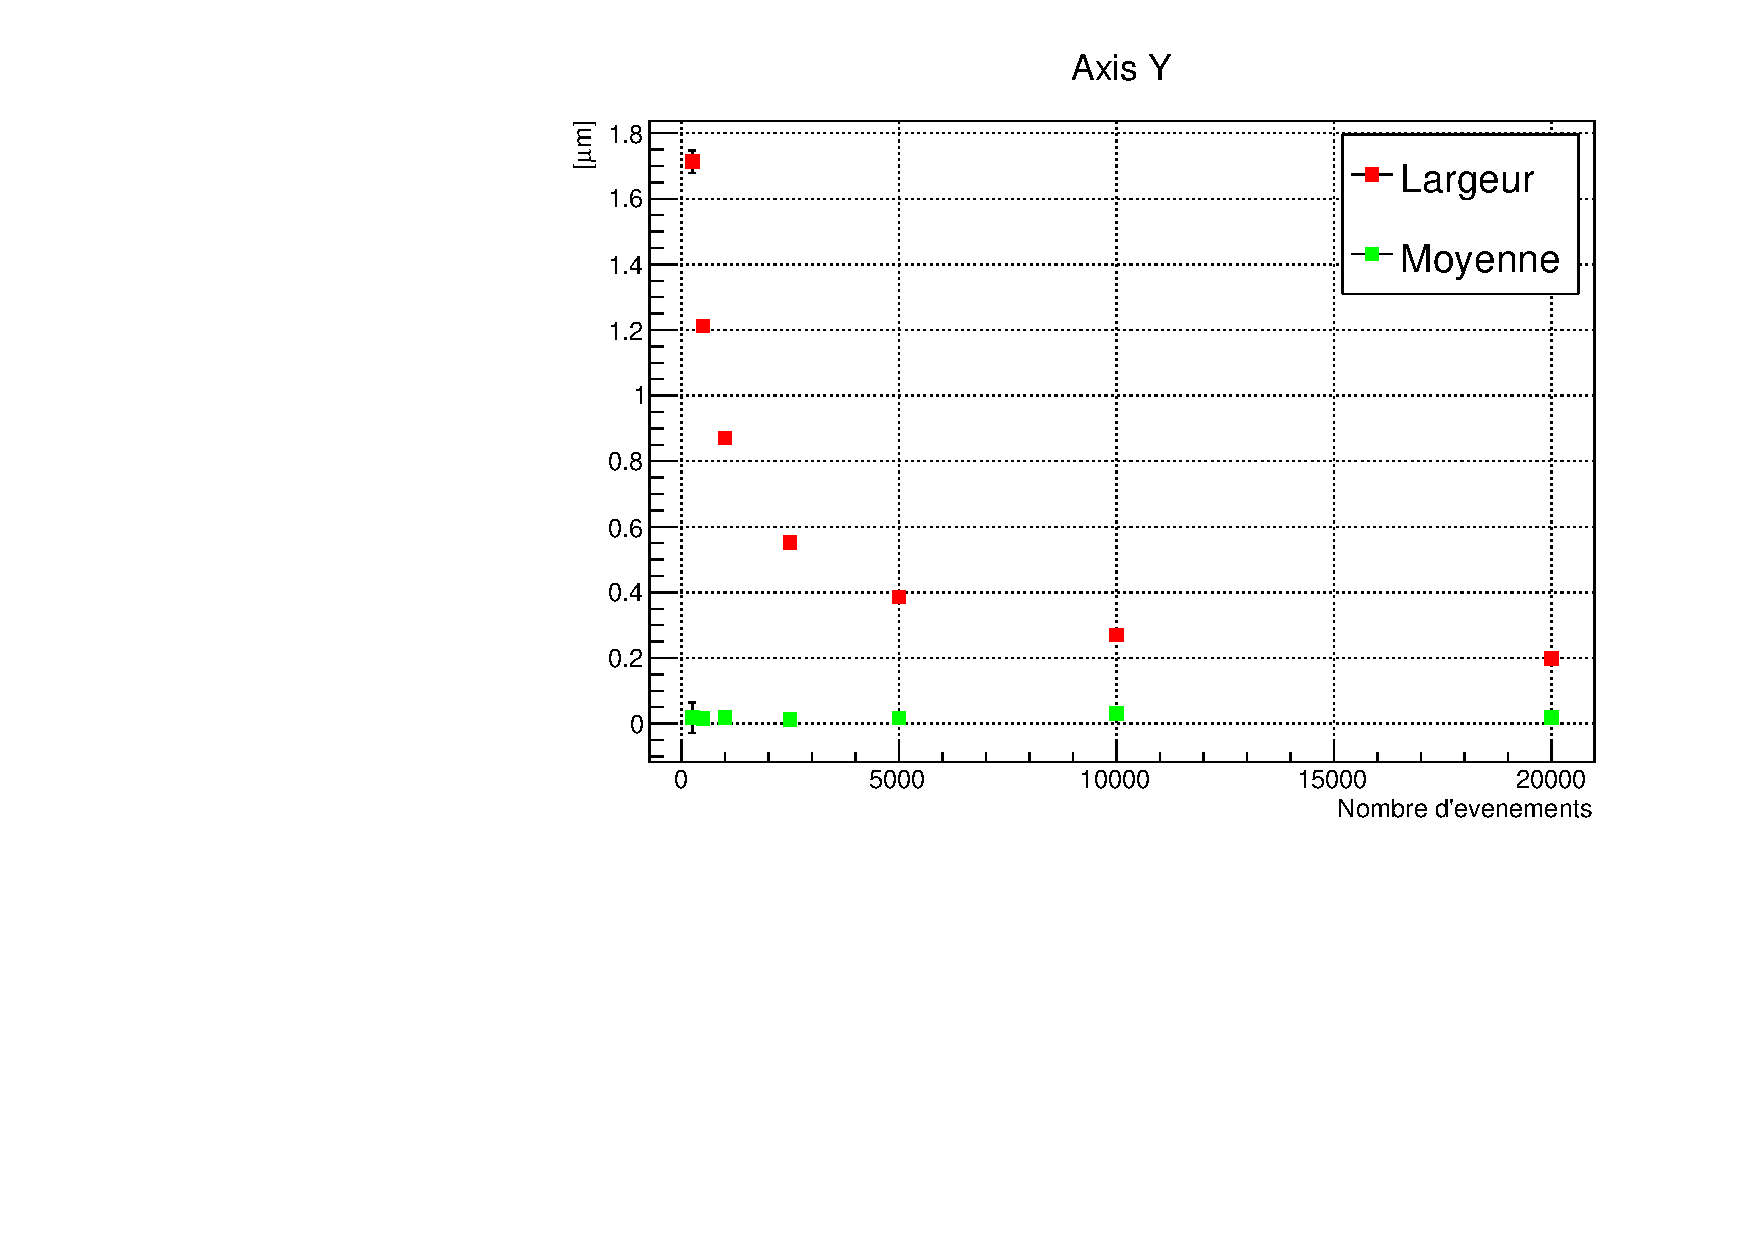
\includegraphics[width=0.78\textwidth]{./figures/Mini_Vexteurs_Alignement_Figures/precision_axe_Y.pdf}
%         }
%      \end{center}
%      \caption{Performances de la m\'ethode d'alignement avec mini-vecteur en fonction de la statistique utilis\'ee}
%      \label{fig:Precision_0}
%    \end{figure}
%   
%    \begin{figure}[htb!]
%      \begin{center}
%         \subfigure[En vert : \'ecart \`a la valeur Monte-Carlo de la valeur moyenne de la distribution du param\`etre $Z1$ apr\`es alignement, en fonction de la statistique. En rouge : largeur de la distribution du param\`etre $Z1$ apr\`es alignement, en fonction de la statistique.]{
%             \label{fig:MV_prec_Tr_Z1}
%             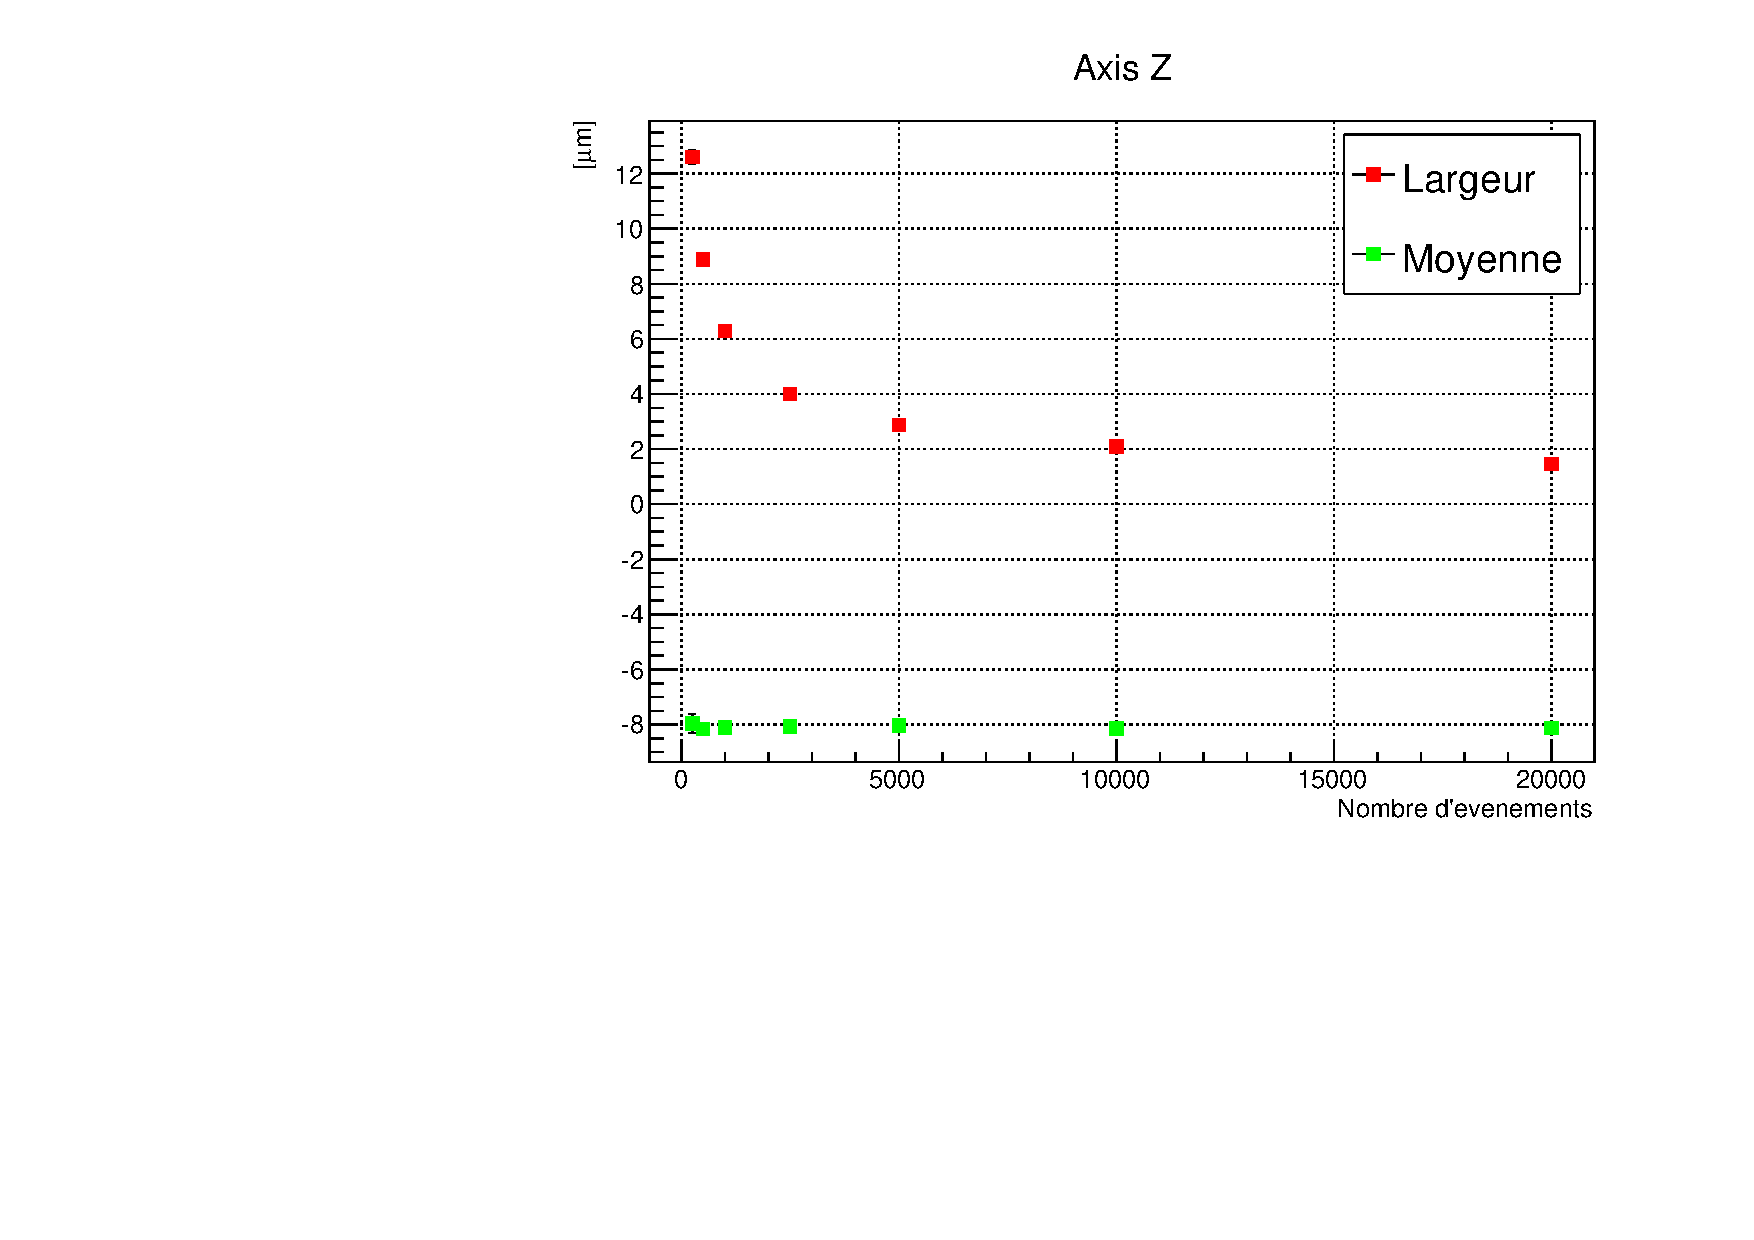
\includegraphics[width=0.78\textwidth]{./figures/Mini_Vexteurs_Alignement_Figures/precision_axe_Z.pdf}
%         }
%         \subfigure[En vert : \'ecart \`a la valeur Monte-Carlo de la valeur moyenne de la distribution du param\`etre $angleX$ apr\`es alignement, en fonction de la statistique. En rouge : largeur de la distribution du param\`etre $angleX$ apr\`es alignement, en fonction de la statistique.]{
%            \label{fig:MV_prec_Rot_X}
%            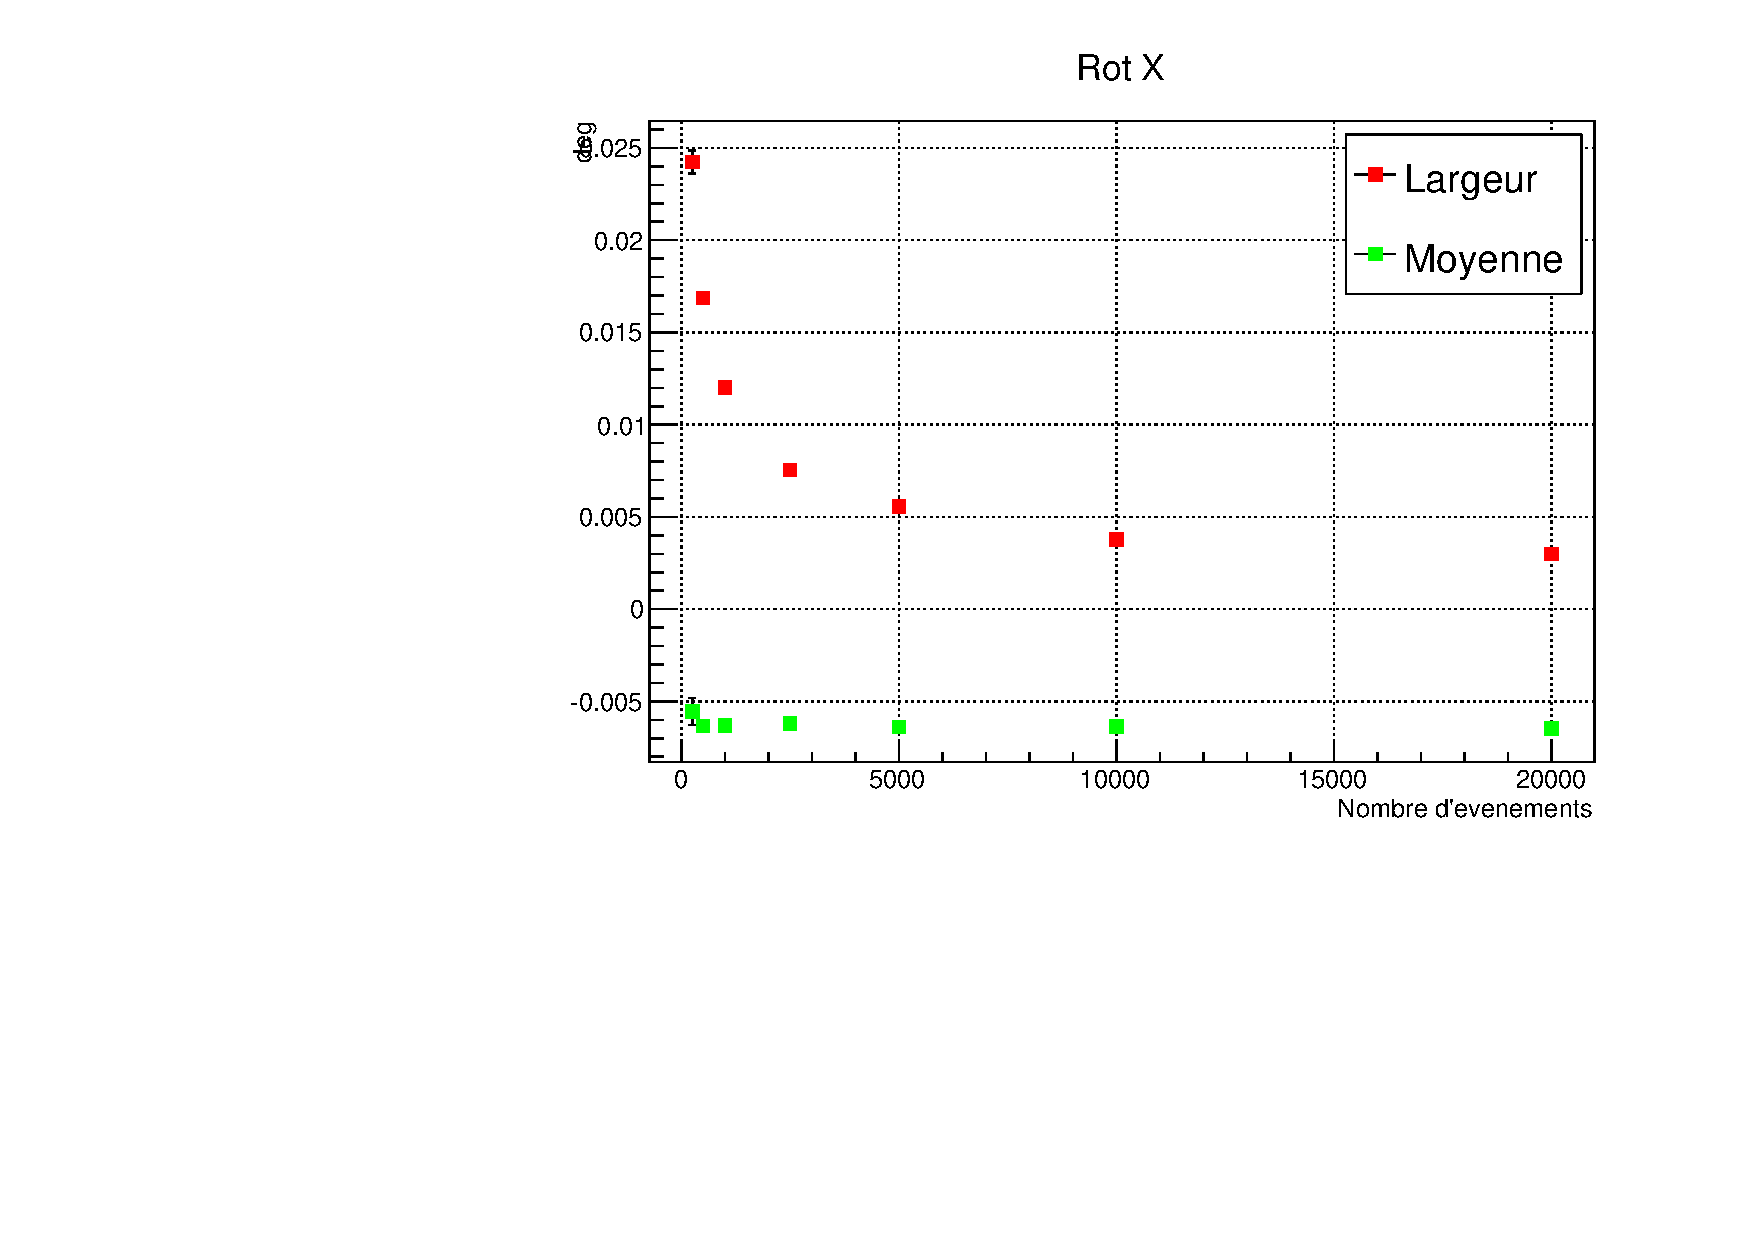
\includegraphics[width=0.78\textwidth]{./figures/Mini_Vexteurs_Alignement_Figures/precision_Rot_X.pdf}
%         }
%      \end{center}
%      \caption{Performances de la m\'ethode d'alignement avec mini-vecteur en fonction de la statistique utilis\'ee}
%      \label{fig:Precision_1}
%    \end{figure}
%    
%    \begin{figure}[htb!]
%      \begin{center}
%         \subfigure[En vert : \'ecart \`a la valeur Monte-Carlo de la valeur moyenne de la distribution du param\`etre $angleY$ apr\`es alignement, en fonction de la statistique. En rouge : largeur de la distribution du param\`etre $angleY$ apr\`es alignement, en fonction de la statistique.]{
%             \label{fig:MV_prec_Rot_Y}
%             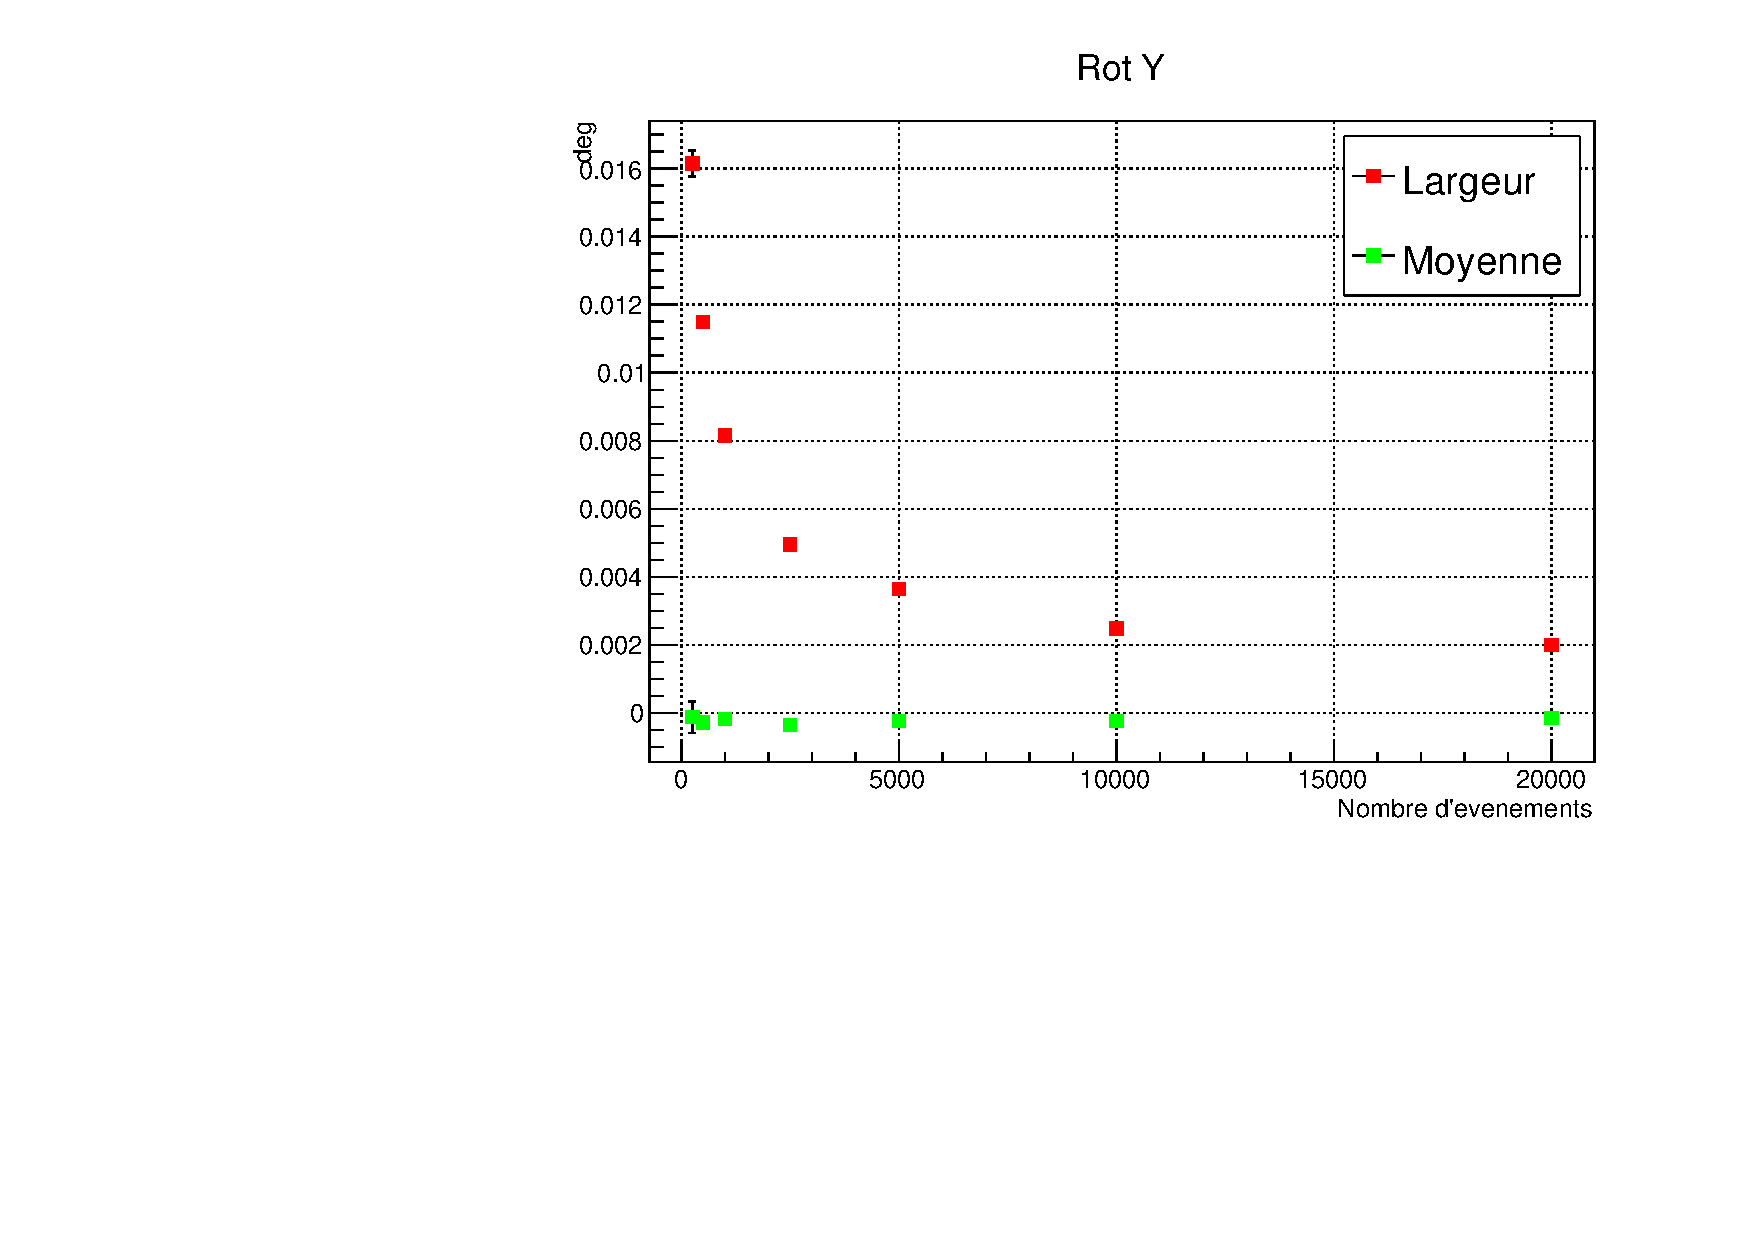
\includegraphics[width=0.78\textwidth]{./figures/Mini_Vexteurs_Alignement_Figures/precision_Rot_Y.pdf}
%         }
%         \subfigure[En vert : \'ecart \`a la valeur Monte-Carlo de la valeur moyenne de la distribution du param\`etre $angleZ$ apr\`es alignement, en fonction de la statistique. En rouge : largeur de la distribution du param\`etre $angleZ$ apr\`es alignement, en fonction de la statistique.]{
%            \label{fig:MV_prec_Rot_Z}
%            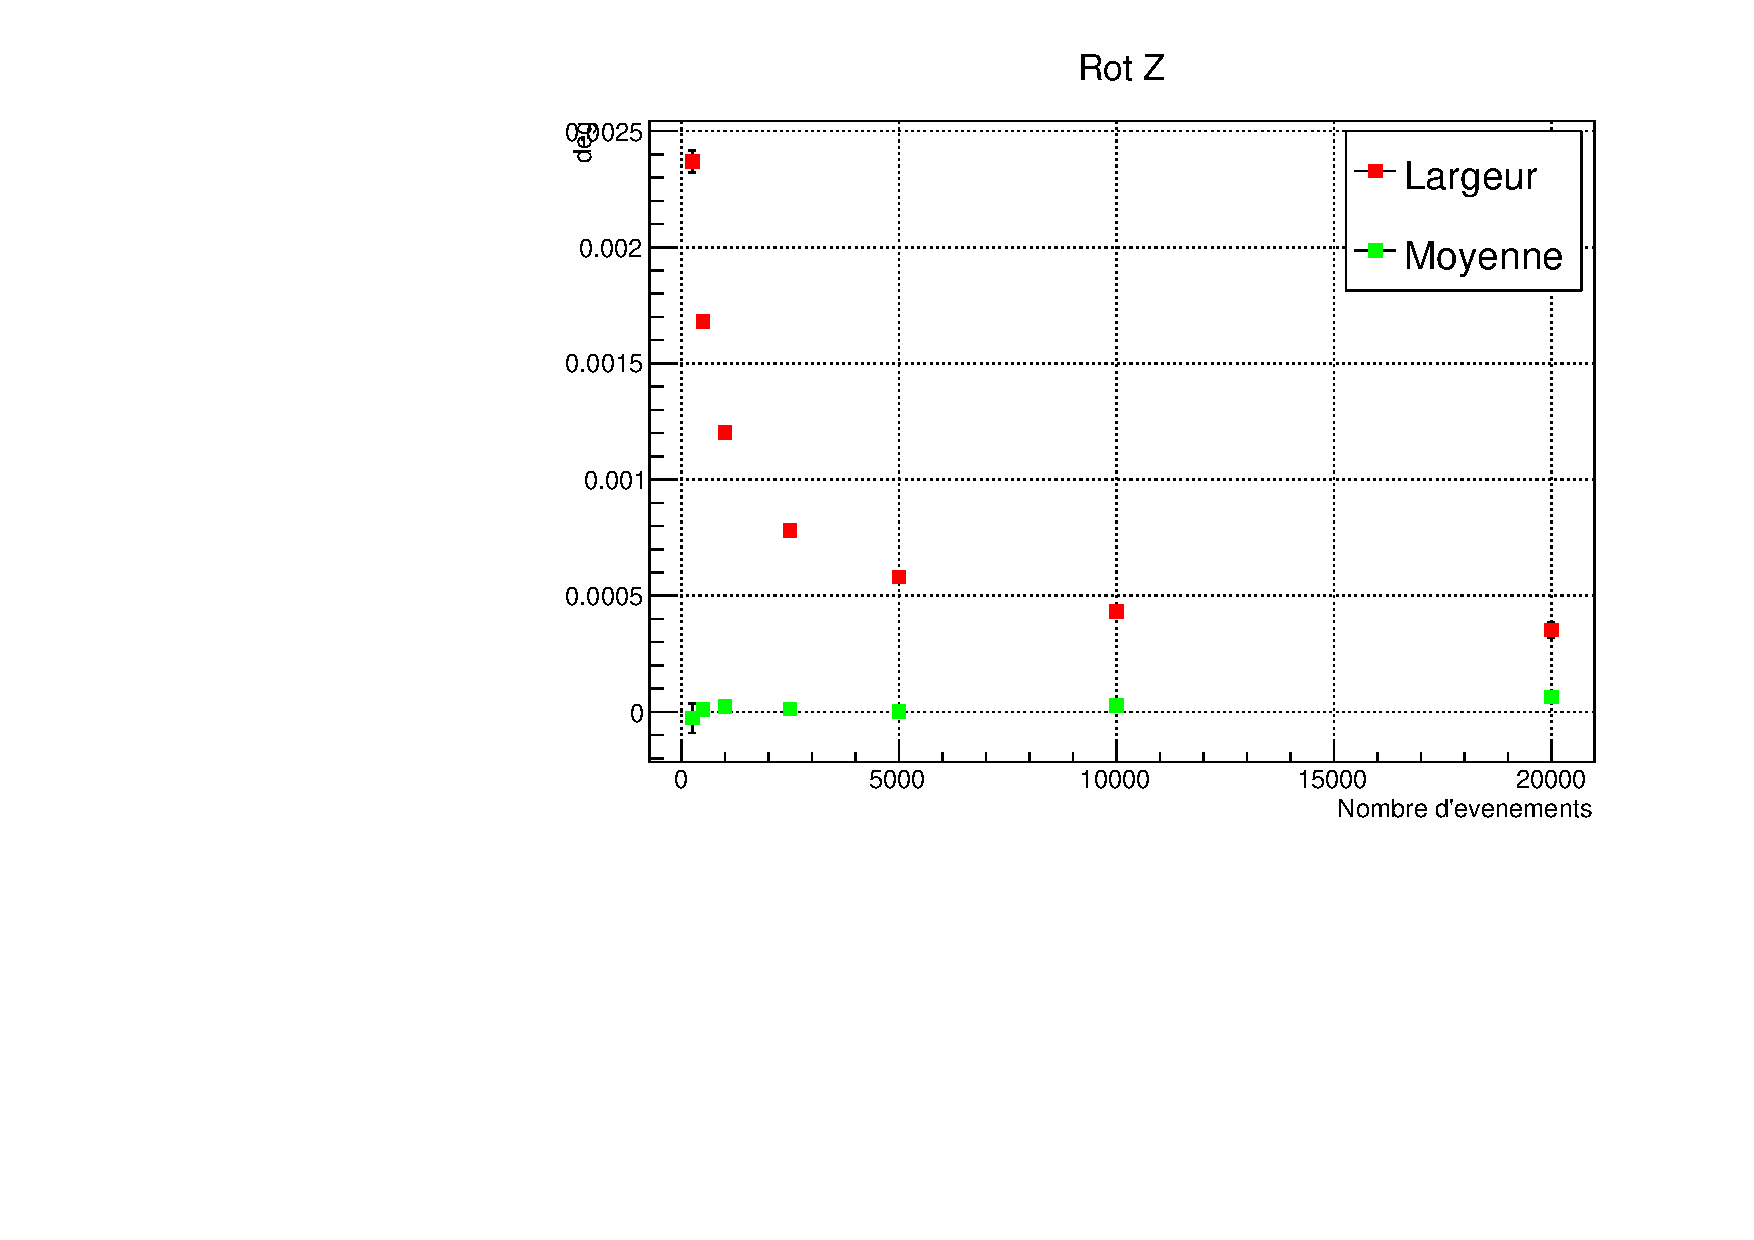
\includegraphics[width=0.78\textwidth]{./figures/Mini_Vexteurs_Alignement_Figures/precision_Rot_Z.pdf}
%         }
%      \end{center}
%      \caption{Performances de la m\'ethode d'alignement avec mini-vecteur en fonction de la statistique utilis\'ee}
%      \label{fig:Precision_2}
%    \end{figure}
%    
%    \FloatBarrier

%    On retiendra de cette \'etude que les param\`etres X1 et Y1 sont retrouv\'es avec une résolution inf\'erieur au microm\`etre \`a partir de 500 couples de mini-vecteurs bien associ\'es. Cette r\'esolution diminue \`a $0.2 \, \mu m$ avec 10 000 couples de mini-vecteurs bien align\'es. Pour les inclinaisons de l'\'echelle, celle-ci sont retrouv\'ees avec une pr\'ecision sup\'erieure \`a $2.5 \, 10^{-2}$ degr\'e. Cependant 
%    un biais sur la coordonn\'ee $Z1$ minimis\'ee existe. Ce biais est tr\`es certainement la r\'esultante d'un mode faible. Ainsi, pour retrouver la bonne valeur pour la coordonn\'ee $Z1$, il faut d\'efinir des contraintes sur ce param\`etre, ou utiliser des traces avec des inclinaisons diff\'erentes.
%    
%    \medskip
%    dire combien. 
%    \medskip
%    
%    Dur\'ee pour obtenir cette stat.
% 
% \chapter{Ajustement des vertex}
%   
%   L'objectif d'un d\'etecteur de vertex est d'identifier les vertex produits avec pr\'ecision afin d'identifier les saveurs des traces. Nous allons ici exposer une m\'ethode simple de reconstruction de vertex.
% 
%   \section{M\'ethode d'ajustement des vertex}
% 
%   Une fois l'alignement des diff\'erents d\'etecteurs composant l'exp\'erience effectu\'e, la recherche et l'ajustement des vertex peut alors d\'ebuter. La m\'ethode est la suivante : les traces sont d'abord reconstruites, puis, une fois les traces d\'ecouvertes et ajust\'ees, les vertex sont ajust\'es. Une m\'ethode simple bas\'ee sur la minimisation du $\chi^2$ est utilis\'ee.
% 
%   \medskip
% 
%   Pour calculer le $\chi^2$ on utilise la relation donnant la distance minimale d'approche d'un point \`a une droite. Soit $d_i$ la distance minimale d'approche d'un point M \`a une trace $\Delta_i$. La figure \ref{fig:dist_point_droite} pr\'esente le cas d'une droite et d'un point. Nous voulons calculer le cas ou il existe un nombre $N_t$ de traces et un vertex (point) M.
%   
%   \begin{figure}[htbp]
%    \begin{center}
%     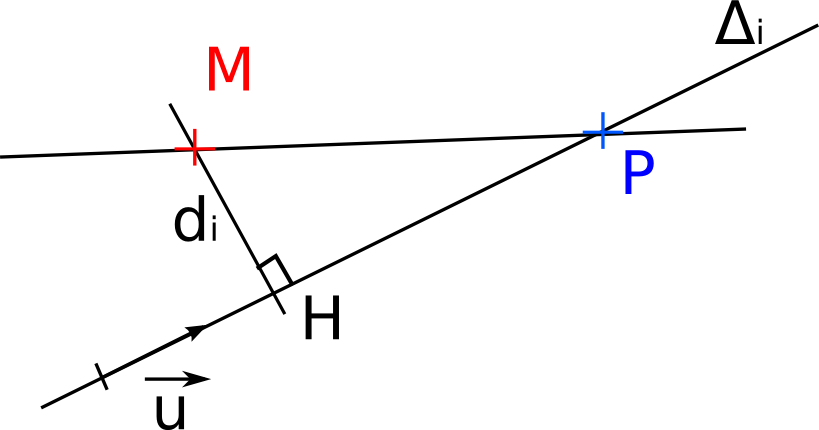
\includegraphics[scale=1.50]{./figures/Vertexing/schema_vertex.png}
%    \end{center}
%    \caption{Distance minimale d'approche d'un point M \`a une droite $\Delta_i$. L'objectif est la minimisation de la distance $d_i$. P est un point quelconque appartenant \`a la droite $d_i$.}
%    \label{fig:dist_point_droite}
%   \end{figure}
%   
%   \subsection{D\'etermination du $\chi^2$}
%   
%    Afin d'exprimer le $\chi^2$, nous allons calculer la distance minimale d'approche d'un point M aux droites $\Delta_i$. D'apr\`es la figure \ref{fig:dist_point_droite}, le th\'eor\`eme de Pythagore donne :
% 
%    \[ d_i^2 = PM^2 - \left( \vec{PM}.\vec{u_i} \right)^2 \]
% 
%    On pose dans le rep\`ere du laboratoire  : les coordonn\'ees du point $P(x_p, y_p, z_p)$ appartenant \`a la trace consid\'er\'ee, les coordonn\'ees du vertex $M(x_i, y_i, z_i)$ et les composantes normalis\'ees du vecteur directeur de la trace $\vec{u_i} = (u_x, u_y, u_z)$. La distance minimale d'approche s'exprime alors de la fa\c{c}on suivante :
%    
%    \[ d_i^2 = (x_i-x_p)^2 + (y_i-y_p)^2 + (z_i-z_p)^2 - \left( (x_i-x_p) u_x + (y_i-y_p) u_y + (z_i-z_p) u_z \right)^2  \]
% 
%    Le $\chi^2$ est d\'efini par :
% 
%    \[  \chi^2 = \sum_{traces} \sum_i \cfrac{d_i^2}{\sigma_i^2} \]
%    
%    Avec $\sigma_i$ les erreurs sur les distances $d_i$ (distances minimales trace-vertex) provenant des erreurs possibles sur la droite $d_i$. On calcule les termes $\sigma_i$ gr\^ace \`a une relation de propagation des erreurs. On a alors : 
% 
%    \[ \sigma_i^2 = \left( \cfrac{\partial d_i}{\partial x_i} \right)^2 {\sigma_{x_i}}^2 + \left( \cfrac{\partial d_i}{\partial y_i} \right)^2 {\sigma_{y_i}}^2 + \left( \cfrac{\partial d_i}{\partial z_i} \right)^2 {\sigma_{z_i}}^2 \]
% 
%    Soit :
% 
%    \[ \cfrac{\partial d_i}{\partial x_i} = \cfrac{ (1-u_x^2)(x_i-x_p) - 2 (y_i-y_p)u_y u_x - 2 (z_i-z_p) u_x u_z }{2 d_i} \]
% 
%    \[ \cfrac{\partial d_i}{\partial y_i} = \cfrac{ (1-u_y^2)(y_i-y_p) - 2 (x_i-x_p)u_y u_x - 2 (z_i-z_p) u_y u_z }{2 d_i} \]
% 
%    \[ \cfrac{\partial d_i}{\partial z_i} = \cfrac{ (1-u_z^2)(z_i-z_p) - 2 (x_i-x_p)u_z u_x - 2 (y_i-y_p) u_y u_z }{2 d_i} \]
% 
%    
%    Les $\sigma_i$ valent donc : 
%    
%    \[ \sigma_i^2 = \left( \cfrac{ (1-u_x^2)(x_i-x_p) - 2 (y_i-y_p)u_y u_x - 2 (z_i-z_p) u_x u_z }{2 d_i} \right)^2 \sigma_{x_i}^2 \]
%    \[ + \left( \cfrac{ (1-u_y^2)(y_i-y_p) - 2 (x_i-x_p)u_y u_x - 2 (z_i-z_p) u_y u_z }{2 d_i} \right)^2 \sigma_{y_i}^2  \] 
%    \[ + \left( \cfrac{ (1-u_z^2)(z_i-z_p) - 2 (x_i-x_p)u_z u_x - 2 (y_i-y_p) u_y u_z }{2 d_i} \right)^2 \sigma_{z_i}^2 \]
%    
%    La minimisation du $\chi^2$ donne alors la position du vertex M reconstruit.
  
%   \section{R\'esultats}
% 
%    Afin de tester la m\'ethode, quelques graphiques de vertex simples avec un nombre $N_t$ de traces par \'ev\'enements ont \'et\'e r\'ealis\'es.
%    Des \'etudes plus pouss\'ees n'ont pas \'et\'e effectu\'ees.
% 
% \chapter{Resultats Taux d'occupation}
% \label{resultats_tx_occupation}

\chapter{Bruit de fond faisceau}

\section{Angles d'incidence du bruit de fond :}
\label{annexe:angles_incidence}
  
  \begin{figure}[!htb]
    \centering
    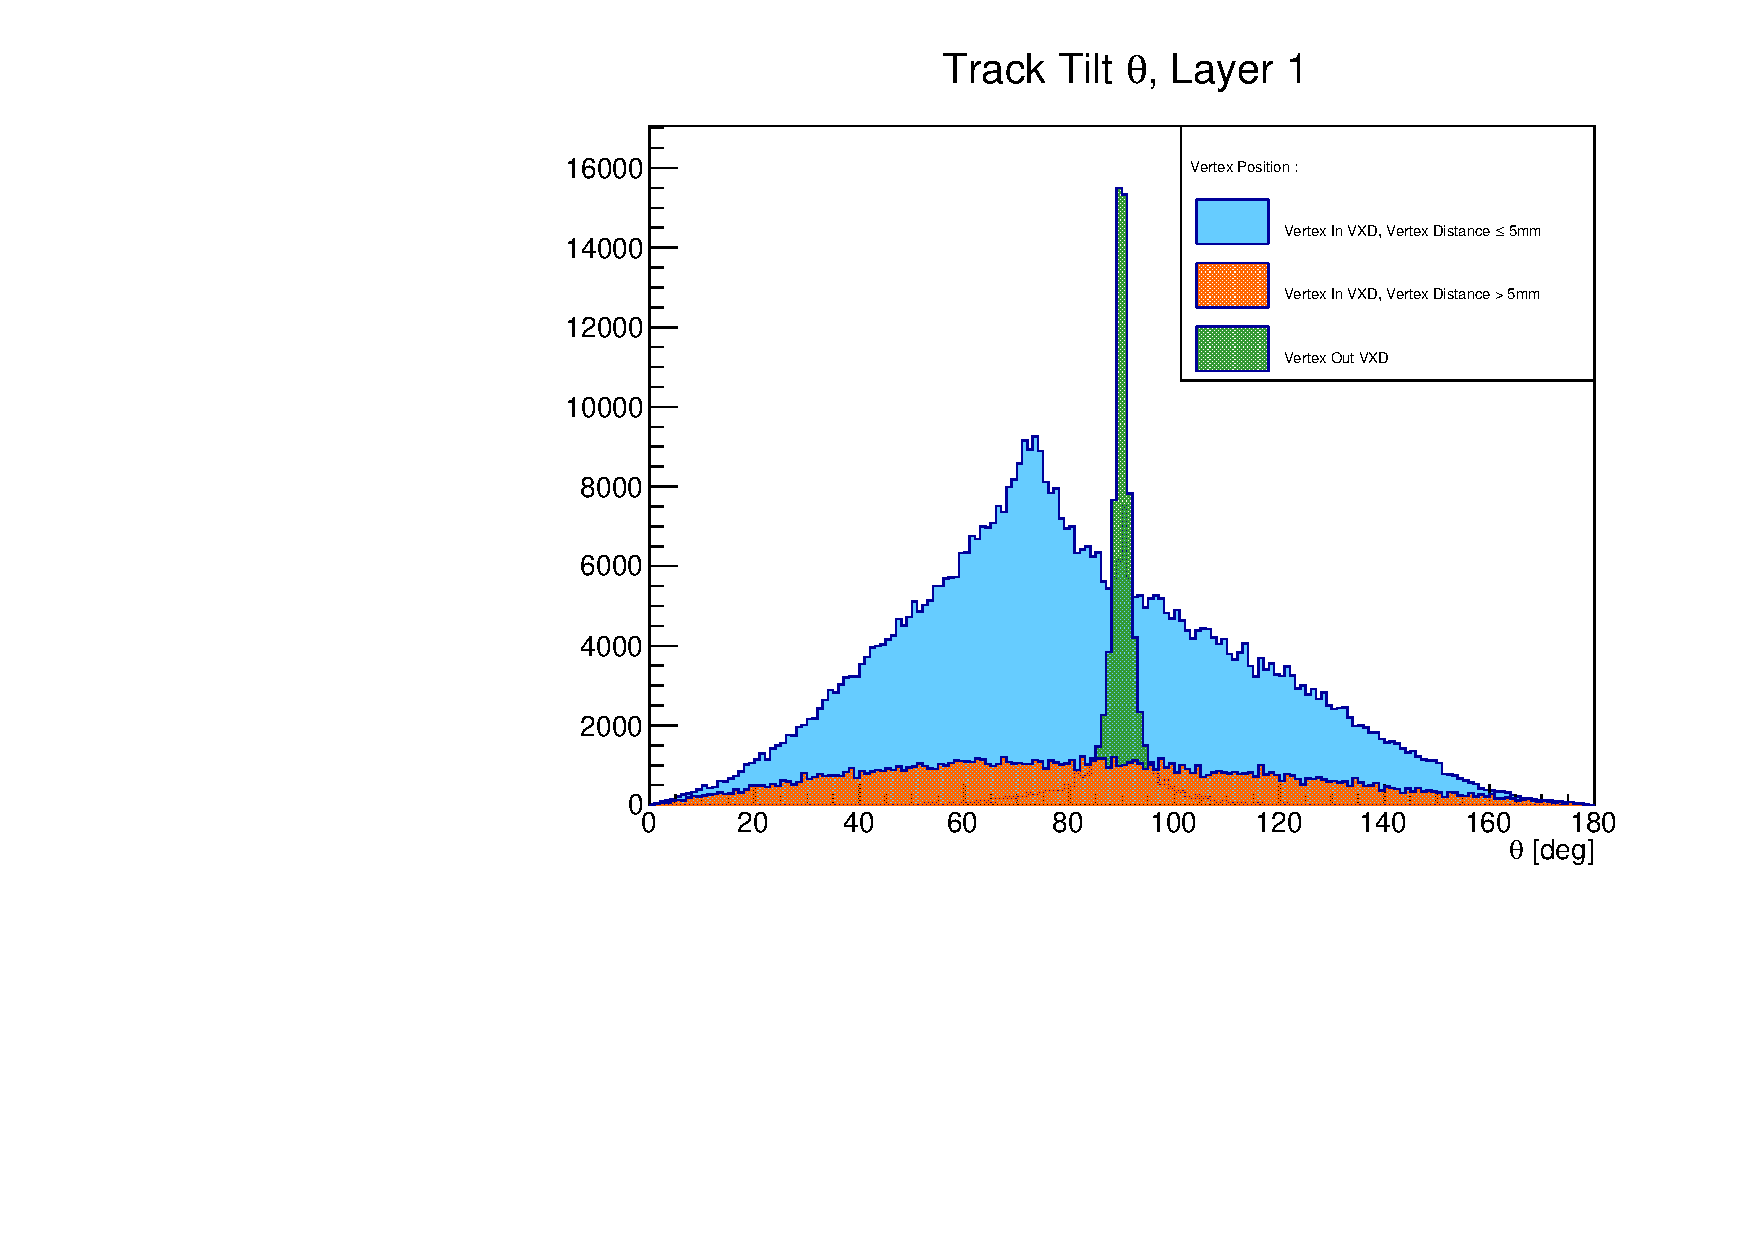
\includegraphics[scale=0.58]{./figures/Track_Tilts_Beamstrahlung/beamstrahlung_Theta/Track_Tilts_Theta_Layer1.pdf}
    \caption{Distribution des angles $\theta$ reconstruits pour chaque impact sur les \'echelles de la couche 1. Les couleurs bleue, rouge et verte distinguent les positions des vertex des particules associ\'ees aux impacts.}
    \label{fig:theta_Layer1}
  \end{figure}  
    
  \begin{figure}[!htb]
    \centering
    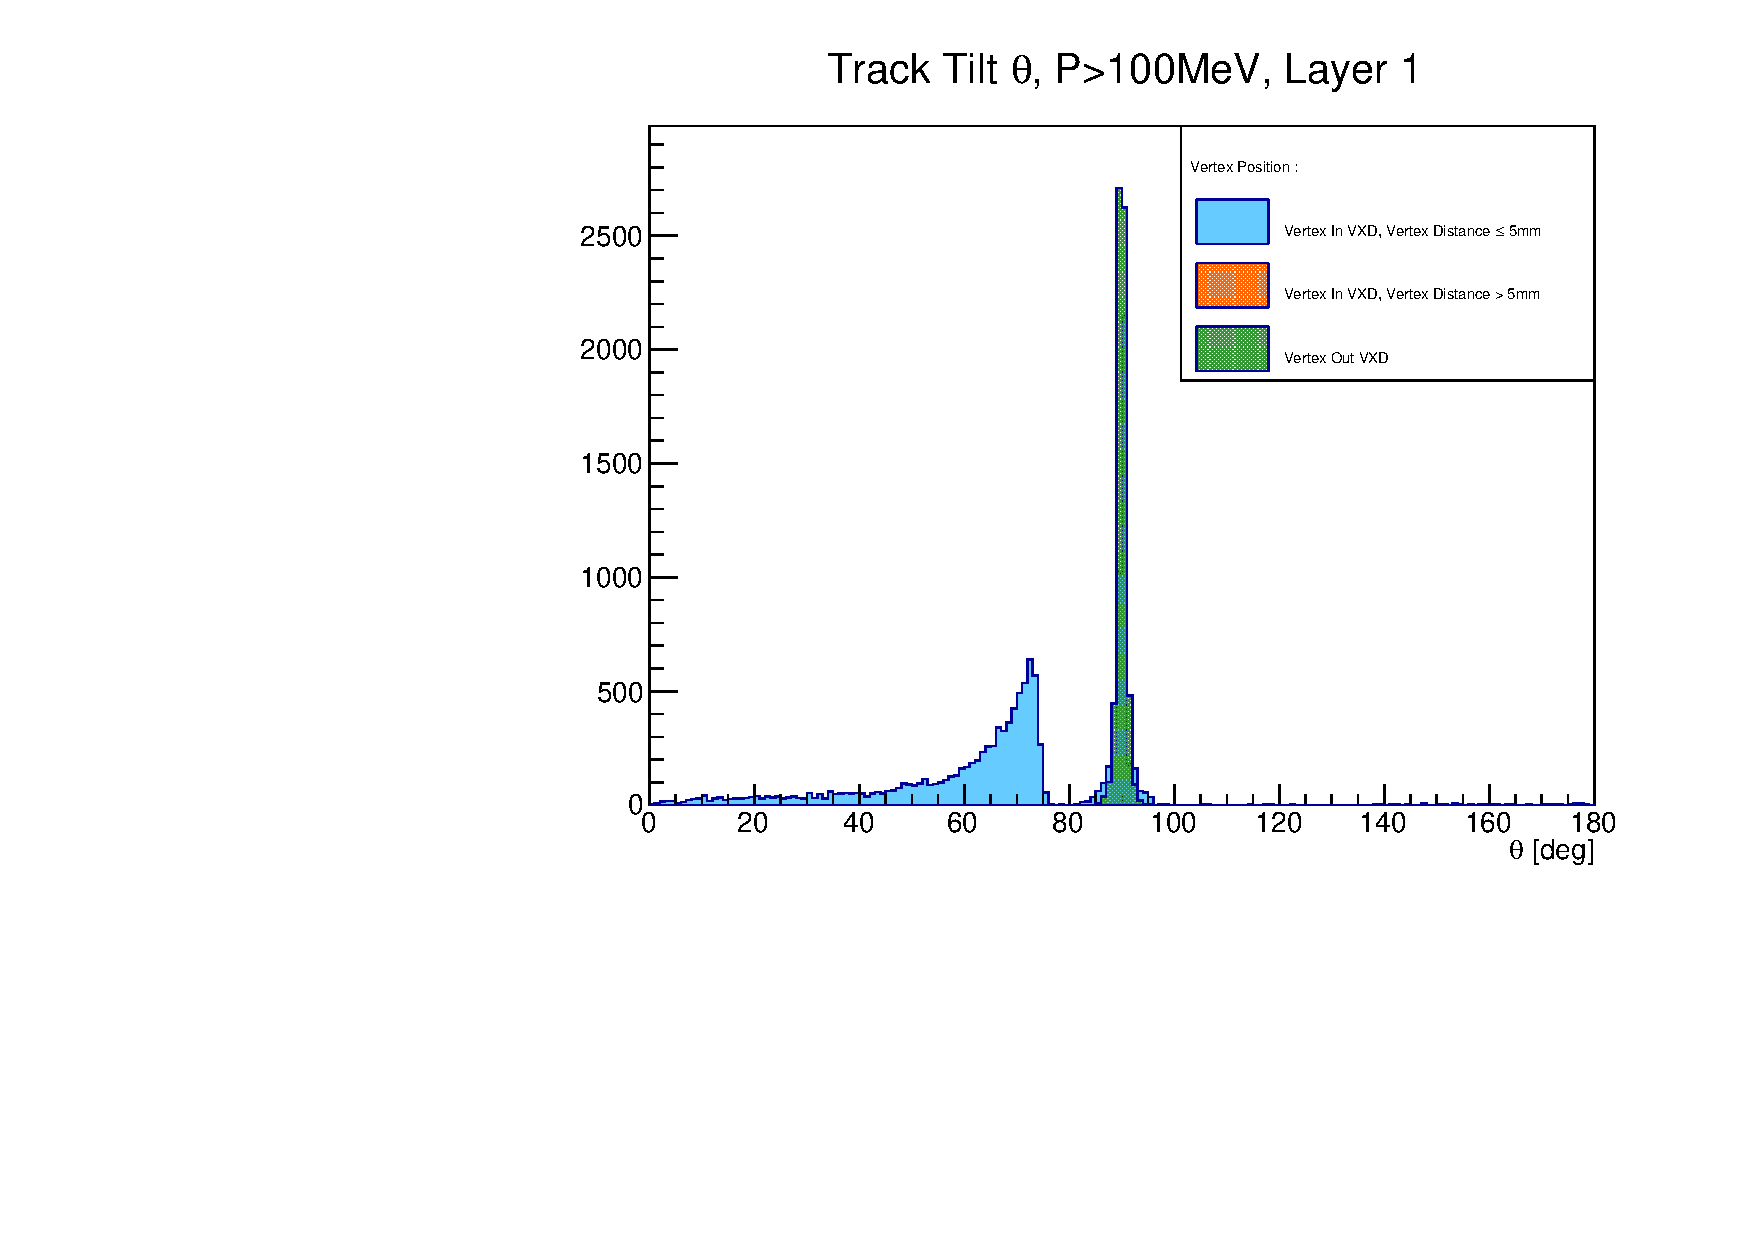
\includegraphics[scale=0.58]{./figures/Track_Tilts_Beamstrahlung/beamstrahlung_Theta/Track_Tilts_Theta_P_sup_100MeV_Layer1.pdf}
    \caption{Angle d'incidence $\theta$ associ\'e aux impacts de bruit de fond d'impulsion sup\'erieure \`a $100 MeV/c$ de la couche 1 en fonction de la position des impacts selon l'axe $U$ de l'\'echelle consid\'er\'ee.}
    \label{fig:theta_Layer1_pT_sup_100MeV}
  \end{figure}
  
  \begin{figure}[!htb]
    \centering
    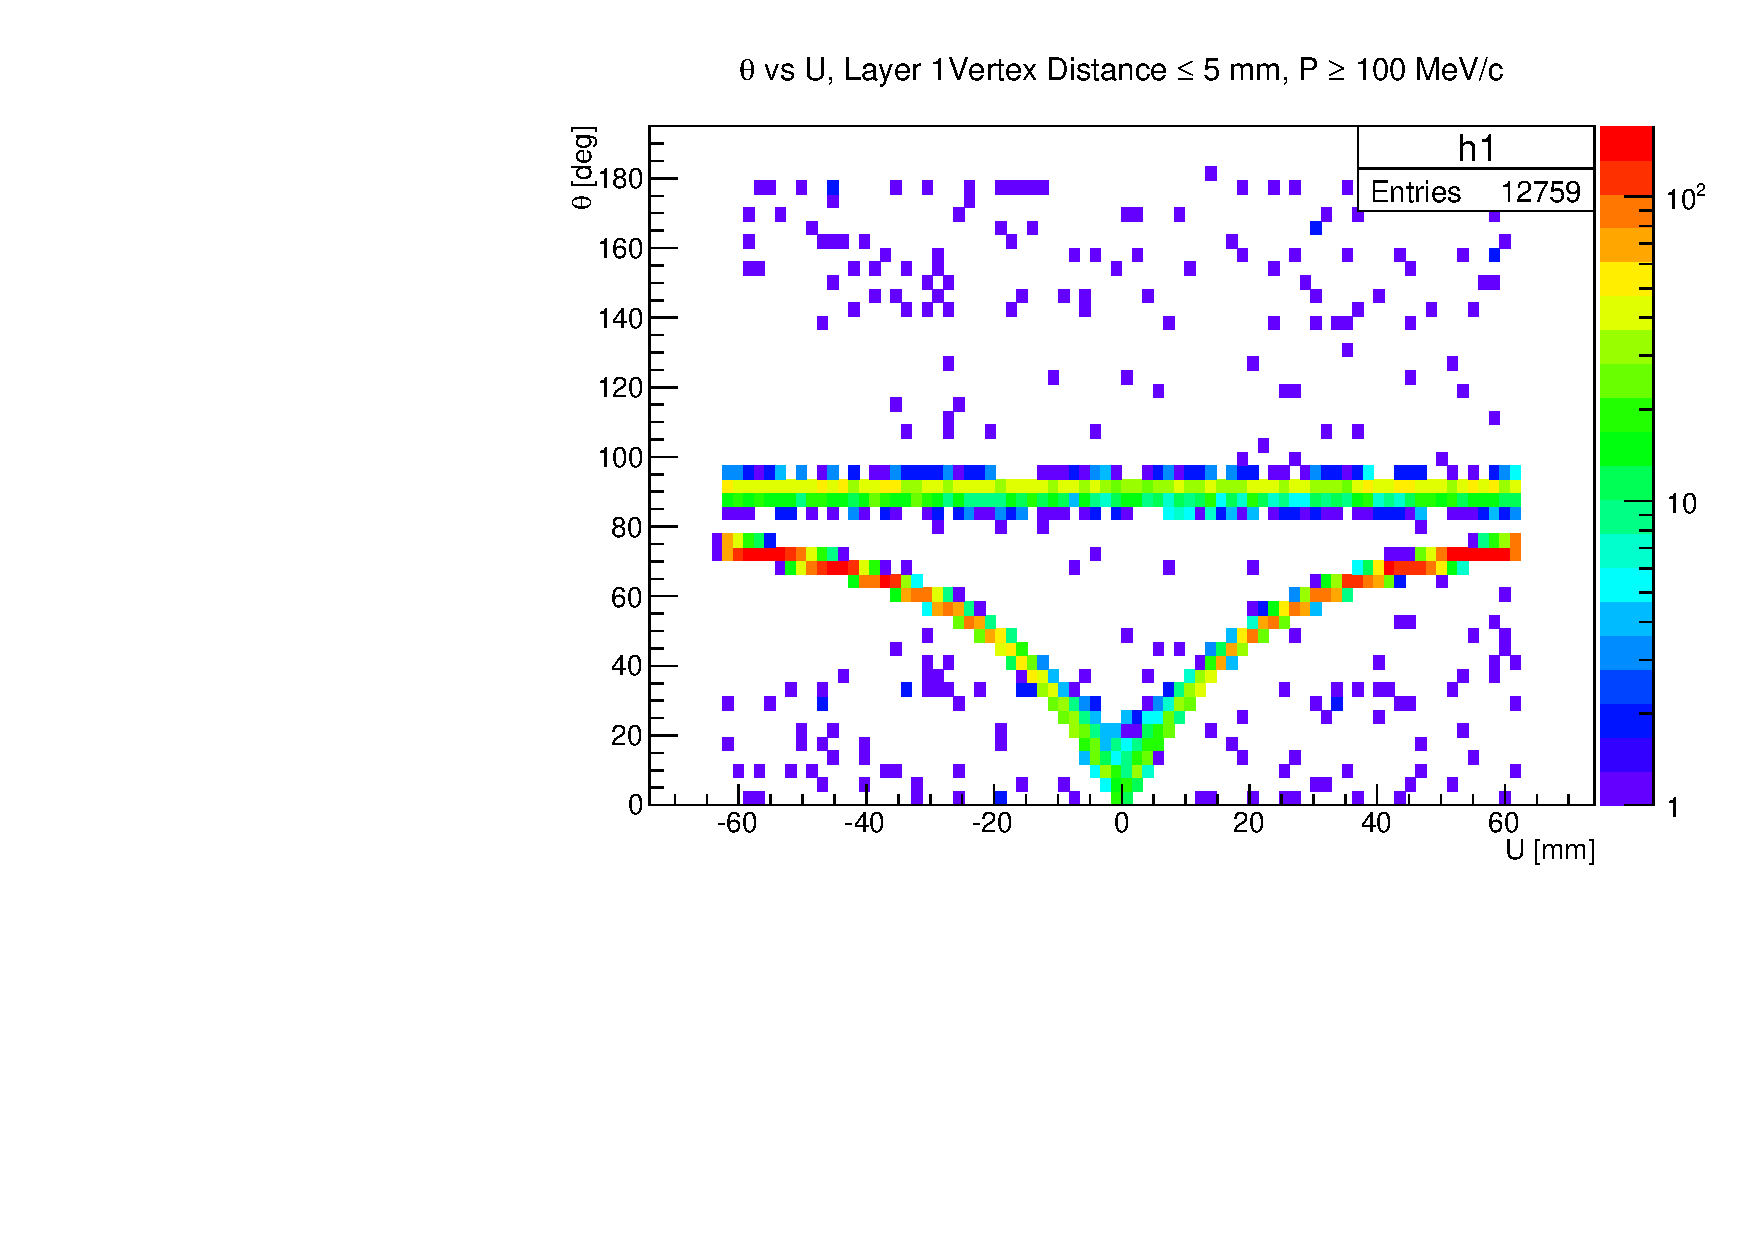
\includegraphics[scale=0.58]{./figures/Track_Tilts_Beamstrahlung/beamstrahlung_Theta/Track_Tilts_Theta_vs_U_P_sup_100MeV_vertex_inf_5mm_Layer1.pdf}
    \caption{Angle local $\phi$ associ\'e \`a chaque impact de bruit de fond de la couche 1 en fonction de la position de l'impact selon l'axe $U$ de l'\'echelle. Seuls les impacts dont le vertex de la particule correspondante est situ\'ee dans une sph\`ere de 5 $mm$ autour du point d'interaction sont trac\'es.}
    \label{fig:theta_Layer1_vs_U_P_sup_100MeV_vertex_inf_5mm}
  \end{figure}
  
  \begin{figure}[!htb]
    \centering
    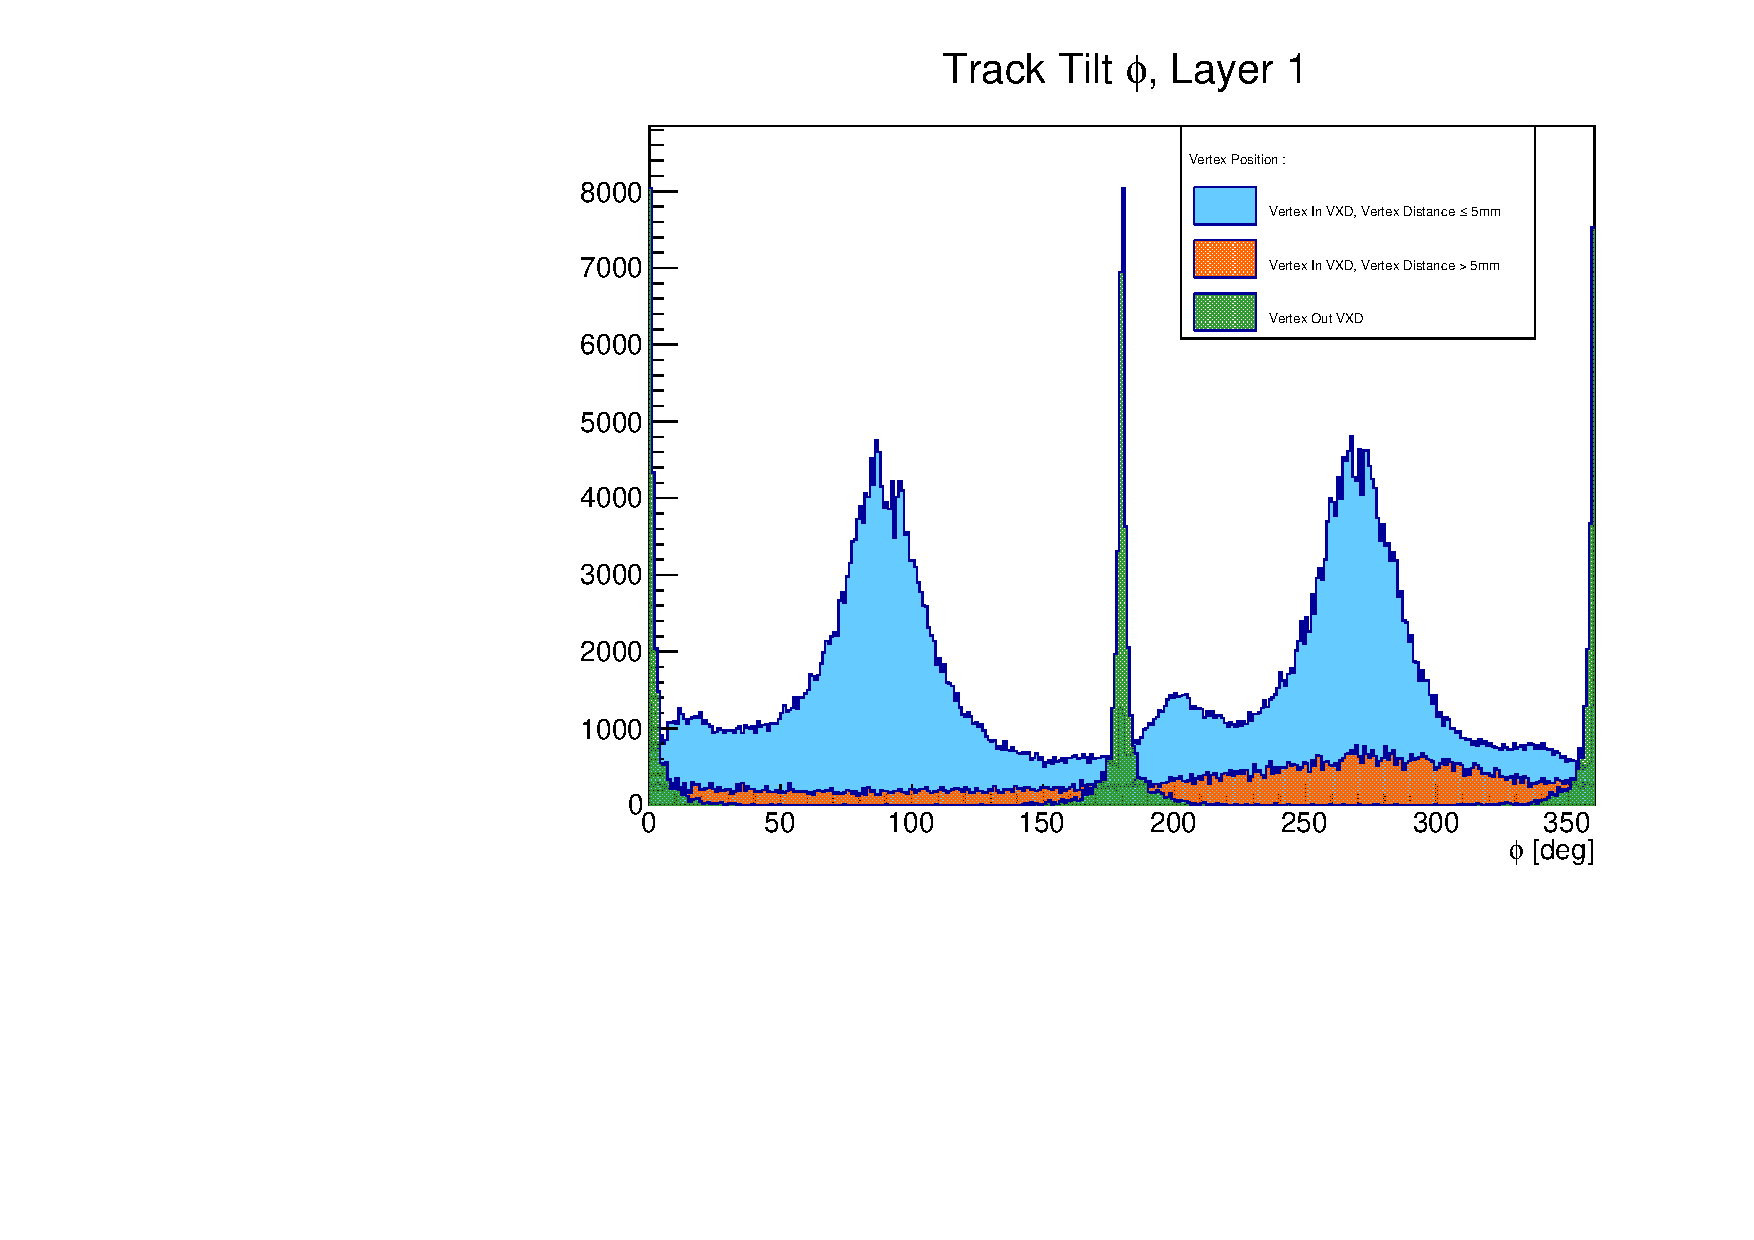
\includegraphics[scale=0.58]{./figures/Track_Tilts_Beamstrahlung/beamstrahlung_Phi/Track_Tilts_Phi_Layer1.pdf}
    \caption{Angle local $\phi$ associ\'e \`a chaque impact de bruit de fond de la couche 1.}
    \label{fig:phi_Layer1}
  \end{figure}  
  
  \begin{figure}[!htb]
    \centering
    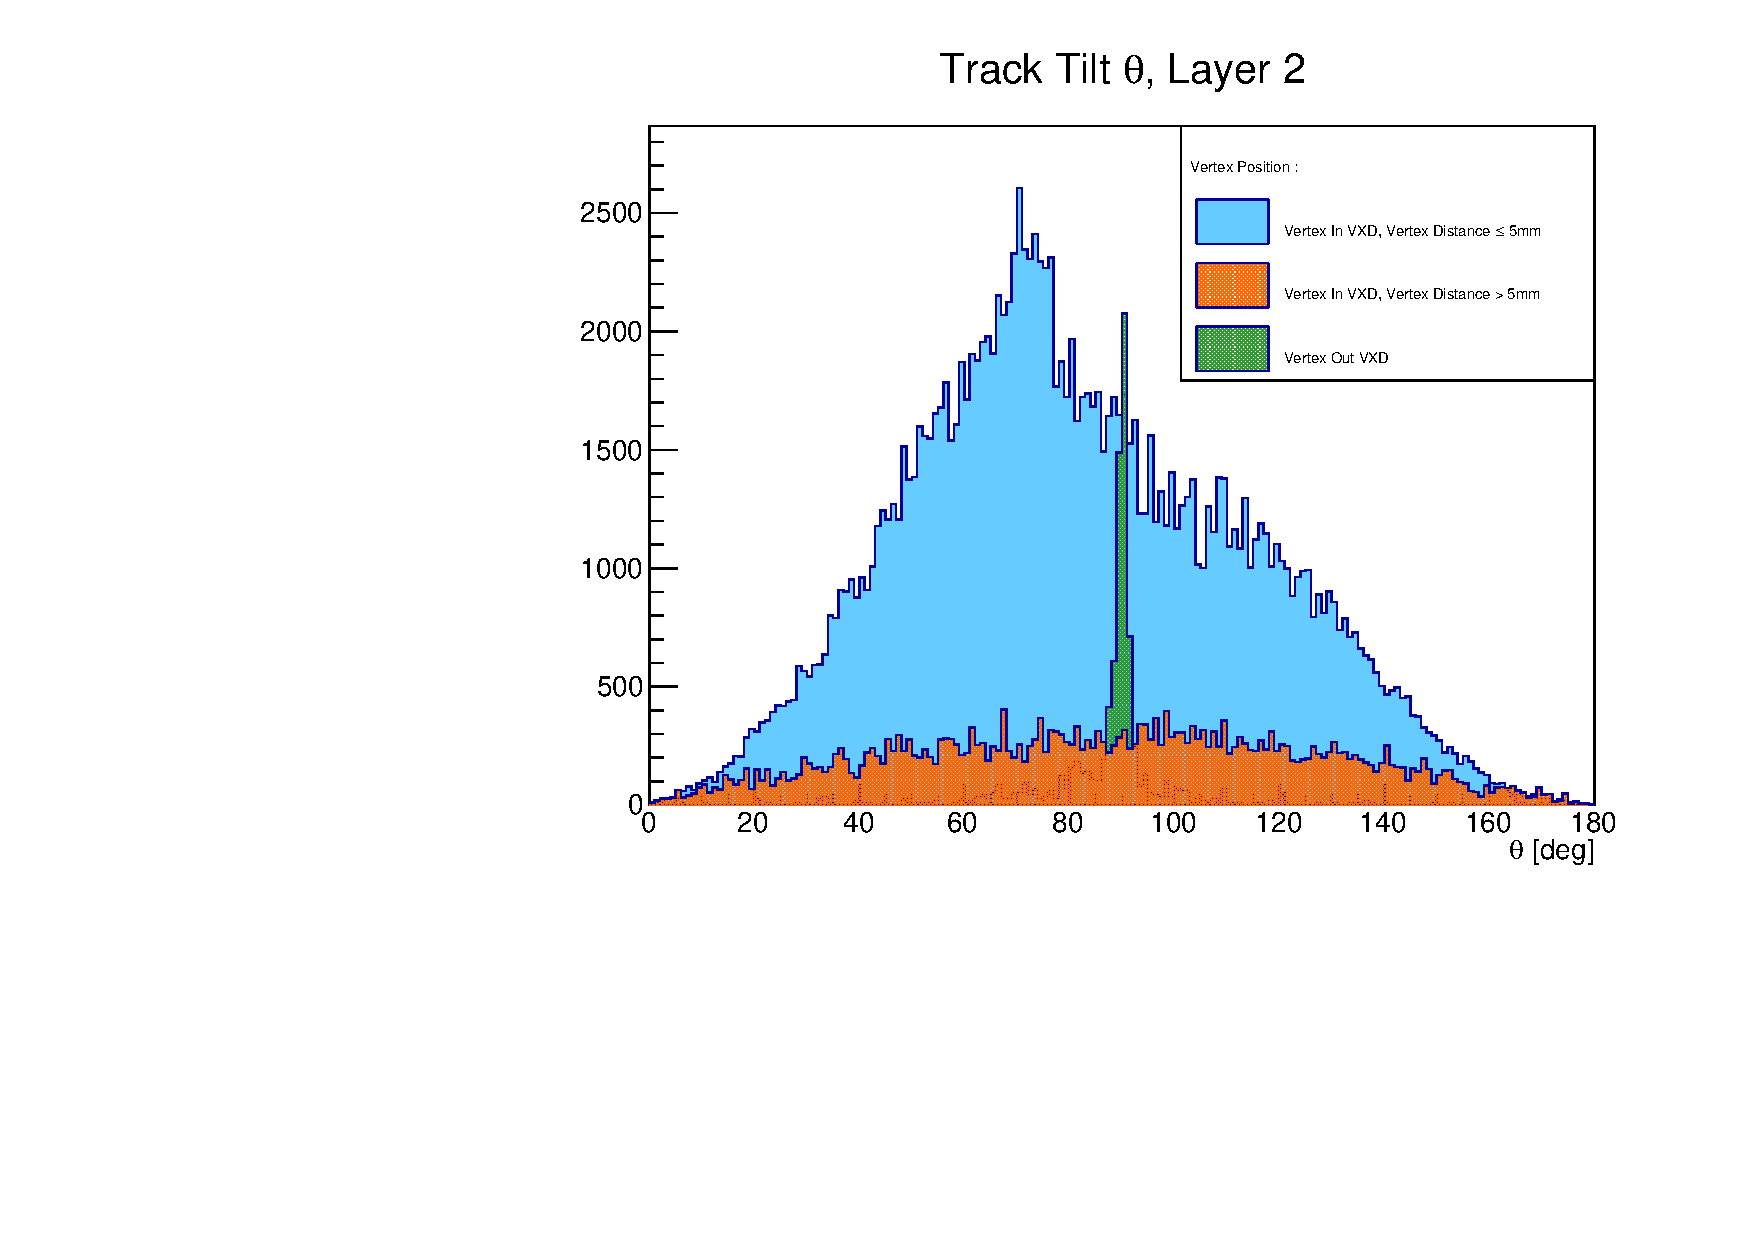
\includegraphics[scale=0.58]{./figures/Track_Tilts_Beamstrahlung/beamstrahlung_Theta/Track_Tilts_Theta_Layer2.pdf}
    \caption{Distribution des angles $\theta$ reconstruits pour chaque impact sur les \'echelles de la couche 2. Les couleurs bleue, rouge et verte distinguent les positions des vertex des particules associ\'ees aux impacts.}
    \label{fig:theta_Layer2}
  \end{figure}
  
  \begin{figure}[!htb]
    \centering
    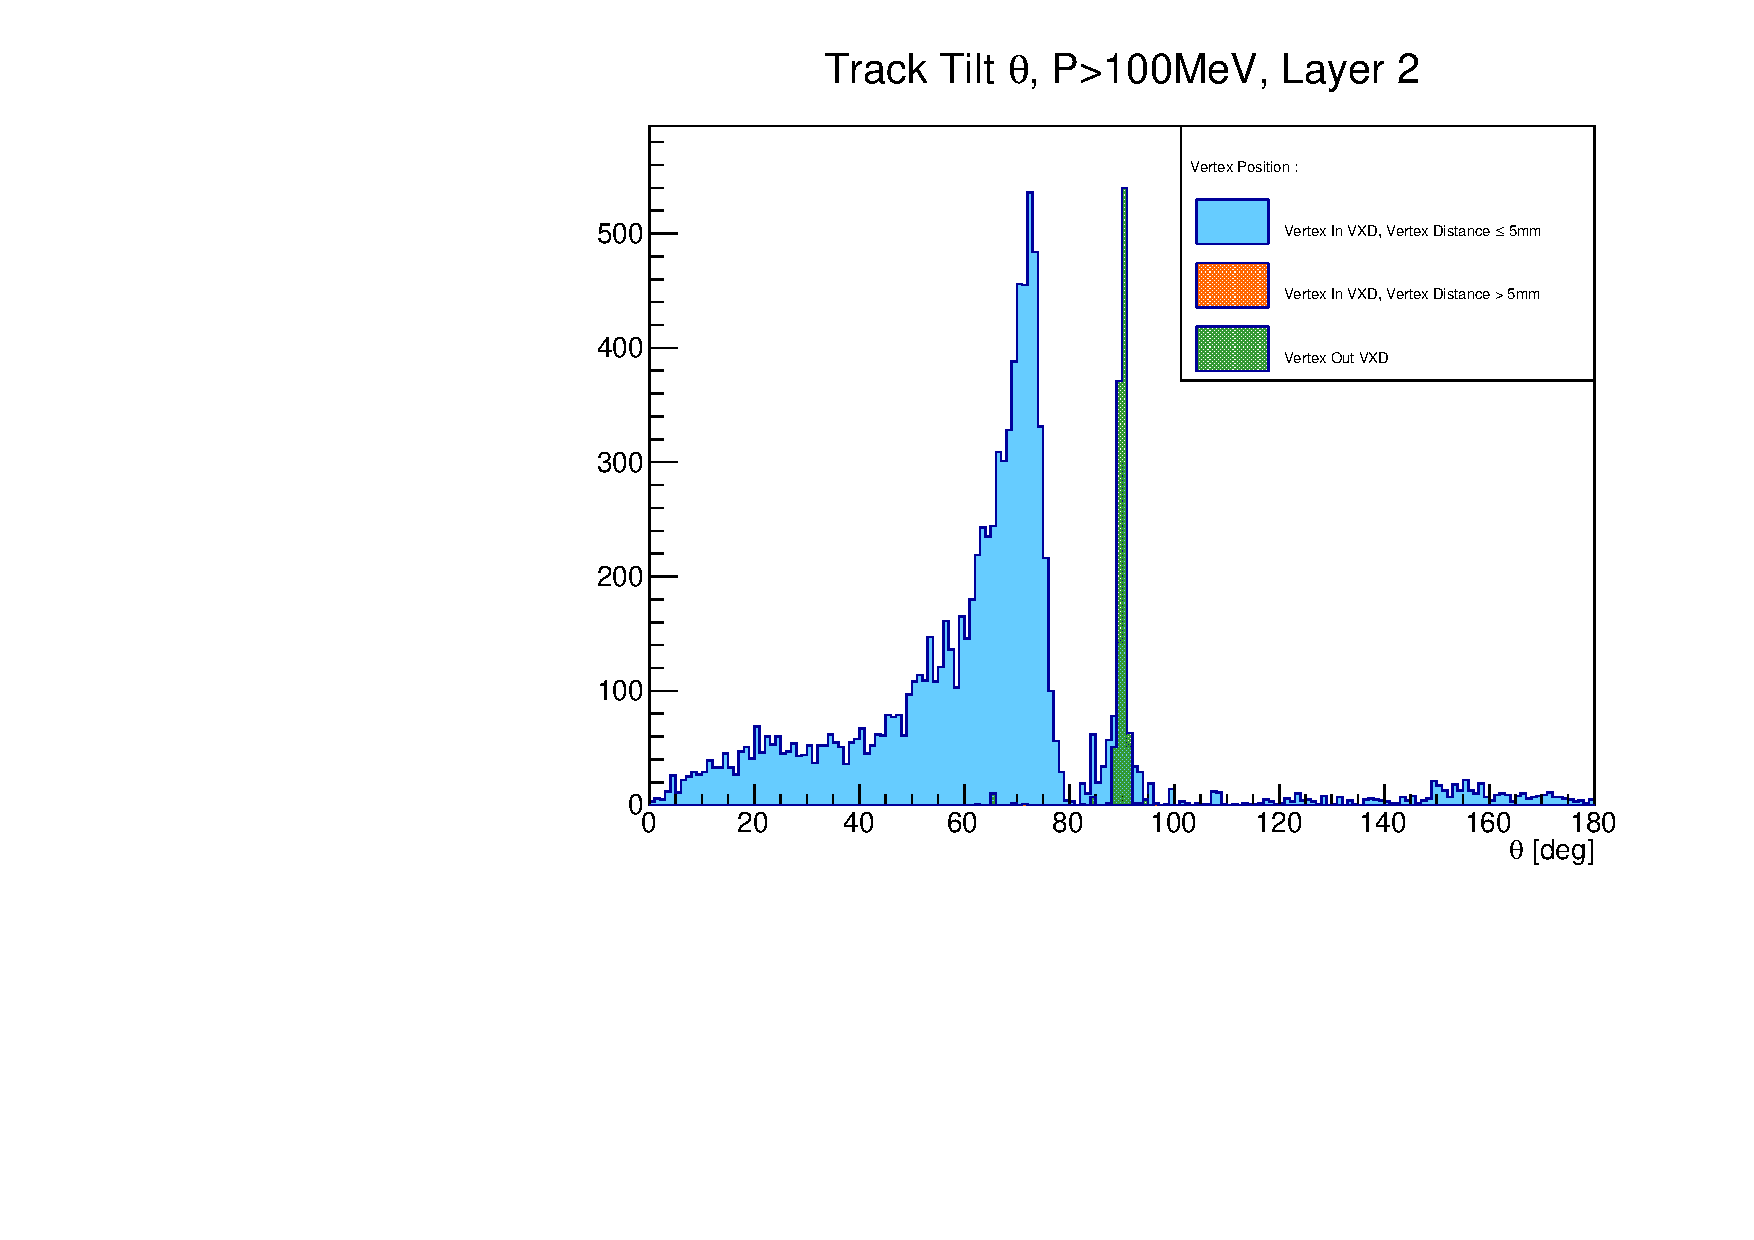
\includegraphics[scale=0.58]{./figures/Track_Tilts_Beamstrahlung/beamstrahlung_Theta/Track_Tilts_Theta_P_sup_100MeV_Layer2.pdf}
    \caption{Angle d'incidence $\theta$ associ\'e aux impacts de bruit de fond d'impulsion sup\'erieure \`a $100 MeV/c$ de la couche 2 en fonction de la position des impacts selon l'axe $U$ de l'\'echelle consid\'er\'ee.}
    \label{fig:theta_Layer2_pT_sup_100MeV}
  \end{figure}
  
  \begin{figure}[!htb]
    \centering
    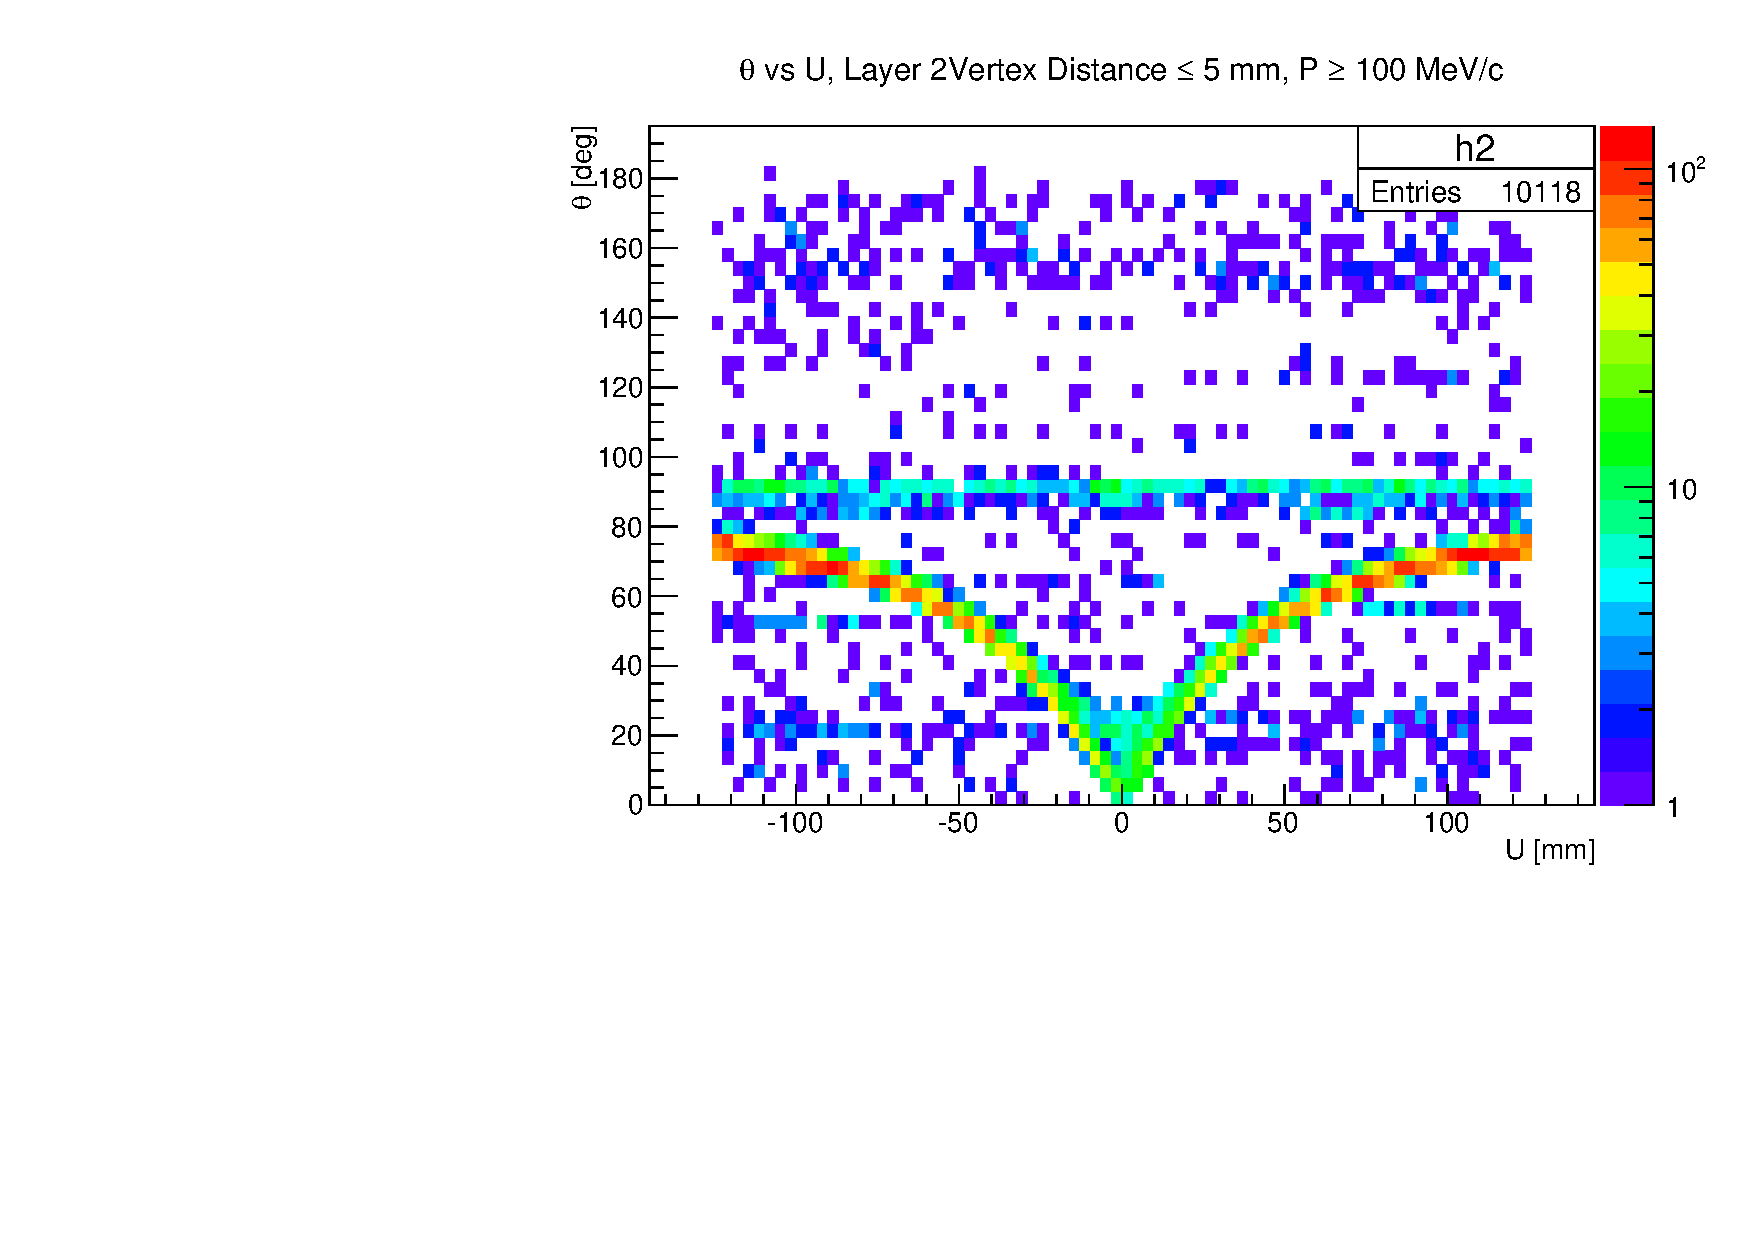
\includegraphics[scale=0.58]{./figures/Track_Tilts_Beamstrahlung/beamstrahlung_Theta/Track_Tilts_Theta_vs_U_P_sup_100MeV_vertex_inf_5mm_Layer2.pdf}
    \caption{Angle local $\phi$ associ\'e \`a chaque impact de bruit de fond de la couche 2 en fonction de la position de l'impact selon l'axe $U$ de l'\'echelle. Seuls les impacts dont le vertex de la particule correspondante est situ\'ee dans une sph\`ere de 5 $mm$ autour du point d'interaction sont trac\'es.}
    \label{fig:theta_Layer2_vs_U_P_sup_100MeV_vertex_inf_5mm}
  \end{figure}
  
  \begin{figure}[!htb]
    \centering
    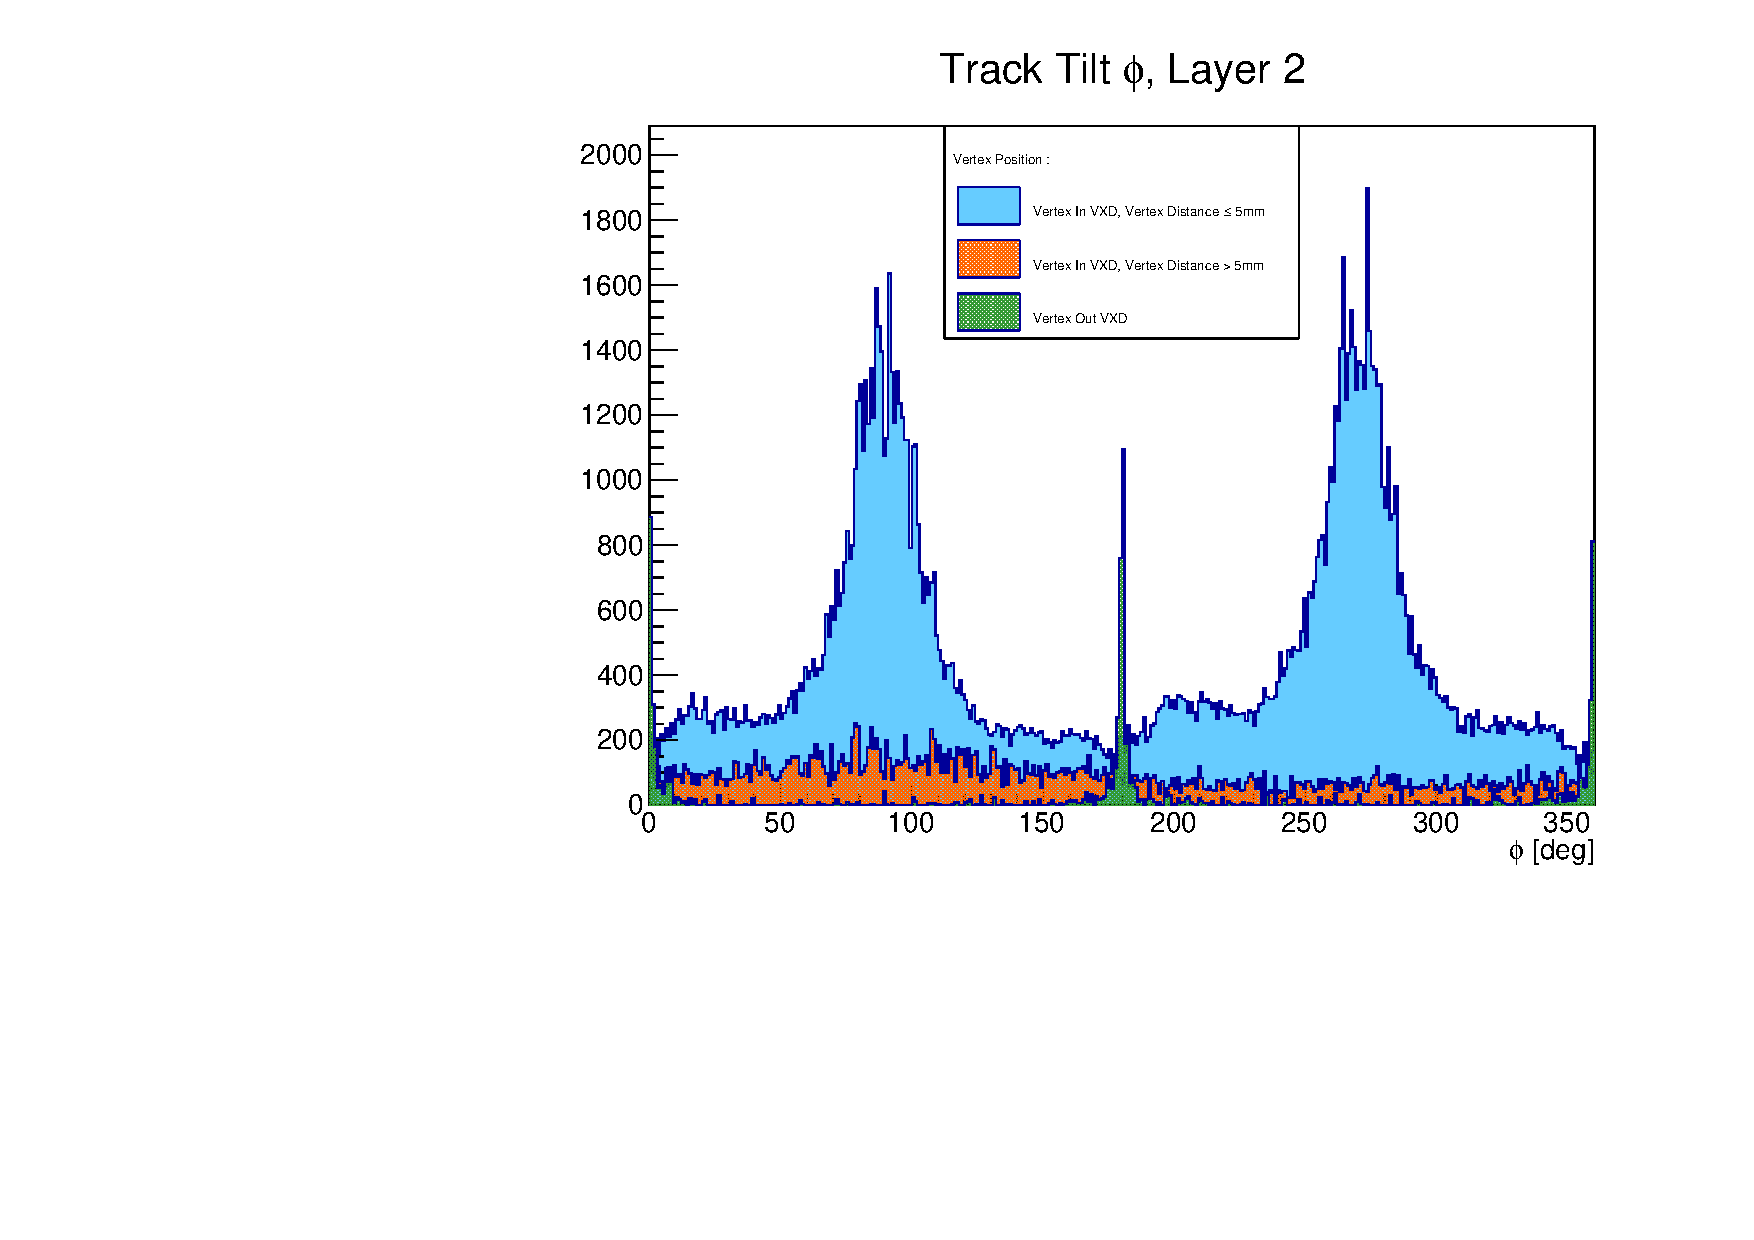
\includegraphics[scale=0.58]{./figures/Track_Tilts_Beamstrahlung/beamstrahlung_Phi/Track_Tilts_Phi_Layer2.pdf}
    \caption{Angle local $\phi$ associ\'e \`a chaque impact de bruit de fond de la couche 2.}
    \label{fig:phi_Layer2}
  \end{figure}
  
  \begin{figure}[!htb]
    \centering
    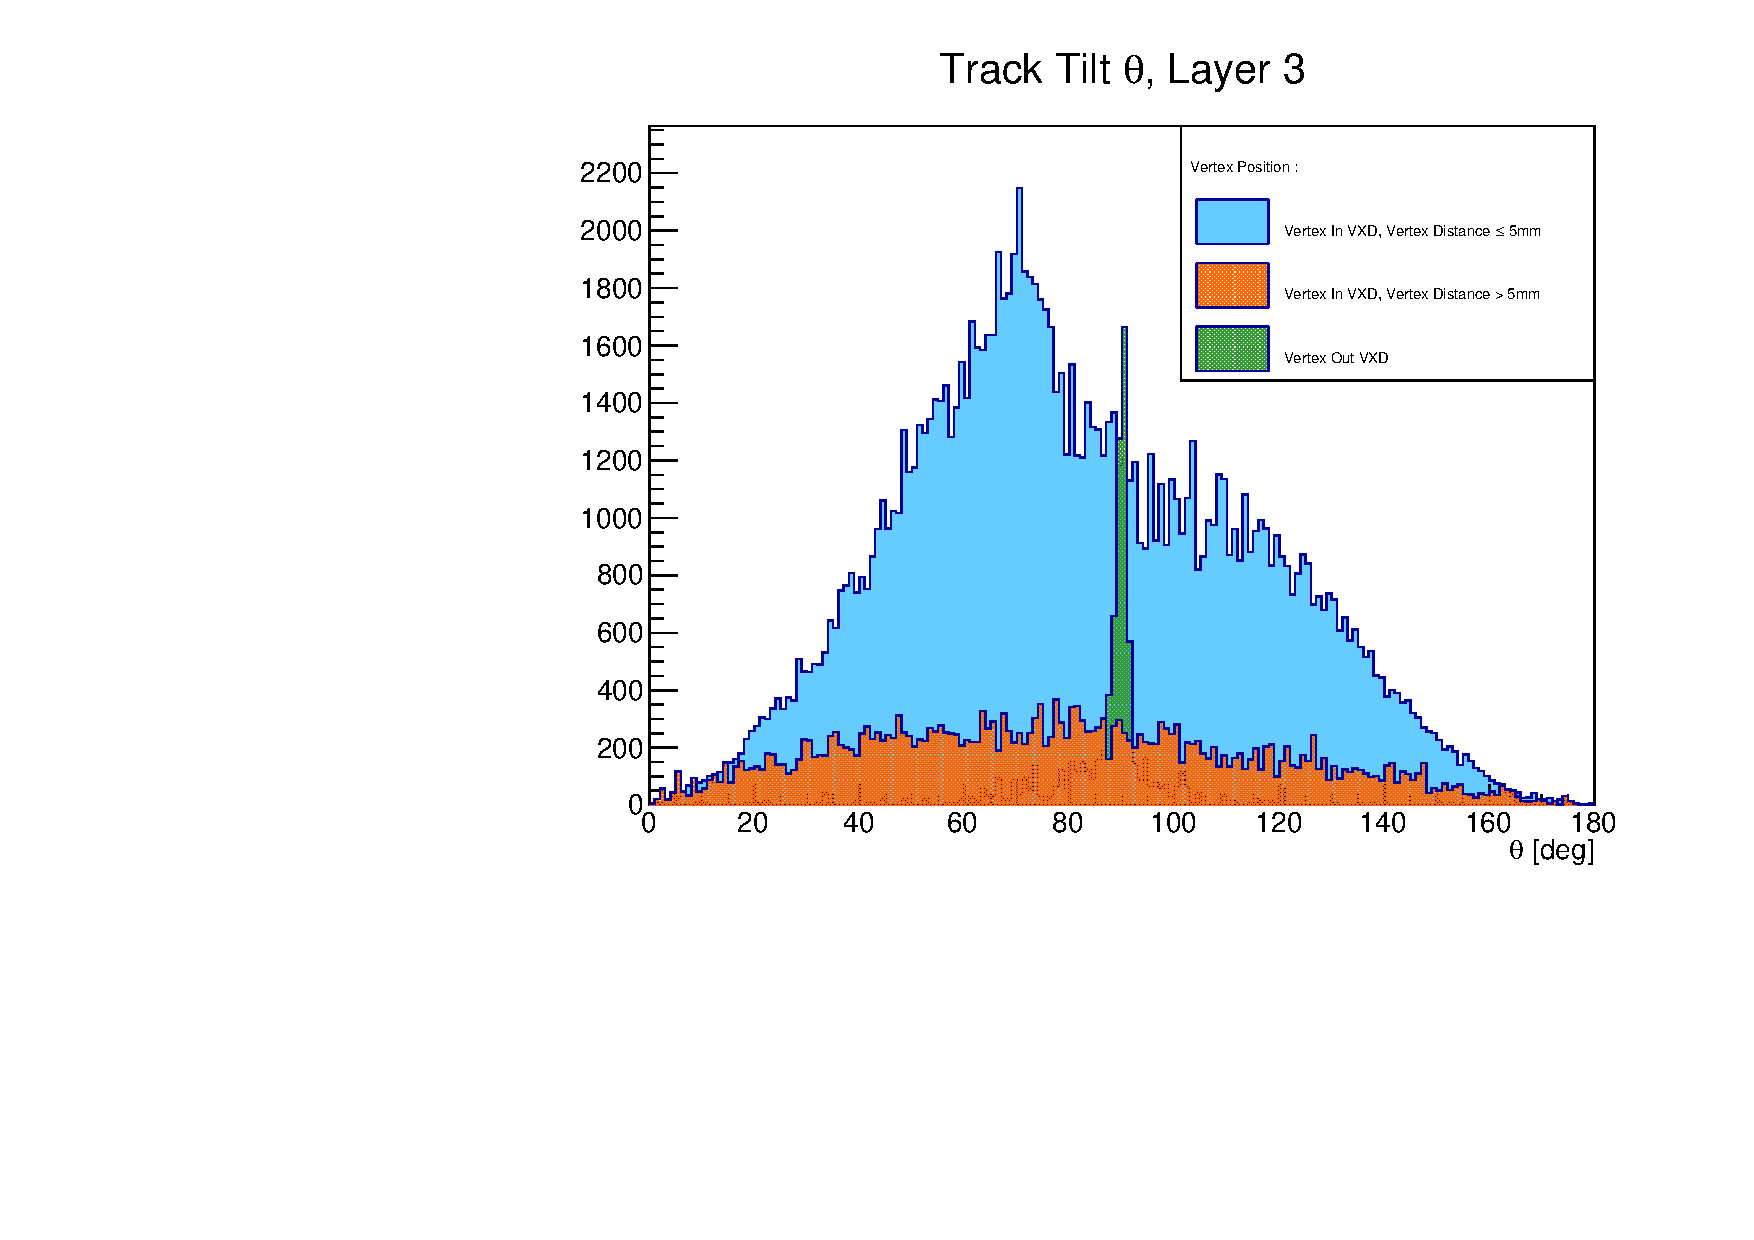
\includegraphics[scale=0.58]{./figures/Track_Tilts_Beamstrahlung/beamstrahlung_Theta/Track_Tilts_Theta_Layer3.pdf}
    \caption{Distribution des angles $\theta$ reconstruits pour chaque impact sur les \'echelles de la couche 3. Les couleurs bleue, rouge et verte distinguent les positions des vertex des particules associ\'ees aux impacts.}
    \label{fig:theta_Layer3}
  \end{figure}
  
  \begin{figure}[!htb]
    \centering    
    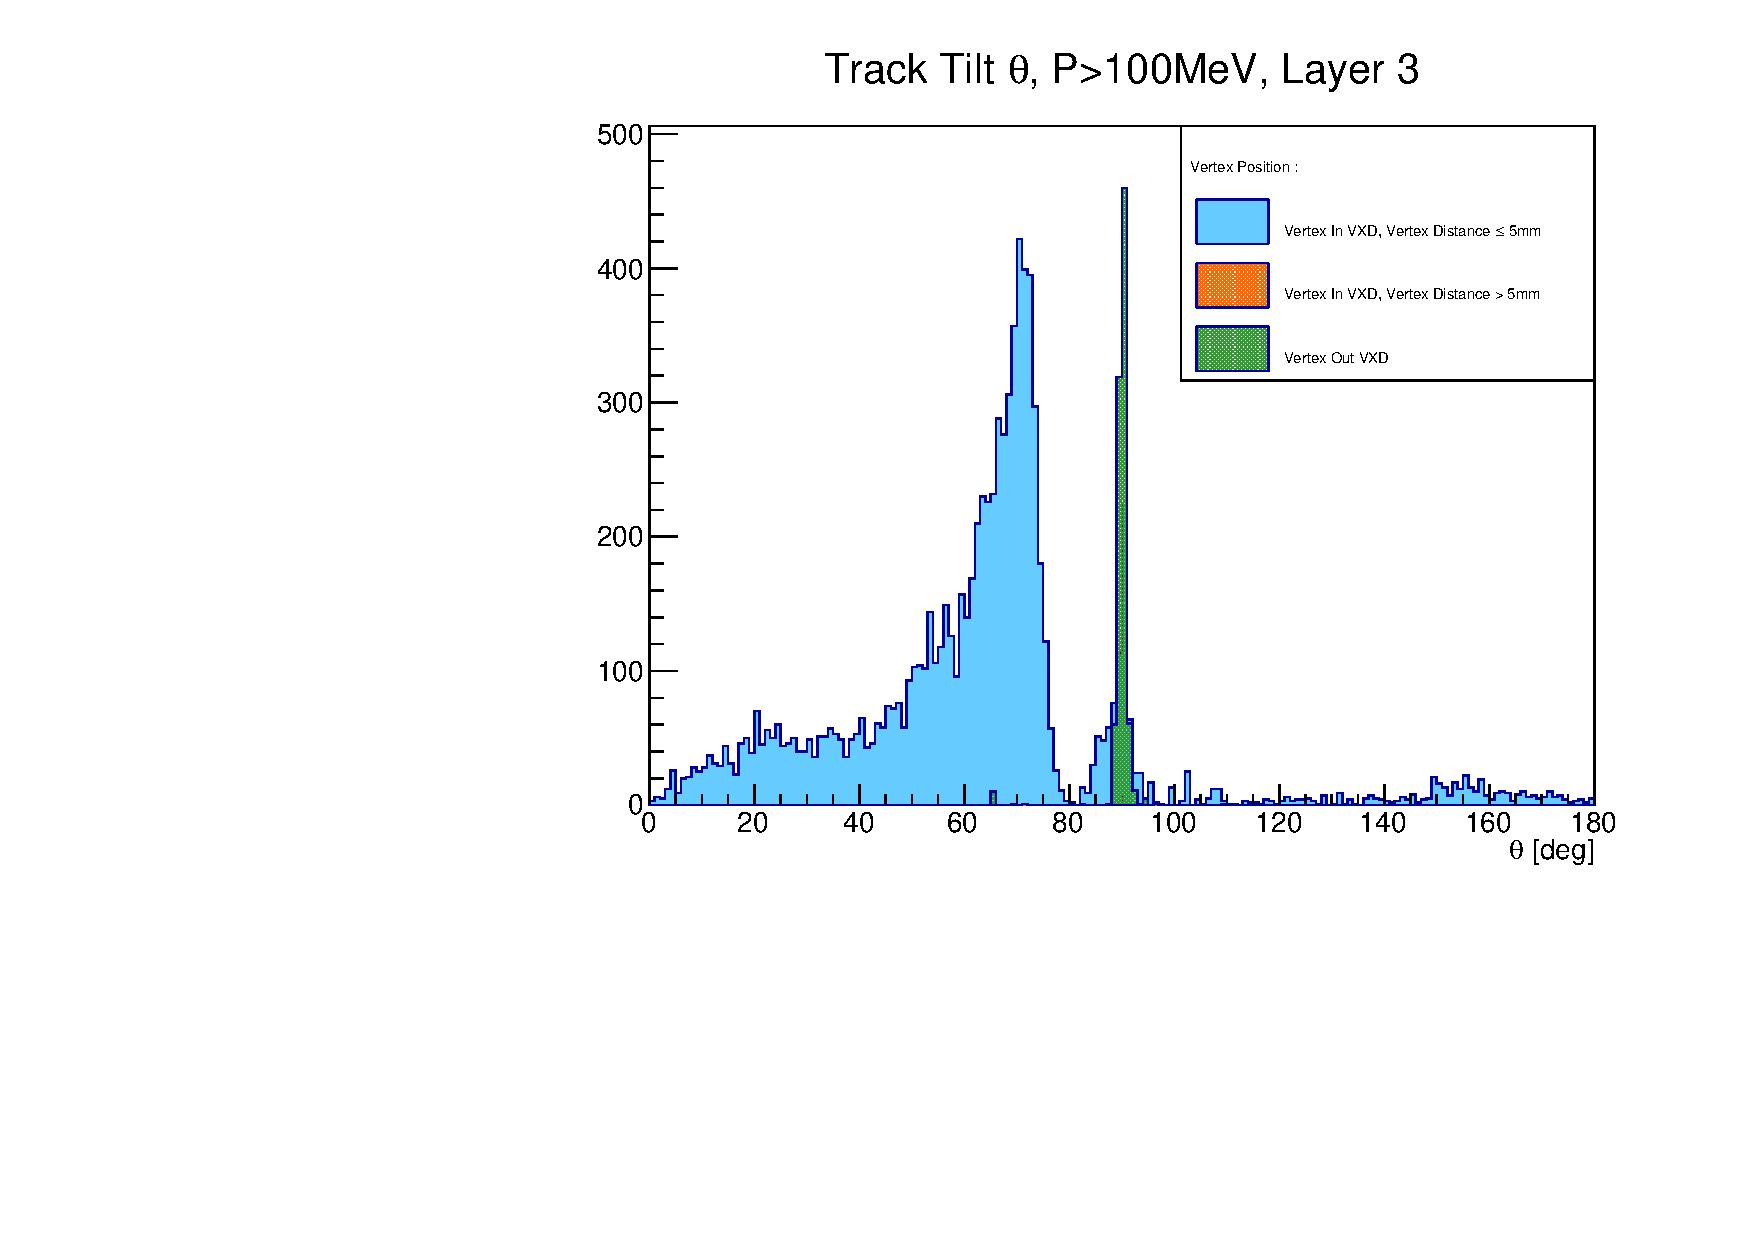
\includegraphics[scale=0.58]{./figures/Track_Tilts_Beamstrahlung/beamstrahlung_Theta/Track_Tilts_Theta_P_sup_100MeV_Layer3.pdf}
    \caption{Angle d'incidence $\theta$ associ\'e aux impacts de bruit de fond d'impulsion sup\'erieure \`a $100 MeV/c$ de la couche 3 en fonction de la position des impacts selon l'axe $U$ de l'\'echelle consid\'er\'ee.}
    \label{fig:theta_Layer3_pT_sup_100MeV}
  \end{figure}

  \begin{figure}[!htb]
    \centering
    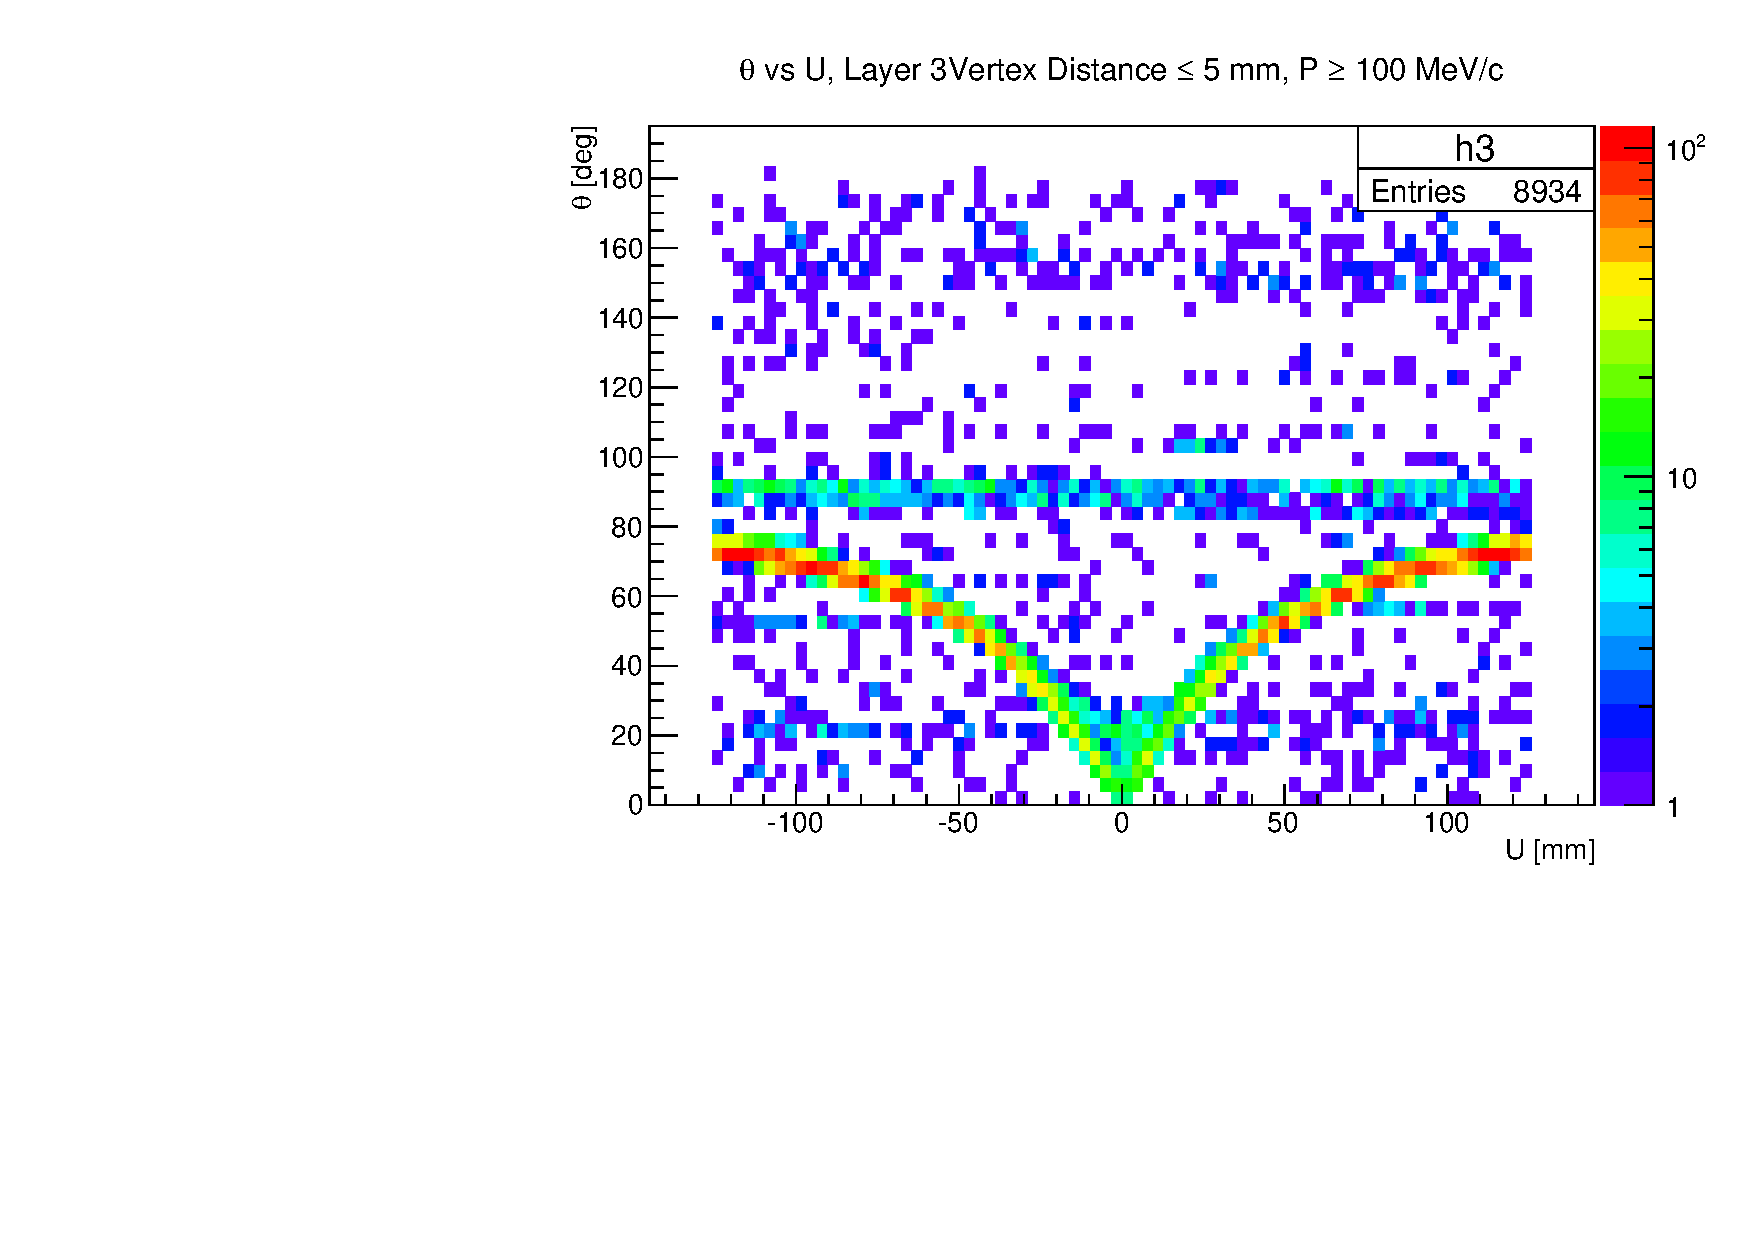
\includegraphics[scale=0.58]{./figures/Track_Tilts_Beamstrahlung/beamstrahlung_Theta/Track_Tilts_Theta_vs_U_P_sup_100MeV_vertex_inf_5mm_Layer3.pdf}
    \caption{Angle local $\phi$ associ\'e \`a chaque impact de bruit de fond de la couche 3 en fonction de la position de l'impact selon l'axe $U$ de l'\'echelle. Seuls les impacts dont le vertex de la particule correspondante est situ\'ee dans une sph\`ere de 5 $mm$ autour du point d'interaction sont trac\'es.}
    \label{fig:theta_Layer3_vs_U_P_sup_100MeV_vertex_inf_5mm}
  \end{figure}
 
  \begin{figure}[!htb]
    \centering
    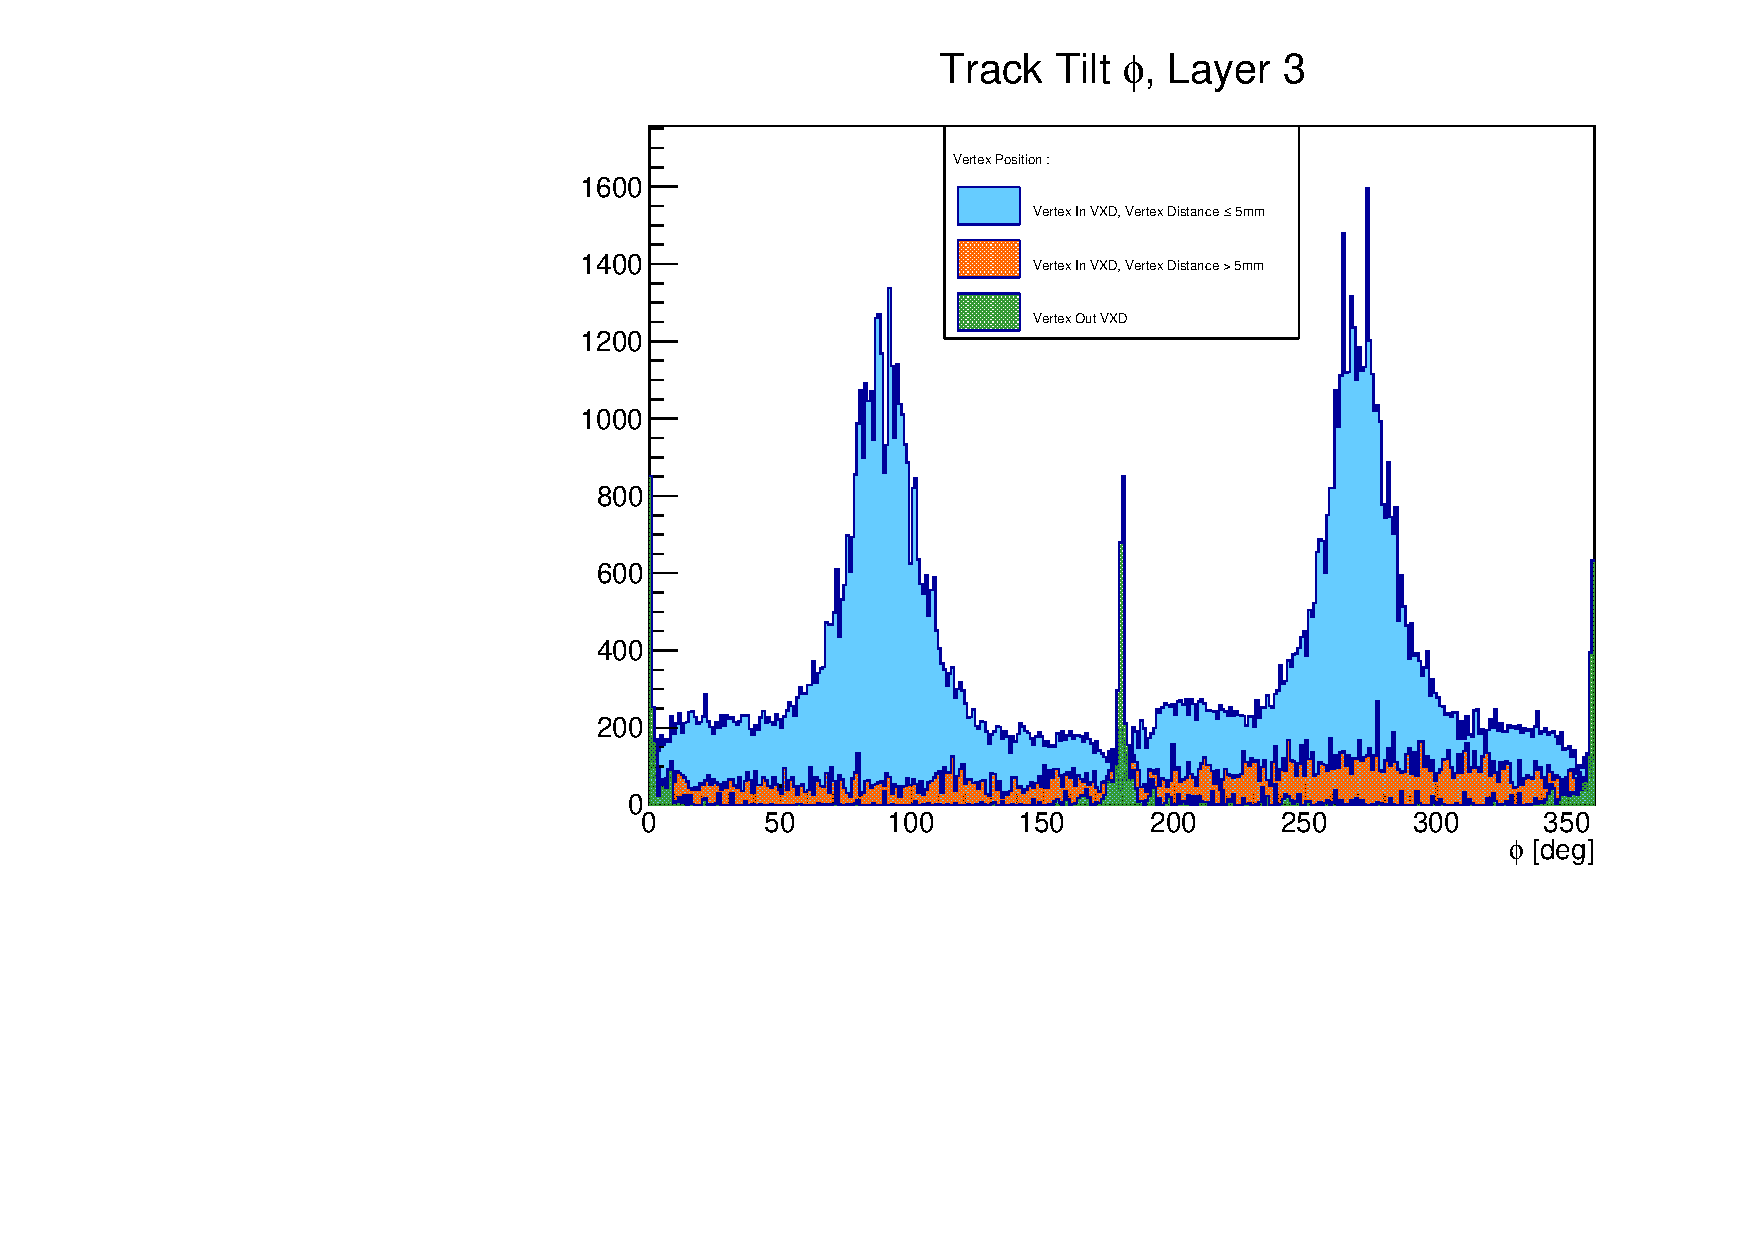
\includegraphics[scale=0.58]{./figures/Track_Tilts_Beamstrahlung/beamstrahlung_Phi/Track_Tilts_Phi_Layer3.pdf}
    \caption{Angle local $\phi$ associ\'e \`a chaque impact de bruit de fond de la couche 3.}
    \label{fig:phi_Layer3}
  \end{figure}
 
  \begin{figure}[!htb]
    \centering
    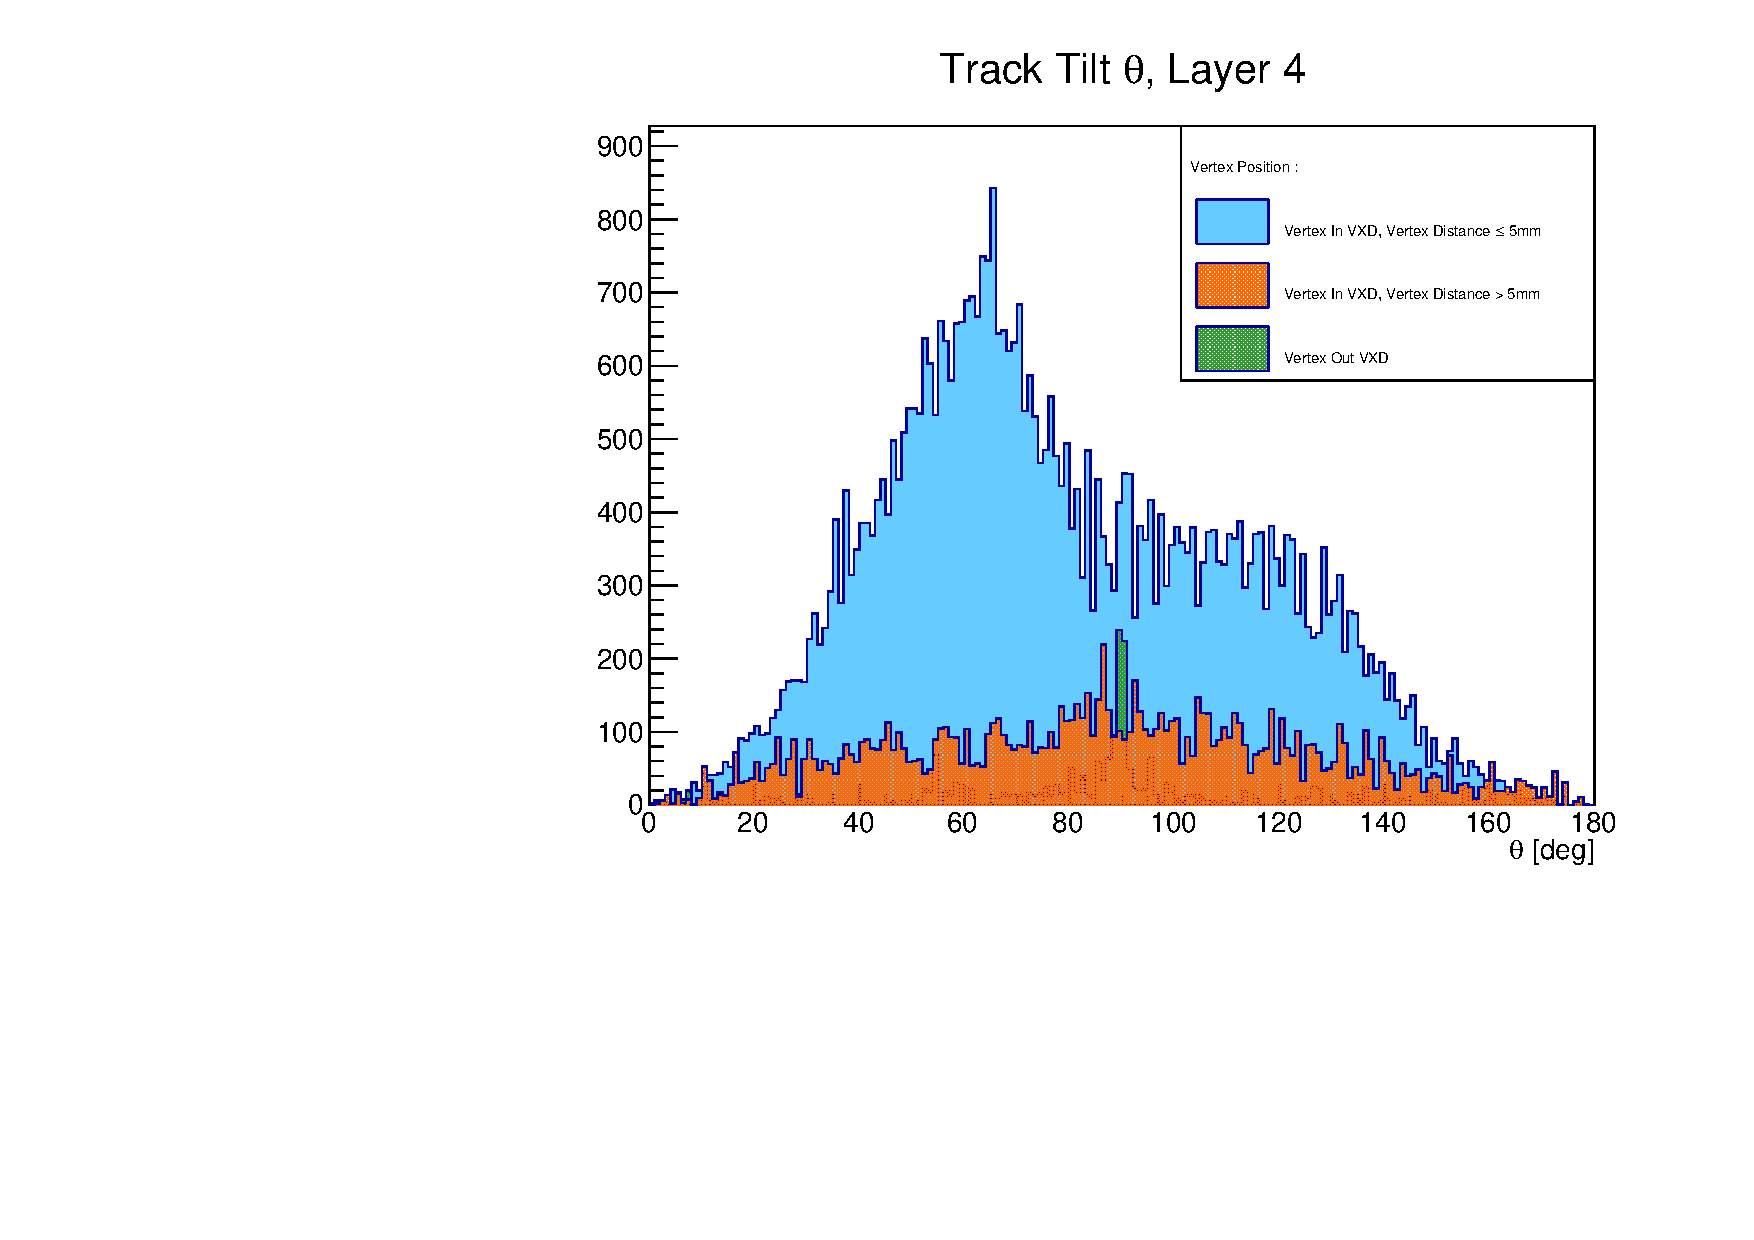
\includegraphics[scale=0.58]{./figures/Track_Tilts_Beamstrahlung/beamstrahlung_Theta/Track_Tilts_Theta_Layer4.pdf}
    \caption{Distribution des angles $\theta$ reconstruits pour chaque impact sur les \'echelles de la couche 4. Les couleurs bleue, rouge et verte distinguent les positions des vertex des particules associ\'ees aux impacts.}
    \label{fig:theta_Layer4}
  \end{figure}  
  
  \begin{figure}[!htb]
    \centering
    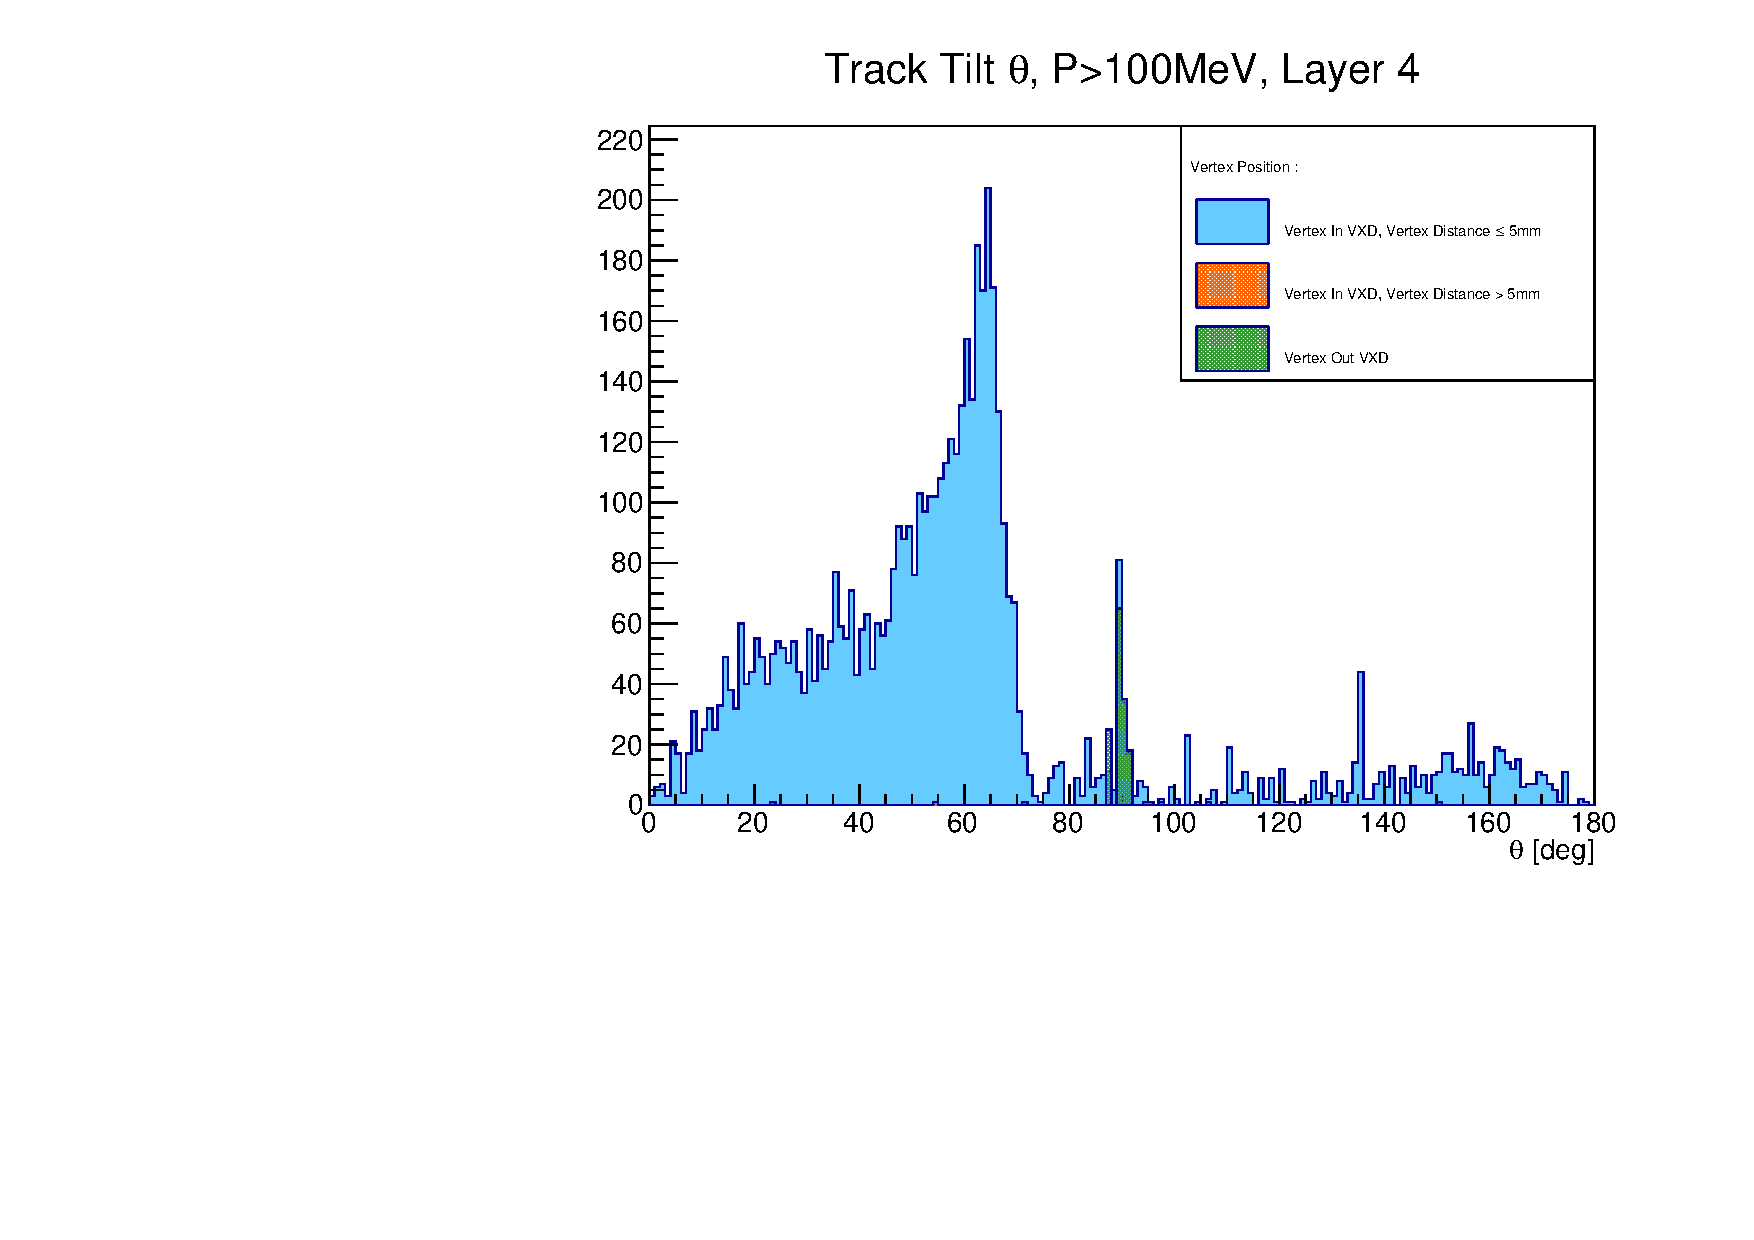
\includegraphics[scale=0.58]{./figures/Track_Tilts_Beamstrahlung/beamstrahlung_Theta/Track_Tilts_Theta_P_sup_100MeV_Layer4.pdf}
    \caption{Angle d'incidence $\theta$ associ\'e aux impacts de bruit de fond d'impulsion sup\'erieure \`a $100 MeV/c$ de la couche 4 en fonction de la position des impacts selon l'axe $U$ de l'\'echelle consid\'er\'ee.}
    \label{fig:theta_Layer4_pT_sup_100MeV}
  \end{figure}  

  \begin{figure}[!htb]
    \centering
    \includegraphics[scale=0.58]{./figures/Track_Tilts_Beamstrahlung/beamstrahlung_Theta/Track_Tilts_Theta_vs_U_P_sup_100MeV_vertex_inf_5mm_Layer4.pdf}
    \caption{Angle local $\phi$ associ\'e \`a chaque impact de bruit de fond de la couche 4 en fonction de la position de l'impact selon l'axe $U$ de l'\'echelle. Seuls les impacts dont le vertex de la particule correspondante est situ\'ee dans une sph\`ere de 5 $mm$ autour du point d'interaction sont trac\'es.}
    \label{fig:theta_Layer4_vs_U_P_sup_100MeV_vertex_inf_5mm}
  \end{figure}
  
  \begin{figure}
    \centering
    \includegraphics[scale=0.58]{./figures/Track_Tilts_Beamstrahlung/beamstrahlung_Phi/Track_Tilts_Phi_Layer4.pdf}
    \caption{Angle local $\phi$ associ\'e \`a chaque impact de bruit de fond de la couche 4.}
    \label{fig:phi_Layer4}
  \end{figure}
  
%    \clearpage
  
  \begin{figure}[!htb]
    \centering
    \includegraphics[scale=0.58]{./figures/Track_Tilts_Beamstrahlung/beamstrahlung_Theta/Track_Tilts_Theta_Layer5.pdf}
    \caption{Distribution des angles $\theta$ reconstruits pour chaque impact sur les \'echelles de la couche 5. Les couleurs bleue, rouge et verte distinguent les positions des vertex des particules associ\'ees aux impacts.}
    \label{fig:theta_Layer5}
  \end{figure}
  
  \begin{figure}[!phtb]
    \centering
    \includegraphics[scale=0.58]{./figures/Track_Tilts_Beamstrahlung/beamstrahlung_Theta/Track_Tilts_Theta_P_sup_100MeV_Layer5.pdf}
    \caption{Angle d'incidence $\theta$ associ\'e aux impacts de bruit de fond d'impulsion sup\'erieure \`a $100 MeV/c$ de la couche 5 en fonction de la position des impacts selon l'axe $U$ de l'\'echelle consid\'er\'ee.}
    \label{fig:theta_Layer5_pT_sup_100MeV}
  \end{figure}
  
  \begin{figure}[!htb]
    \centering
    \includegraphics[scale=0.58]{./figures/Track_Tilts_Beamstrahlung/beamstrahlung_Theta/Track_Tilts_Theta_vs_U_P_sup_100MeV_vertex_inf_5mm_Layer5.pdf}
    \caption{Angle local $\phi$ associ\'e \`a chaque impact de bruit de fond de la couche 5 en fonction de la position de l'impact selon l'axe $U$ de l'\'echelle. Seuls les impacts dont le vertex de la particule correspondante est situ\'ee dans une sph\`ere de 5 $mm$ autour du point d'interaction sont trac\'es.}
    \label{fig:theta_Layer5_vs_U_P_sup_100MeV_vertex_inf_5mm}
  \end{figure}
  
  \begin{figure}[!htb]
    \centering
    \includegraphics[scale=0.58]{./figures/Track_Tilts_Beamstrahlung/beamstrahlung_Phi/Track_Tilts_Phi_Layer5.pdf}
    \caption{Angle local $\phi$ associ\'e \`a chaque impact de bruit de fond de la couche 5.}
    \label{fig:phi_Layer5}
  \end{figure}

  \section{Taux d'occupation moyens des capteurs des couches 1 \`a 5 :}
  \label{annexe:tx_occ_moy}
  
     \begin{figure}[!htb]
    \begin{center}
      \includegraphics[scale=0.80]{./figures/sensors_Readout_Time/resultOccupancyPerSensor/occupancyPerSensor_Layer1_epi15um.pdf}
      \caption{Taux d'occupation moyens obtenus avec notre m\'ethode pour les capteurs la couche num\'ero 1 en fonction du temps de lecture de ceux-ci. Une couche \'epitaxi\'ee de 15 $\mu m$ et des pixels de $22 \times 33 \mu m^2$ sont utilis\'es.}
      \label{fig:OccupancyLayer1_epi15um}
    \end{center}
  \end{figure}

  \begin{figure}[!htb]
    \begin{center}
      \includegraphics[scale=0.80]{./figures/sensors_Readout_Time/resultOccupancyPerSensor/occupancyPerSensor_Layer1_epi30um.pdf}
      \caption{Taux d'occupation moyens obtenus avec notre m\'ethode pour les capteurs la couche num\'ero 1 en fonction du temps de lecture de ceux-ci. Une couche \'epitaxi\'ee de 30 $\mu m$ et des pixels de $22 \times 33 \mu m^2$ sont utilis\'es.}
      \label{fig:OccupancyLayer1_epi30um}
    \end{center}
  \end{figure}
  
   \begin{figure}[!htb]
    \begin{center}
      \includegraphics[scale=0.80]{./figures/sensors_Readout_Time/resultOccupancyPerSensor/occupancyPerSensor_Layer2_epi15um.pdf}
      \caption{Taux d'occupation moyens obtenus avec notre m\'ethode pour les capteurs la couche num\'ero 2 en fonction du temps de lecture de ceux-ci. Une couche \'epitaxi\'ee de 15 $\mu m$ et des pixels de $25 \times 50 \mu m^2$ ou $34 \times 34 \mu m^2$ sont utilis\'es.}
      \label{fig:OccupancyLayer2_epi15um}
    \end{center}
  \end{figure}

   \begin{figure}[!htb]
    \begin{center}
      \includegraphics[scale=0.80]{./figures/sensors_Readout_Time/resultOccupancyPerSensor/occupancyPerSensor_Layer2_epi30um.pdf}
      \caption{Taux d'occupation moyens obtenus avec notre m\'ethode pour les capteurs la couche num\'ero 2 en fonction du temps de lecture de ceux-ci. Une couche \'epitaxi\'ee de 30 $\mu m$ et des pixels de $25 \times 50 \mu m^2$ ou $34 \times 34 \mu m^2$ sont utilis\'es.}
      \label{fig:OccupancyLayer2_epi30um}
    \end{center}
  \end{figure}
  
   \begin{figure}[!htb]
    \begin{center}
      \includegraphics[scale=0.80]{./figures/sensors_Readout_Time/resultOccupancyPerSensor/occupancyPerSensor_Layer3_epi15um.pdf}
      \caption{Taux d'occupation moyens obtenus avec notre m\'ethode pour les capteurs la couche num\'ero 3 en fonction du temps de lecture de ceux-ci. Une couche \'epitaxi\'ee de 15 $\mu m$ et des pixels de $25 \times 50 \mu m^2$ ou $34 \times 34 \mu m^2$ sont utilis\'es.}
      \label{fig:OccupancyLayer3_epi15um}
    \end{center}
  \end{figure}

   \begin{figure}[!htb]
    \begin{center}
      \includegraphics[scale=0.80]{./figures/sensors_Readout_Time/resultOccupancyPerSensor/occupancyPerSensor_Layer3_epi30um.pdf}
      \caption{Taux d'occupation moyens obtenus avec notre m\'ethode pour les capteurs la couche num\'ero 3 en fonction du temps de lecture de ceux-ci. Une couche \'epitaxi\'ee de 30 $\mu m$ et des pixels de $25 \times 50 \mu m^2$ ou $34 \times 34 \mu m^2$ sont utilis\'es.}
      \label{fig:OccupancyLayer3_epi30um}
    \end{center}
  \end{figure}
  
   \begin{figure}[!htb]
    \begin{center}
      \includegraphics[scale=0.80]{./figures/sensors_Readout_Time/resultOccupancyPerSensor/occupancyPerSensor_Layer4_epi15um.pdf}
      \caption{Taux d'occupation moyens obtenus avec notre m\'ethode pour les capteurs la couche num\'ero 4 en fonction du temps de lecture de ceux-ci. Une couche \'epitaxi\'ee de 15 $\mu m$ et des pixels de $25 \times 50 \mu m^2$ ou $34 \times 34 \mu m^2$ sont utilis\'es.}
      \label{fig:OccupancyLayer4_epi15um}
    \end{center}
  \end{figure}

   \begin{figure}[!htb]
    \begin{center}
      \includegraphics[scale=0.80]{./figures/sensors_Readout_Time/resultOccupancyPerSensor/occupancyPerSensor_Layer4_epi30um.pdf}
      \caption{Taux d'occupation moyens obtenus avec notre m\'ethode pour les capteurs la couche num\'ero 4 en fonction du temps de lecture de ceux-ci. Une couche \'epitaxi\'ee de 30 $\mu m$ et des pixels de $25 \times 50 \mu m^2$ ou $34 \times 34 \mu m^2$ sont utilis\'es.}
      \label{fig:OccupancyLayer4_epi30um}
    \end{center}
  \end{figure}  

   \begin{figure}[!htb]
    \begin{center}
      \includegraphics[scale=0.80]{./figures/sensors_Readout_Time/resultOccupancyPerSensor/occupancyPerSensor_Layer5_epi15um.pdf}
      \caption{Taux d'occupation moyens obtenus avec notre m\'ethode pour les capteurs la couche num\'ero 5 en fonction du temps de lecture de ceux-ci. Une couche \'epitaxi\'ee de 15 $\mu m$ et des pixels de $25 \times 50 \mu m^2$ ou $34 \times 34 \mu m^2$ sont utilis\'es.}
      \label{fig:OccupancyLayer5_epi15um}
    \end{center}
  \end{figure}

   \begin{figure}[!htb]
    \begin{center}
      \includegraphics[scale=0.80]{./figures/sensors_Readout_Time/resultOccupancyPerSensor/occupancyPerSensor_Layer5_epi30um.pdf}
      \caption{Taux d'occupation moyens obtenus avec notre m\'ethode pour les capteurs la couche num\'ero 5 en fonction du temps de lecture de ceux-ci. Une couche \'epitaxi\'ee de 30 $\mu m$ et des pixels de $25 \times 50 \mu m^2$ ou $34 \times 34 \mu m^2$ sont utilis\'es.}
      \label{fig:OccupancyLayer5_epi30um}
    \end{center}
  \end{figure}
  
  
  \section{Taux d'occupation minimums et maximums pour les couche 1 \`a 5 :}
  \label{annexe:Tx_Occ_Min_Max}
    
  \begin{figure}[!htb]
    \begin{center}
      \includegraphics[scale=0.80]{./figures/sensors_Readout_Time/resultOccupancyPerSensor/occupancyPerSensor_Layer1_epi_15um_Min_Max.pdf}
      \caption{Taux d'occupation moyens, minimums et maximums obtenus avec notre m\'ethode pour les capteurs la couche num\'ero 1. Une couche \'epitaxi\'ee de 15 $\mu m$, des pixels de $22 \times 33 \mu m^2$ et un temps de lecture de 4 $\mu s$ sont utilis\'es.}
      \label{fig:OccupancyLayer1_epi15um_Min_Max}
    \end{center}
  \end{figure}
  
  \begin{figure}[!htb]
    \begin{center}
      \includegraphics[scale=0.80]{./figures/sensors_Readout_Time/resultOccupancyPerSensor/occupancyPerSensor_Layer1_epi_30um_Min_Max.pdf}
      \caption{Taux d'occupation moyens, minimums et maximums obtenus avec notre m\'ethode pour les capteurs la couche num\'ero 1. Une couche \'epitaxi\'ee de 30 $\mu m$, des pixels de $22 \times 33 \mu m^2$ et un temps de lecture de 4 $\mu s$ sont utilis\'es.}
      \label{fig:OccupancyLayer1_epi30um_Min_Max}
    \end{center}
  \end{figure}
  
  \begin{figure}[!htb]
    \begin{center}
      \includegraphics[scale=0.80]{./figures/sensors_Readout_Time/resultOccupancyPerSensor/occupancyPerSensor_Layer2_epi_15um_Min_Max.pdf}
      \caption{Taux d'occupation moyens, minimums et maximums obtenus avec notre m\'ethode pour les capteurs la couche num\'ero 2. Une couche \'epitaxi\'ee de 15 $\mu m$, des pixels de $25 \times 50 \mu m^2$ et un temps de lecture de 80 $\mu s$ sont utilis\'es.}
      \label{fig:OccupancyLayer2_epi15um_Min_Max}
    \end{center}
  \end{figure}
  
  \begin{figure}[!htb]
    \begin{center}
      \includegraphics[scale=0.80]{./figures/sensors_Readout_Time/resultOccupancyPerSensor/occupancyPerSensor_Layer2_epi_30um_Min_Max.pdf}
      \caption{Taux d'occupation moyens, minimums et maximums obtenus avec notre m\'ethode pour les capteurs la couche num\'ero 2. Une couche \'epitaxi\'ee de 30 $\mu m$, des pixels de $25 \times 50 \mu m^2$ et un temps de lecture de 80 $\mu s$ sont utilis\'es.}
      \label{fig:OccupancyLayer2_epi30um_Min_Max}
    \end{center}
  \end{figure}
  
  \begin{figure}[!htb]
    \begin{center}
      \includegraphics[scale=0.80]{./figures/sensors_Readout_Time/resultOccupancyPerSensor/occupancyPerSensor_Layer3_epi_15um_Min_Max.pdf}
      \caption{Taux d'occupation moyens, minimums et maximums obtenus avec notre m\'ethode pour les capteurs la couche num\'ero 3. Une couche \'epitaxi\'ee de 15 $\mu m$, des pixels de $25 \times 50 \mu m^2$ et un temps de lecture de 80 $\mu s$ sont utilis\'es.}
      \label{fig:OccupancyLayer3_epi15um_Min_Max}
    \end{center}
  \end{figure}

  \begin{figure}[!htb]
    \begin{center}
      \includegraphics[scale=0.80]{./figures/sensors_Readout_Time/resultOccupancyPerSensor/occupancyPerSensor_Layer3_epi_30um_Min_Max.pdf}
      \caption{Taux d'occupation moyens, minimums et maximums obtenus avec notre m\'ethode pour les capteurs la couche num\'ero 3. Une couche \'epitaxi\'ee de 30 $\mu m$, des pixels de $25 \times 50 \mu m^2$ et un temps de lecture de 80 $\mu s$ sont utilis\'es.}
      \label{fig:OccupancyLayer3_epi30um_Min_Max}
    \end{center}
  \end{figure}
  
  \begin{figure}[!htb]
    \begin{center}
      \includegraphics[scale=0.80]{./figures/sensors_Readout_Time/resultOccupancyPerSensor/occupancyPerSensor_Layer4_epi_15um_Min_Max.pdf}
      \caption{Taux d'occupation moyens, minimums et maximums obtenus avec notre m\'ethode pour les capteurs la couche num\'ero 4. Une couche \'epitaxi\'ee de 15 $\mu m$, des pixels de $25 \times 50 \mu m^2$ et un temps de lecture de 80 $\mu s$ sont utilis\'es.}
      \label{fig:OccupancyLayer4_epi15um_Min_Max}
    \end{center}
  \end{figure}
  
  \begin{figure}[!htb]
    \begin{center}
      \includegraphics[scale=0.80]{./figures/sensors_Readout_Time/resultOccupancyPerSensor/occupancyPerSensor_Layer4_epi_30um_Min_Max.pdf}
      \caption{Taux d'occupation moyens, minimums et maximums obtenus avec notre m\'ethode pour les capteurs la couche num\'ero 4. Une couche \'epitaxi\'ee de 30 $\mu m$, des pixels de $25 \times 50 \mu m^2$ et un temps de lecture de 80 $\mu s$ sont utilis\'es.}
      \label{fig:OccupancyLayer4_epi30um_Min_Max}
    \end{center}
  \end{figure}

  \begin{figure}[!htb]
    \begin{center}
      \includegraphics[scale=0.80]{./figures/sensors_Readout_Time/resultOccupancyPerSensor/occupancyPerSensor_Layer5_epi_15um_Min_Max.pdf}
      \caption{Taux d'occupation moyens, minimums et maximums obtenus avec notre m\'ethode pour les capteurs la couche num\'ero 5. Une couche \'epitaxi\'ee de 15 $\mu m$, des pixels de $25 \times 50 \mu m^2$ et un temps de lecture de 80 $\mu s$ sont utilis\'es.}
      \label{fig:OccupancyLayer5_epi15um_Min_Max}
    \end{center}
  \end{figure}
  
  \begin{figure}[!htb]
    \begin{center}
      \includegraphics[scale=0.80]{./figures/sensors_Readout_Time/resultOccupancyPerSensor/occupancyPerSensor_Layer5_epi_30um_Min_Max.pdf}
      \caption{Taux d'occupation moyens, minimums et maximums obtenus avec notre m\'ethode pour les capteurs la couche num\'ero 5. Une couche \'epitaxi\'ee de 30 $\mu m$, des pixels de $25 \times 50 \mu m^2$ et un temps de lecture de 80 $\mu s$ sont utilis\'es.}
      \label{fig:OccupancyLayer5_epi30um_Min_Max}
    \end{center}
  \end{figure}  
  
  
  
\end{appendices} 